\documentclass[12pt,a4paper]{article}
\usepackage[utf8x]{inputenc}
\usepackage[czech]{babel}
\usepackage[T1]{fontenc}
\setlength{\parskip}{12pt}
\usepackage{fullpage}
\setlength{\parskip}{6pt}
\usepackage{ amssymb }
\usepackage{ mathrsfs }
\usepackage{amsthm}
\usepackage{amsmath}
\usepackage{fixltx2e}
\newtheorem{definition}{Definice}
\newtheorem{sentence}{Věta}
\newtheorem{example}{Příklad}
\newtheorem{result}{Důsledek}
\usepackage{graphicx}
\usepackage{ dsfont }
\usepackage{color}
\usepackage{float}

\begin{document}

\title{Státnicový okruh 1: \\ Matematické metody}
\maketitle
\newpage
\tableofcontents
\newpage
% ---------------------------------------------------------------------------------------------------------
% --------------------------------------------- první odstavec ---------------------------------------------
% ---------------------------------------------------------------------------------------------------------
\textbf{Množiny, operace s množinami, kartézský součin množin, konečné, spočetné a nespočetné množiny. Číselné
množiny. Princip indukce. Relace a jejich vlastnosti, operace s relacemi, reprezentace relací. Binární relace na
množině, uzávěry relací, ekvivalence, rozklad na množině, uspořádané množiny. Zobrazení a jejich vlastnosti.}

\section{Množiny}
Množina je objekt, který se skládá z jiných objektů tzv. \textbf{prvků} té množiny. Množiny zpravidla značíme velkými písmeny (A, B, \dots, Z), jejich prvky pak malými písmeny (a, b, \dots, z). Fakt, že $x$ je prvkem množiny $A$ značíme $x \in A$. Není-li prvkem $A$ značíme $x \not\in A$.

Množina je jednoznačné dána svými prvky. Prvek do množiny buď patní nebo ne. Nemá tedy smysl hovořit o pořadí prvků a také nemá smysl zabývat se tím kolikrát se daný prvek v množině nachází.
Speciální množinou je tzv. \textbf{prázdná množina} značíme $\emptyset$. Tato množina neobsahuje žádné prvky tedy pro všechna $x$ platí, že $x \not\in \emptyset$.

\subsection{Dělení množin}
Množiny dělíme na \textbf{konečné} a \textbf{nekonečné}. Množina $A$ se nazývá konečná právě když existuje přirozené číslo $n$ tak že prvky této množiny můžeme očíslovat čísly 1, 2, \dots, $n$. Číslo $n$ nazveme počet prvků množiny a značíme jej $|A|$
Pokud $|A| = \infty$ nazveme množinu nekonečnou a říkáme, že má nekonečně mnoho prvků.

\textbf{Spočetná} množina znamená zjednodušeně řečeno „množina, jejíž prvky lze spočítat“. Spočítáním se zde rozumí očíslování prvků množiny přirozenými čísly - přitom je jedno, zda použiji konečný nebo nekonečný počet přirozených čísel.

\subsection{Zapisování množin}
Množiny můžeme zapisovat následujícími způsoby:
\begin{enumerate}
	\item \textbf{Výčtem prvků} - Množinu která obsahuje prvky $a_1,a_2,\dots,a_n$ zapíšeme následovně $\{a_1,a_2,\dots,a_n\}$.
	\item \textbf{Pomocí charakteristické vlastnosti} - Množina obsahuje právě ty prvky, které splňují vlastnost $\varphi(x)$ zapisujeme $\{x | \varphi(x)\}$. Vlastnost $\varphi(x)$ může být popsána i slovně. Příklad $\varphi(x)$: číslo x je sudé.
\end{enumerate}
\subsection{Vztahy mezi množinami}
Základními vztahy mezi množinami jsou \textbf{rovnost} (=) a \textbf{inkluze} ($\subseteq$)
\begin{itemize}
	\item[] $A = B$ znamená, že pro každé $x : x \in A$ právě když $x \in B$
	\item[] $A \subseteq B$ znamená, že pro každé $x$ : jestliže $x \in A$ pak $x \in B$
	\item[] $A \not= B$ znamená že neplatí $A = B$
	\item[] $A \not\subseteq B$ znamená, že neplatí $A \subseteq B$
\end{itemize}

Množina jejichž prvky jsou právě všechny podmnožiny dané množiny $X$, nazýváme \textbf{potenční množina} množiny $X$ značí se $\mathscr{P}(X)$ nebo také $2^X$. Tedy $2^X = \{A|A\subseteq X\}$.

\subsection{Operace s množinami}
Mezi základní operace s množinami patří průnik (značí se $\cap$), sjednocení (značí se $\cup$), rozdíl (značí se $\setminus$).

Jsou-li $A,B$ množiny, definujeme množiny $A \cup B, A \cap B, A \setminus B$ následovně:
\begin{itemize}
	\item[] $A \cap B = \{ x|x \in A \text{ a } x \in B\}$
	\item[] $A \cup B = \{ x|x \in A \text{ nebo } x \in B\}$
	\item[] $A \setminus B = \{ x|x \in A \text{ a } x \not\in B\}$
\end{itemize}

Množiny nazýváme navzájem disjunktní právě když $A \cap B = \emptyset$.

\subsubsection{Vlastnosti operací}
\begin{itemize}
	\item $A \cap \emptyset = \emptyset, \hspace{10pt} A \cup \emptyset = A,\hspace{10pt} A \cap A = A$
	\item $A \cup B = B \cup A, \hspace{10pt} A \cap B = B \cap A$
	\item $(A \cup B) \cup C = A \cup (B \cup C)$
	\item $A \cap (B \cup C) = (A \cap B) \cup (A \cap C), \hspace{10pt} A \cup (B \cap C) = (A \cup B) \cap (A \cup C)$
	\item $A \cup (A \cap B) = A, \hspace{10pt} A \cap (A \cup B) = A$
\end{itemize}

\section{Princip indukce}
Princip matematické indukce umožňuje dokazovat tvrzení ve tvaru \uv{pro každé přirozené číslo $n$ platí $V(n)$}, kde $V(n)$ je nějaké tvrzení, které závisí na $n$ (např. $1 + 2 + \dots + n = \frac{n(n+1)}{2}$).

\begin{sentence}
	Nechť je pro každé $n \in \mathbb{N}$ dáno tvrzení $V(n)$. Předpokládejme že platí
	\begin{itemize}
		\item V(1) (indukční předpoklad)
		\item pro každé $n \in \mathbb{N}$: z V(n) plyne V($n+1$) (indukční krok).
	\end{itemize}
	Pak platí V(n) pro každé $n \in \mathbb{N}$.
\end{sentence}

Princip indukce je jednou ze základních vlastností přirozených čísel, Z předpokladu, že každá neprázdná podmnožina $K \subseteq \mathbb{N}$má nejmenší prvek (což je pravdivý a intuitivně jasný předpoklad) lze princip indukce dokázat.

\begin{example}
	Dokažte už uvedený vztah $1 + 2 + \dots + n = \frac{n(n+1)}{2}$. Tedy V(n) je tvrzení $\sum^n_{k=1} k =  \frac{n(n+1)}{2}$. Podle principu indukce stačí ověřit indukční předpoklad a indukční krok. \\[6pt]
	Indukční předpoklad: V(1) je tvrzení $1 = \frac{1 \cdot (1 + 1)}{2}$ a to evidentně platí.\\[6pt]
	Indukční krok: Předpokládejme, že platí V(n) a dokažme V($n + 1$). $1 + \dots + n + n + 1$ se rovná  $(1 + \dots + n) + n + 1$, což se dle předpokladu rovná $\frac{n(n + 1)}{2} + n + 1$. Dále je $\frac{n(n + 1)}{2} + n + 1 = \frac{n(n + 1) + 2(n + 1)}{2} = \frac{n^2 + 3n + 2}{2} = \frac{(n + 1) \cdot (n + 2)}{2}$. Celkem tedy $1 + \dots + n + n + 1 =  \frac{(n + 1) \cdot (n + 2)}{2}$, což je právě tvrzení V(n + 1).\\[6pt]
	Podle principu indukce je tedy tvrzení dokázané.
\end{example}

\section{Relace}
Pojem relace je matematickým protějškem pojmu \textit{vztah}. Různé objekty jsou nebo nejsou v různých vztazích. Například číslo 3 je ve vztahu \uv{být menší} s číslem 5. Vztah je také určen aritou tj. počtem objektů které do vztahu vstupují, výše uvedený příklad má aritu 2 protože porovnáváme 2 čísla. Takovou relaci nazveme binární. Dále máme unární (jeden prvek), ternární (tři prvky), \dots

\begin{definition}
Kartézský součin množin $X_1, X_2, \dots,X_n$ je množina $X_1 \times X_2 \times \dots \times X_n$ definovaná předpisem $$X_1 \times \dots \times X_n =  \{\langle x_1, \dots x_n \rangle | x_1 \in X_1, \dots, x_n \in X_n\} $$
\end{definition}
 Kartézský součin $n$ množin je množina všech uspořádaných n-tic prvků z těchto množin. Je-li $X_1 = \dots = X_n = X$ pak $X_1 \times \dots \times X_n$ značíme také $X^n$ (n-tá kartézská mocnina množiny $X$)

\begin{definition}
Nechť $X_1, \dots,X_n$ jsou množiny. Relace mezi $X_1, \dots,X_n$ je libovolná podmnožina kartézského součinu $X_1 \times \dots \times X_n $.
\end{definition}

\begin{example}
Mějme množinu $A = \{1,2,3,4\}$ a množinu $B = \{a,b,c,d\}$. Relace $R,S \subseteq A \times B$ mohou vypadat následovně. $$R = \{\langle 1, a\rangle, \langle 1, b\rangle, \langle 3, d\rangle, \langle 4, a\rangle\}$$
$$S = \{\langle 3, a\rangle, \langle 1, c\rangle,  \langle 4, c\rangle\}\}$$
\end{example}

\subsection{Operace s (binárními) relacemi}
Relace jsou množiny n-tic. Proto s nimi jde provádět množinové operace ($\cap,\cup,\setminus$) a lze na ně aplikovat rovnost a inkluzi ($=, \subseteq$).
S binárními relacemi můžeme provádět další operace. Začněme tzv. inverzní relací k relaci $R \subseteq X \times Y$ je relace $R^{-1}$ definovaná předpisem: $$R^{-1} = \{\langle y, x \rangle | \langle x, y \rangle \in R\}$$
Další operací je tzv. skládání Je-li $R$ relací mezi množinami $X$ a $Y$ a $S$ relací mezi množinami $Y$ a $Z$, pak složením relací $R$ a $S$ je relace \( R \circ S \) mezi $X$ a $Z$ definovaná předpisem: $$R \circ S = \{\langle x, z \rangle | \exists y \in Y : \langle x,y\rangle \in R \text{ a } \langle y,z \rangle \in S\}$$

\begin{sentence}
	Pro relace $R \subseteq X \times Y, S \subseteq Y \times Z, T \subseteq Z \times U$ platí:
	\begin{itemize}
		\item[a)] $(R^{-1})^{-1} = R$
		\item[b)] $(R \circ S)^{-1} = S^{-1} \circ R^{-1}$
		\item[c)] $R \circ (S \circ T) = (R \circ S) \circ T$
	\end{itemize}
\end{sentence}

\subsection{Reprezentace relací}

\subsubsection{Tabulkou}
Binární relace lze znázorňovat tabulkami. Například relace \\$R = \{ \langle 1, \alpha \rangle, \langle 2, \gamma \rangle, \langle 1, \delta \rangle, \langle 2, \beta \rangle, \langle 3, \alpha \rangle\}$ mezi množinami \\$X = \{1,2,3\}$ a $Y = \{\alpha, \beta, \gamma, \delta, \epsilon\}$ je znázorněna následující tabulkou.

\begin{center}
	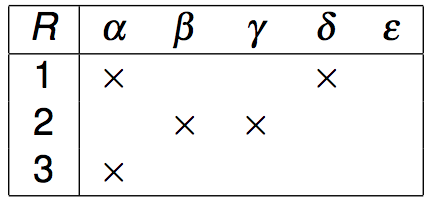
\includegraphics[scale=0.5]{img/RelationTable}
\end{center}

Tedy je-li $\langle x, y \rangle \in R$, je v průsečíku řádku $x$ a sloupce $y$ symbol $\times$, jinak tam není nic.

\subsubsection{Maticí}
Matice typu $m \times n$ je obdélníkové schéma o $m$ řádcích a $n$ sloupcích, ve kterém se na každém místě odpovídajícím nějakému řádku a nějakému sloupci nachází nějaká (nejčastěji číselná) hodnota. Označme tuto matici $M$, pro každé $i \in \{1, \dots,m\}$ a $j \in \{1,\dots,n\}$  Nechť $R$ je relace mezi množinami $X = \{x_1,\dots,x_m\}$ a $Y = \{y_1, \dots, y_n\}$. Potom relaci $R$ reprezentujeme maticí tak, že pokud:
$$\langle x_i,y_j\rangle \in R \text{ pak } m_{ij} = 1$$
$$\langle x_i,y_j\rangle \not\in R \text{ pak } m_{ij} = 0$$
Tuto matici nazveme \textbf{matice relace} R a značíme ji $M_R$. Matice $M_R$ relace $R = \{ \langle 1, \alpha \rangle, \langle 2, \gamma \rangle, \langle 1, \delta \rangle, \langle 2, \beta \rangle, \langle 3, \alpha \rangle\}$ mezi množinami \\$X = \{1,2,3\}$ a $Y = \{\alpha, \beta, \gamma, \delta, \epsilon\}$ bude vypadat  následovně.

\begin{displaymath}
{\bf M_R} =
\left( \begin{array}{ccccc}
1 & 0 & 0 & 1 & 0 \\
0 & 1 & 1 & 0 & 0 \\
1 & 0 & 0 & 0 & 0 \\
\end{array} \right)
\end{displaymath}

Nevýhodou této metody je její paměťová složitost. Pokud budeme mít matici $1000 \times 1000$, tak musíme v paměti uchovat milión prvků a pokud z nich bude jen 3000 rovno 1 potom zbytek uchováváme zbytečně protože víme, že na ostatních pozicích musí být 0.

Pro binární relace můžeme zavést operace, které odpovídají operacím s relacemi. Mějme binární matice $M,N$ typu $m \times n$ a matici $K$ typu $n \times k$. Definujeme následující operace:
\begin{itemize}
	\item[] $M \vee N = P, \qquad p_{ij} = max\{m_{ij}, n_{ij}\};$
	\item[] $M \wedge N = P, \qquad min\{m_{ij}, n_{ij}\};$
	\item[] $M - N = P, \qquad max\{0, m_{ij} - n_{ij}\};$
	\item[] $M \cdot K = P, \qquad max\{m_{ij} \cdot k_{ij}; I = 1, \dots ,n\};$
	\item[] $M^T, \qquad m^T_{ij} = m_{ji}$
\end{itemize}

\subsubsection{Grafem}
Grafy představují další způsob reprezentace binárních relací, který je názorný. Graf binární relace $R$ na množině $X$ dostaneme tak, že každý prvek $x \in X$ znázorníme v rovině jako kroužek s označením daného prvku. Pokud $\langle x,y \rangle \in R$, nakreslíme z uzlu $x$ do uzlu $y$ orientovanou hranu.

\begin{center}
	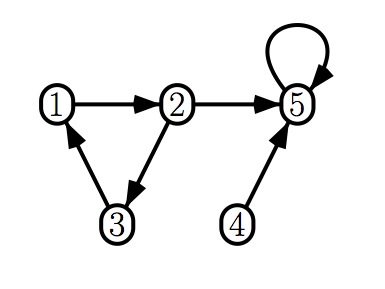
\includegraphics[scale=0.6]{img/RelationGraph}
\end{center}

\subsubsection{Seznamem seznamů}
Další způsob reprezentace pro uložení binární relace $R$ na množině $X$ (pro uložení binární relace v paměti počítače) je reprezentace seznamem seznamů. Tuto reprezentaci tvoří hlavní (spojový) seznam, ve kterém jsou uloženy všechny prvky množiny $X$. Z každého prvku $x \in X$ hlavního seznamu vede seznam obsahující právě ty $y \in X$, pro které platí $\langle x, y \rangle \in R$. Mějme relaci $R = \{\langle a, b\rangle,\langle a, d\rangle,\langle c, a\rangle,\langle b, d\rangle\}$ na množině $X = \{a,b,c,d\}$ potom reprezentace seznamem seznamů vypadá následovně.

\begin{center}
	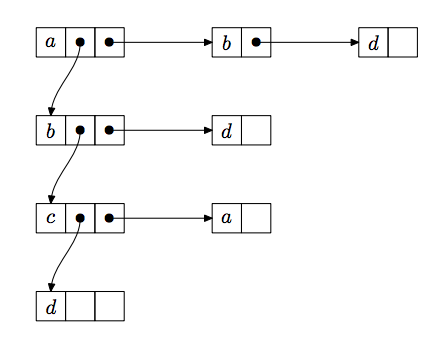
\includegraphics[scale=0.6]{img/RelationList}
\end{center}

\subsection{Zobrazení (funkce)}
Zobrazení (funkce) je matematickým protějškem běžně používaného pojmu přiřazení.

\begin{definition}
	Relace R mezi X a Y se nazývá zobrazení (funkce) množiny X do množiny Y, právě když pro každé $x \in X$ existuje právě jedno $y \in Y$ tak že $\langle x, y \rangle \in R$.
\end{definition}

\begin{definition}
	Zobrazení $f : X \rightarrow Y$ se nazývá
	\begin{itemize}
		\item[a)] \textbf{prosté (injektivní)}, právě když pro každé $x_1,x_2 \in X$, pro $x_1 \not= x_2$ plyne $f(x_1) \not= f(x_2)$,
		\item[b)] \textbf{surjektivní} nebo-li zobrazení X \textbf{na} Y, právě když pro každé $y \in Y$ existuje $x \in X$ tak, že  $f(x) = y$,
		\item[c)] \textbf{vzájemně jednoznačné (bijektivní)}, právě když je prosté a na (je tedy injektivní a současně surjektivní).
	\end{itemize}
\end{definition}

\begin{sentence}
	Pro zobrazení $f : X \rightarrow Y, g : Y \rightarrow Z$ platí
	\begin{itemize}
		\item[a)] $f \circ g$ je zobrazení,
		\item[b)] jsou-li f,g injekce, je $f \circ g$ injekce,
		\item[c)] jsou-li f,g surjekce, je $f \circ g$ surjekce.
	\end{itemize}
\end{sentence}

\begin{sentence}
	Nechť $f: A \rightarrow B$ je zobrazení. Inverzní relace $f^{-1}$ je zobrazením $B \rightarrow A$ tehdy a jen tehdy, je-li $f$ bijekce.
\end{sentence}

\begin{result}
	Nechť $f: A \rightarrow B, \ g: B \rightarrow C$ jsou bijekce. Pak
	\begin{itemize}
		\item[a)] $f^{-1} : B \rightarrow A$ je bijekce
		\item[b)] $g^{-1} \circ f^{-1}$ je bijekce C na A a platí $(f \circ g)^{-1} = g^{-1} \circ f^{-1}$.
	\end{itemize}
\end{result}

\begin{definition}
	Nechť $A \not= \emptyset$ je množina. Zobrazení $id_A : A \rightarrow A$ dané předpisem $id_A(x) = x$ pro každé $x \in A$ se nazývá \textbf{identické zobrazení}.
\end{definition}

\begin{sentence}
	Nechť $f : A \rightarrow B$ je zobrazení. Pak
	\begin{itemize}
		\item[a)] $f = f \circ id_B = id_A \circ f$
		\item[b)] $f$ je bijekce tehdy a jen tehdy, když existuje zobrazení $g : B \rightarrow A$ tak, že $f \circ g = id_A, g \circ f = id_B$
	\end{itemize}
\end{sentence}


\subsubsection{Poznámka k nekonečným množinám}
\begin{definition}
	Množina A se nazývá \textbf{spočetná} , právě když existuje bijekce $f : A \rightarrow \mathbb{N}$. Množina se nazývá \textbf{nespočetná}, právě když je nekonečná a není spočetná.
\end{definition}

\subsection{Binární relace na množině}
Binární relace na množině jsou matematickým protějškem vztahů mezi dvěma prvky množiny například: \uv{$x$ je menší než $y$}. Speciálními relacemi jsou \textbf{prázdná relace $\emptyset$, relace identity} $\omega_X = \{ \langle x, x \rangle \ | \ x \in X \}$, a \textbf{kartézský čtverec} $\tau_X = X \times X$.

\begin{definition}
Nechť $R$ je binární relace na $X$. Řekněme že $R$ je
\begin{itemize}
	\item \textbf{reflexivní}, pokud pro každé $x \in X$ platí $\langle x, x \rangle \in R$
	\item \textbf{symetrická}, pokud pro každé $x,y \in X$ platí $\langle x, y \rangle \in R \Rightarrow \langle y, x \rangle \in R$
	\item \textbf{antisymetrická}, pokud pro každé $x,y \in X$ platí \\$(\langle x, y \rangle \in R \wedge \langle y, x \rangle \in R) \Rightarrow x = y$
	\item \textbf{tranzitivní}, pokud pro každé $x,y,z \in X$ platí \\$(\langle x, y \rangle \in R \wedge \langle y, z \rangle \in R) \Rightarrow \langle x, z \rangle \in R$
	\item \textbf{irreflexivní}, pokud pro každé $x \in X$ platí $\langle x,x \rangle \not\in R$
	\item \textbf{asymetrická}, pokud pro každé $x,y \in X$ platí $\langle x, y \rangle \in R \Rightarrow \langle y, x \rangle \not\in R$
	\item \textbf{úplná}, pokud pro každé $x,y \in X$ platí $\langle x, y \rangle \in R \vee \langle y, x \rangle \in R$
\end{itemize}
\end{definition}

Relace $R$ je \textbf{(relace) ekvivalence}, jestliže je reflexivní, symetrická, a tranzitivní. Relace $R$ je \textbf{(relace) uspořádání}, jestliže je reflexivní, anti\-symetrická a tranzitivní.

\paragraph{Reflexivita} relace $R$ vyjadřuje, že každý prvek $x \in X$ je v relace \uv{sám se sebou}. V matici takovou relaci poznáme že má na diagonále samé 1, v orientovaném grafu je u každého uzlu smyčka.

\paragraph{Symetrie} relace $R$ vyjadřuje, že $\langle x, y \rangle \in R$ právě když  $\langle y, x \rangle \in R$ Tedy relace $R$ je symetrická pokud pro $\forall x,y \in X$ máme buď současně $\langle x, y \rangle \in R$ a  $\langle y, x \rangle \in R$, nebo současně  $\langle x, y \rangle \not\in R$ a  $\langle y, x \rangle \not\in R$. Symetrickou relaci v matici $M_R$ poznáme tak, že je symetrická podle hlavní podle hlavní diagonály. V grafu se tato relace pozná tak že pokud vede orientovaná hrana z $x$ do $y$ pak musí vést i z $y$ do $x$, nebo z $x$ do $y$ nevede žádná hrana.

\paragraph{Antisymetrie} relace $R$ vyjadřuje,že pro každé dav různé prvky $x,y \in X$ neplatí současně $\langle x, y \rangle \in R$ a  $\langle y, x \rangle \in R$. V matici $M_R$ poznáme antisymetrii tak, že dvě různá pole, která jsou souměrná podle diagonály neobsahují dvě jedničky. V grafu se antisymetrie projevuje tak, že meze dvěma různými vrcholy $x,y$ je buď jedna hrana nebo žádná.

\paragraph{Tranzitivita} relace $R$ vyjadřuje, že pro pokud $\langle x, y \rangle \in R$ a pokud $\langle y, z \rangle \in R$, pak také $\langle y, z \rangle \in R$. V grafu je tranzitivita projevuje tak, že pokud vede hrana z $x$ do $y$ a zároveň z $y$ do $z$ potom také $x$ do $z$.

\paragraph{Irreflexivita} relace $R$  vyjadřuje, že žádný prvek $x \in X$ není v relaci \uv{sám se sebou}.
\paragraph{Asymetrie} relace $R$  vyjadřuje, že do $R$ nepadnou $\langle x, y \rangle$ a  $\langle y, x \rangle$ současně.
\paragraph{Úplnost} relace $R$  vyjadřuje, že aspoň jedna z dvojic $\langle x, y \rangle$, $\langle y, x \rangle$ padne do $R$.

\subsection{Uzávěry relací}
Ke každé binární relaci můžeme stanovit její reflexivní, symetrický a tranzitivní uzávěr, to je nejmenší reflexivní, symetrickou a tranzitivní relaci na dané množině, která obsahuje výchozí relaci.

\begin{sentence}
	Nechť R je binární relace na X. Pak
	\begin{itemize}
		\item Ref(R) = $R \cup \omega_X$
		\item Sym(R) = $R \cup R^{-1}$
		\item Tra(R) = $\bigcup^\infty_{n=1} R^n$, kde $R^1 = R$ a $R^n = R \circ R^{n-1}$
	\end{itemize}
\end{sentence}

\subsection{Ekvivalence}
Je binární relace, kterou lze interpretovat jako matematický protějšek nerozlišitelnosti. Pro ekvivalenci $E$ na množině $X$ definujeme pro každý $x \in X$ množinu $[x]_E = \{ y \in X \ | \ \langle x, y \rangle \in E\} $
, kterou nazýváme \textbf{třída ekvivalence prvku} x. Zřejmě $[x]_E$ obsahuje právě ty prvky z $X$, které nelze od $x$ rozlišit ekvivalencí $E$.

\subsection{Rozklad}
Rozklad na množině je matematický protějšek shluků nerozlišitelných prvků. Rozklad na $X$ je \textbf{disjuktní pokrytí} $X$.

\begin{definition}
	Nechť $X \not= \emptyset$. Systém množin $\sqcap \subseteq 2^X$ splňující
	\begin{enumerate}
		\item $Y \not= \emptyset$ pro každou $Y \in \sqcap$,
		\item pro každé $Y_1,Y_2 \in \sqcap$ platí: pokud $Y_1 \cap Y_1 \not= \emptyset$, pak $Y_1 = Y_2$,
		\item $\bigcup\sqcap = X$,
	\end{enumerate}
	se nazývá \textbf{rozklad na množině} X. Množiny $Y \in \sqcap$ nazýváme \textbf{třídy rozkladu} $\sqcap$. Pro prvek $x \in X$ označíme $[x]_\sqcap$ tu třídu rozkladu $\sqcap$, která obsahuje x.
\end{definition}
Na množině $X$ existuji dva mezní rozklady.Prvním z nic je rozklad $\sqcap$, kde $[x]_\sqcap = \{x\}$ pro každé $x \in X$, tj všechny třídy rozkladu $\sqcap$ jsou jednoprvkové. Druhým mezním případem je rozklad $\sqcap = \{X\}$, tj. $\sqcap$ obsahuje jedinou třídu, která je rovna celé $X$, tedy $[x]_\sqcap = X$ pro každé $x \in X$.

\begin{sentence}
	Nechť $\sqcap$ je rozklad na X. Pak binární relace $E_\sqcap$ na X definovaná $\langle x,y \rangle \in E_\sqcap$, právě když $[x]_\sqcap = [y]_\sqcap$ je ekvivalence.
\end{sentence}

Kromě ekvivalencí a rozkladů existují další přirozené pohledy na to \uv{jak zjednodušit nazírání} na výchozí množinu. Jedním z nich je \textbf{surjektivní zobrazení}. Pokud je zobrazení $f : X \rightarrow Y$ surjektivní, pak lez chápat obraz $f(x)$ prvku $x$ jako vyjádření \uv{prvek $x$ nahradíme prvkem $f(x)$}. Ukážeme, že surjektivní zobrazení a ekvivalence mají zvláštní vztah. Pro zobrazení $f : X \rightarrow Y$ definujeme binární relaci $E_f$ na $X$ předpisem $$\langle x , y \rangle \in E_f \qquad \text{právě když} \qquad f(x) = f(y)$$
Zřejmě $E_f$ je ekvivalence, tzv. \textbf{ekvivalence indukovaná zobrazením} $f$.

\subsection{Uspořádání}
Uspořádání je v informatice zcela zásadní ačkoliv si to někdy neuvědomujeme, Mezi základní každého informatika patří znalost problému třídění a typických třídicích algoritmů. Problém třídění jako takový však de facto nemá smysl uvažovat pokud bychom na množině klíčů, podle kterých třídíme, nezavedli nějakou smysluplnou relaci uspořádání -- obvykle ji však chápeme jako \uv{určenou daným kontextem} a explicitně ji nezdůrazňujeme. Uspořádání množin může výrazně zvýšit efektivitu některých algoritmů, například vyhledávání.

\begin{definition}
	Reflexivní, antisymetrická a tranzitivní binární relace R na X se nazývá \textbf{uspořádání}. Úplné uspořádání se nazývá \textbf{lineární uspořádání} neboli \textbf{řetězec}. Pokud je R uspořádání na X, pak se $\langle X, R \rangle$ nazývá \textbf{upořádáná množina}.
\end{definition}

Relace uspořádání na $X$ obvykle značíme $\leq$ v souladu s intuitivním chápáním uspořádání a místo $\langle x ,y \rangle \in \ \leq$. Zdůrazněme ale, že označení $\leq$ v tuto chvíli nemá (obecně) nic společného se srovnáváním čísel, na které jsme zvyklí. Uspořádání pořád ještě není formálním protějškem \uv{upořádání} na které jsme zvyklí při porovnávání čísel. Je-li $\langle X, \leq \rangle$ uspořádaná množina, pak mohou  existovat $x,y \in X$ ,pro které neplatí $x \leq y$ ani $y \leq x$ (definice to nevylučuje). V tom případě říkáme, že prvky jsou \textbf{nesrovnatelné} což někdy značíme $x\ \| \ y$. V opačném případě prvky nazýváme \textbf{srovnatelné}. Je-li $\leq$ lineární uspořádání na $X$, pak je $\leq$ úplná relace, což znamená, že každé prvky jsou srovnatelné. Lineární uspořádání lze tedy chápat jako matematický protějšek \uv{tradičního srovnávání čísel}. Každá relace identity $\omega_X$ je uspořádání které nazýváme \textbf{antiřetězec}

\begin{sentence}
	Princip duality. Nechť $\leq$ je uspořádání na $X$. Pak $\leq^{-1}$ je uspořádání na $X$, které označujeme $\geq$.
\end{sentence}

Konečné uspořádání $\leq$ na $X$ je relace, mžeme ji tedy reprezentovat binární maticí nebo příslušným orientovaným grafem. Díky speciálním vlastnostem konečných uspořádání je však můžeme znázorňovat mnohem přehledněji pomocí speciálních diagramů. Ke každému uspořádání $\leq$ na $X$ lze uvažovat odvozenou relaci $\prec$ definovanou předpisem
$$x \prec y, \text{ právě když } x \leq y \text{ a } \forall z \in X \text{ platí: }$$
$$\text{pokud } x \leq z \leq y, \text{ pak } z \in \{ x, y\}$$



Relaci $\prec$ nazýváme pokrytí příslušné $\leq$ , a výraz $x \prec y$ čteme \uv{x je pokryt y} nebo \uv{x pokrývá y}. Na relaci pokrytí je založena jedna z metod jak znázornit konečnou uspořádanou množinu, tak zvané \textbf{Hasseovy diagramy} uspořádaných množin.

\begin{center}
	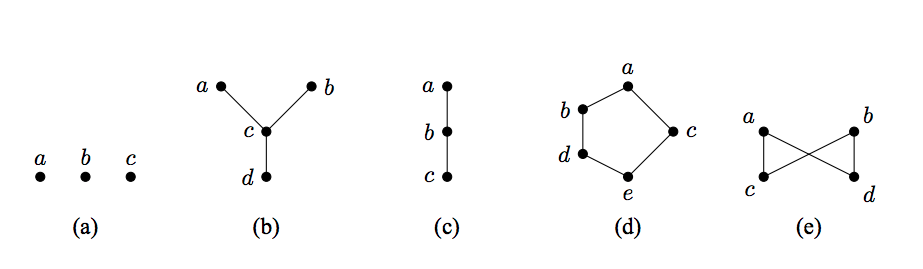
\includegraphics[width=12cm]{img/HasseDiagrams}
\end{center}

\begin{definition}
	Nechť $\langle X, \leq \rangle$ je uspořádaná množina. Prvek $x \in X$ se nazývá
	\begin{itemize}
		\item \textbf{minimální}, jestliže $\forall y \in X$ platí: pokud $y \leq x$, pak $x = y$,
		\item \textbf{nejmenší}, jestliže $x \leq y$ pro každá $y \in X$,
		\item \textbf{maximální}, jestliže $\forall y \in X$ platí: pokud $y \geq x$ pak $x = y$,
		\item \textbf{nejmenší}, jestliže $x \geq y$ pro každý $y \in X$.
	\end{itemize}
\end{definition}

\begin{sentence}
	Nechť $\langle X, \leq \rangle$ je uspořádaná množina. Pak platí
	\begin{enumerate}
		\item v $\langle X, \leq \rangle$ existuje nejvýše jeden největší a nejvýše jeden nejmenší prvek;
		\item je-li $x \in X$ největší (nejmenší) prvek, pak je také maximální (minimální);
		\item pokud je $\leq$ lineární uspořádání, pak je $x \in X$ největší (nejmenší) prvek, právě když je maximální (minimální).
	\end{enumerate}
\end{sentence}

\begin{definition}
	Nechť $\langle X, \leq \rangle$ je uspořádaná množina a nechť $Y \subseteq X$. Definujeme množiny
	$$L(Y) = \{ x \in X \ | \ x \leq y \text{ platí pro každé } y \in Y\}$$
	$$U(Y) =  \{ x \in X \ | \ x \geq y \text{ platí pro každé } y \in Y\}$$
	L(Y) se nazývá \textbf{dolní kužel množiny} Y v  $\langle X, \leq \rangle$. U(Y) se nazývá \textbf{horní kužel množiny} Y v  $\langle X, \leq \rangle$.
\end{definition}

Jinými slovy dolní kužel množiny $Y$ v  $\langle X, \leq \rangle$ obsahuje tedy právě ty prvky z $X$, které jsou menší nebo rovny všem prvkům obsaženým v $Y$, analogicky pro horní kužel.

\begin{definition}
	Nechť  $\langle X, \leq \rangle$ je uspořádaná množina a nechť $Y \subseteq X$. Pokud má $L(Y)$ největší prvek, pak se nazývá \textbf{infimum} Y a označuje se $inf(Y)$. Pokud má $U(Y)$ nejmenší prvek, pak se nazývá \textbf{supremum} Y a označuje se $sup(Y)$.
\end{definition}

\begin{definition}
	Nechť  $\langle X, \leq \rangle$ je uspořádaná množina. Pokud pro každé $x,y \in X$ existuje $inf(x,y)$, pak  $\langle X, \leq \rangle$ nazveme \textbf{průsekový polosvaz}. Pokud pro každé $x,y \in X$ existuje $sup(x,y)$ pak  $\langle X, \leq \rangle$ nazveme \textbf{spojový polosvaz}. Je-li  $\langle X, \leq \rangle$ průsekový i spojový polosvaz, pak  $\langle X, \leq \rangle$ nazveme \textbf{svaz}.
\end{definition}

\newpage
% ---------------------------------------------------------------------------------------------------------
% --------------------------------------------- druhý odstavec ---------------------------------------------
% ---------------------------------------------------------------------------------------------------------
\textbf{Vektorové prostory, lineární závislost a nezávislost, báze a dimenze vektorového prostoru. Eukleidovské vektorové
prostory. Matice, determinanty: vlastnosti, operace s nimi. Řešení soustav lineárních rovnic. Algebraické
struktury: grupa, okruh, obor integrity, těleso. Svazy: modulární, distributivní, komplementární.}

\section{Algebraické struktury}
\subsection{Grupoid}
\begin{definition}
	Nechť $A \not= \emptyset$. Binární operací na množině A nazveme každé zobrazení $f : A \times A \rightarrow A$.
\end{definition}

\begin{example}
	Nechť $\mathbb{Z}$ je množina všech celých čísel, + přiřadí každé dvojici čísel $a,b \in \mathbb{Z}$ číslo $a + b \in \mathbb{Z}$. Je tedy binární operace.
\end{example}

\begin{definition}
	Nechť $A \not= \emptyset$ a $\circ$ je binární operace na A. Dvojici $\mathscr{A} = (A, \circ)$ budeme nazývat grupoid. Jeli operace $\circ$ asociativní, tj. jestliže $\forall a,b,c \in A$ platí $a \circ (b \circ c) = (a \circ b) \circ c$, nazývá se grupoid $(A, \circ)$ pologrupa. Operace $\circ$ se nazývá komutativní jestliže $a \circ b = b \circ a$ pro každé $a,b \in A$.
\end{definition}

Budeme-li operaci v grupoidu zapisovat symbolem +, nazýváme grupoid $(A, +)$ \textbf{aditivní}, budeme-li operaci zapisovat $\circ$ (nebo vynechávat), nazývá se grupoid $(A, \circ)$ \textbf{multiplikativní}.

\begin{definition}
	Jestliže v grupoidu $(A, \circ)$ existuje prvek $e$ takový, že $a \circ e = e \circ a = a$ pro každé $a \in A$, nazývá se e \textbf{jednotkou} $(A, \circ)$. Jestliže v A existuje prvek n takový, že $a \circ n = n \circ a = n$, nazývá se n \textbf{nula} grupoidu $(A, \circ)$.
\end{definition}

\begin{definition}
	Nechť $\mathscr{A} = (A, \circ)$ je grupoid, nechť $\emptyset \not= B \subseteq A$.Jestliže $\forall a,b \in B$ platí $a \circ b \in B$, nazývá se $(B, \circ)$ \textbf{podgrupoid} grupoidu $\mathscr{A}$.
\end{definition}

\subsection{Grupa}
\begin{definition}
	Nechť $(A, \circ)$ je pologrupa. Jestliže pro každé dva prvky $a,b \in A$ existují $x,y \in A$ tak, že platí  $a \circ x = b, y \circ a = b$, pak se $(A, \circ)$ se nazývá \textbf{grupa}.
\end{definition}

Další možností jak definovat to, že je grupoid $\mathscr{G}$ grupa říká následující definice.
\begin{definition}
	 $\mathscr{G} = (G, \circ)$  nazveme grupou pokud platí
	\begin{enumerate}
		\item $\forall a,b, \in G : a \circ b \in G$ (uzavřenost)
		\item $\forall a,b,c \in G : (a \circ b) \circ c = a \circ (b \circ c)$ (asociativita)
		\item $\exists e \in G \quad \forall a \in G : a \circ e = e \circ a = a$ (jednotkový prvek)
		\item $\forall a \in G \quad \exists a^{-1} \in G : a \circ a^{-1} = a^{-1} \circ a = e$ (inverzní prvek)
	\end{enumerate}
	Grupa se nazývá \textbf{abelovská} právě když platí komutativita: $$\forall a,b, \in G : a \circ b = b \circ a$$
\end{definition}

\begin{definition}
	Nechť $\mathscr{G} = (G, \circ)$ je grupa. Podgrupoid $(A, \circ)$ grupoidu $(G, \circ)$ se nazývá \textbf{podgrupa grupy} $\mathscr{G}$, je-li $(A, \circ)$ grupou.
\end{definition}

\begin{example}
	Grupa $(\mathbb{Z}, +)$ je podgrupou grupy $(\mathbb{R}, +)$ všech reálných čísel.
\end{example}

\subsection{Okruh}
\begin{definition}
	\textbf{Okruhem} nazveme trojici $\mathscr{R} = (R, + , \cdot)$ takovou, že $R \not= \emptyset$ je množina, + a $\cdot$ jsou binární operace na R a
	\begin{enumerate}
		\item $(R, +)$ je abelovská grupa (0 její jednotka)
		\item $(R, \cdot)$ je pologrupa
		\item Platí \textbf{distributivní zákony}, tj. pro každé $a,b,c \in R$ platí $$a \cdot (b + c) = a \cdot b + a \cdot +\ c, \qquad (b + c) \cdot a = b \cdot a + c \cdot a$$
	\end{enumerate}
	Okruh $\mathscr{R}$ se nazývá \textbf{komutativní}, jestliže $ a \cdot b = b \cdot a$ pro každé $a,b \in R$. Okruh $\mathscr{R}$ se nazývá \textbf{unitární}, má-li pologrupa $(R \setminus \{0\}, \cdot)$ jednotku. Je-li $\mathscr{R}$ unitární, budeme jeho jednotku označovat 1. Prvek 0 (jednotka $(R, +)$) se nazývá \textbf{nulou okruhu} $\mathscr{R}$.
\end{definition}

\begin{example}
	Komutativní unitární okruhy jsou například: okruh celých čísel $(\mathbb{Z}, + , \cdot)$, okruh reálných čísel $(\mathbb{R}, + , \cdot)$, okruh komplexních čísel $(\mathbb{C}, + , \cdot)$ a okruh racionálních čísel $(\mathbb{Q}, + , \cdot)$.
\end{example}

\begin{definition}
	Prvek a okruhu $\mathscr{R} = (R,+,\cdot)$ se nazývá \textbf{dělitel nuly}, jestliže $a \not= 0$ existuje $b \not= 0, b \in R$ tak, že $a \cdot b = 0$.
\end{definition}

\subsection{Obor integrity}
\begin{definition}
	Okruh $\mathscr{R} = (R,+,\cdot)$ se nazývá \textbf{obor integrity}, je-li komutativní, unitární a neobsahuje dělitele nuly.
\end{definition}

\begin{example}
	Každý z okruhů $(\mathbb{Z}, + , \cdot)$, $(\mathbb{R}, + , \cdot)$,  $(\mathbb{C}, + , \cdot)$, $(\mathbb{Q}, + , \cdot)$ je obor integrity.
\end{example}


\subsection{Těleso}
\begin{definition}
	Okruh $\mathscr{R} = (R,+,\cdot)$ se nazývá \textbf{těleso}, je-li množina jeho nenulových prvků grupou vzhledem k operaci $\cdot$. Těleso $\mathscr{R}$ se nazývá \textbf{komutativní}, je-li $(R \setminus \{0\}, \cdot)$ abelovská grupa.
\end{definition}

\begin{example}
	Okruhy  $(\mathbb{R}, + , \cdot)$,  $(\mathbb{C}, + , \cdot)$, $(\mathbb{Q}, + , \cdot)$ jsou komutativní tělesa. Okruh $(\mathbb{Z}, + , \cdot)$ není těleso.
\end{example}

\begin{sentence}
	Každé komutativní těleso je obor integrity.
\end{sentence}

\begin{definition}
	Je-li  $\mathscr{R} = (R,+,\cdot)$ okruh, $A \subseteq R$ taková že  $(A,+,\cdot)$ je opět okruh, pak se    $(A,+,\cdot)$ nazývá \textbf{podokruh okruhu} $\mathscr{R}$. Je-li  $\mathscr{R} = (R,+,\cdot)$ těleso, $A \subseteq R$ taková že  $(A,+,\cdot)$ je opět těleso, pak se $(A,+,\cdot)$ nazývá \textbf{podtěleso tělesa} $\mathscr{R}$. Každé podtěleso tělesa $\mathscr{C} = (C,+,\cdot)$  komplexních čísel nazveme \textbf{číselné těleso}. Každý podokruh okruhu  $\mathscr{C}$ nazveme \textbf{číselný okruh}.
\end{definition}

\begin{example}
	 $ \mathscr{R} = (\mathbb{R}, + , \cdot)$,  $\mathscr{C} = (\mathbb{C}, + , \cdot)$, $ \mathscr{Q} = (\mathbb{Q}, + , \cdot)$ jsou číselná tělesa. $\mathscr{Z} = (\mathbb{Z}, + , \cdot)$ je číselný okruh, který není tělesem.
\end{example}

\section{Vektorové prostory}
\begin{definition}
	Nechť $A \not= \emptyset \not= B$ jsou množiny. Zobrazení $\circ : A \times B \rightarrow B$ nazveme \textbf{levá vnější operace nad množinami} A,B (v tomto pořadí). Jsou-li $a \in A, b \in B$, pak prvek $\circ(a,b)$ budeme zapisovat $a \circ b$.
\end{definition}

\begin{definition}
	Nechť $(V, +)$ je abelovská grupa, nechť T je číselné těleso, nechť $\circ : T \times V \rightarrow V$ je levá vnější operace nad T,V. Pak čtveřici $\mathscr{V} = (V, +, T, \circ)$ nazveme \textbf{vektorový prostor nad} T, platí-li $\forall u,v \in V, \forall c,d, \in T$
	\begin{enumerate}
		\item $c \circ (u + v) = c \circ u + c \circ v$
		\item $(c + d) \circ u = c \circ u + d \circ u$
		\item $(c \cdot d) \circ u = c \circ (d \circ u)$
		\item $1 \circ u = u$
	\end{enumerate}
	Prvky v V budeme nazývat \textbf{vektory}, čísla z tělesa T \textbf{skaláry}. Množinu V nazveme \textbf{pole} vektorového prostoru $\mathscr{V}$.
\end{definition}

\begin{definition}
	Nechť  $\mathscr{V}$ je vektorový prostor nad tělesem T, nechť $v,u_1,\dots,u_k \in V$. Řekneme, že vektor v je \textbf{lineární kombinací vektorů}  $v,u_1,\dots,u_k$, jestliže existují čísla $c_1, \dots, c_k \in T$ tak, že $$v = c_1 \cdot u_1 + \dots + c_k \cdot u_k$$
\end{definition}
\paragraph{Poznámka.} Symbolem \textbf{o} budeme označovat tzv. \textbf{nulový vektor}, což je jednotka grupy $(V, +)$. Použitím podmínky 2. dostaneme $\forall u \in V:$ $$0 \cdot u = (c + (-c)) \cdot u = c \cdot u + (-c \cdot u) = o$$
Tedy nulový vektor je lineární kombinací libovolných vektorů z $V: $ je-li $u_1,\dots,u_k \in V$ pak $$0 \cdot u_1 + \dots + 0 \cdot u_k = o$$


\begin{definition}
	Vektory $u_1, \dots, u_k$ z vektorového prostoru $\mathscr{V}$ se nazývají \textbf{lineárně závislé}, jestliže existují čísla $c_1, \dots, c_k \in T$, která nejsou všechna rovna nule tak, že nulový vektor \textbf{o} je roven netriviální lineární kombinaci vektorů $u_1, \dots, u_k$, tj. $$o = c_1 \cdot u_1 + \dots + c_k \cdot u_k,$$
	kde aspoň jedno $c_i \not= 0$. Jestliže vektory $u_1, \dots, u_k$ nejsou lineárně závislé, nazývají se \textbf{lineárně nezávislé}.
\end{definition}

\paragraph{Poznámka.} Zřejmě vektory  $u_1, \dots, u_k \in \mathscr{V}$ jsou lineárně nezávislé, právě když $$o = c_1 \cdot u_1 +  \dots + c_k \cdot u_k \quad \Rightarrow \quad c_1 = c_2 = \dots = c_k = 0$$

\begin{sentence}
	Jsou-li mezi vektory  $u_1, \dots, u_k \in \mathscr{V}$  některé lineárně závislé, pak jsou  $u_1, \dots, u_k$ lineárně závislé.
\end{sentence}

\begin{sentence}
	Je-li mezi vektory  $u_1, \dots, u_k$  vektor nulový \textbf{o}, pak jsou $u_1, \dots, u_k$ lineárně závislé.
\end{sentence}

\begin{sentence}
	Nechť $u_1, \dots, u_k \in \mathscr{V}$. Pak  $u_1, \dots, u_k$ jsou lineárně závislé, právě když je aspoň jeden z nich lineární kombinací ostatních vektorů.
\end{sentence}

\begin{definition}
	Nechť  $\mathscr{V} = (V, +, T, \circ)$  je vektorový prostor nad tělesem T, nechť $\emptyset \not= W \subseteq V$. Pak  $\mathscr{W} = (W, +, T, \circ)$ nazveme \textbf{podprostor vektorového prostoru} $\mathscr{V}$, jestliže
	\begin{enumerate}
		\item $\forall u,c \in W$ je $u + v \in W$
		\item $\forall u \in W, \forall c \in T$ je $c \cdot u \in W$.
	\end{enumerate}
\end{definition}


\begin{definition}
	nechť M je podmnožina vektorového prostoru $\mathscr{V}$. \textbf{Lineárním obalem množiny M ve} $\mathscr{V}$ rozumíme množinu všech lineárních kombinací vektorů z M.
\end{definition}

\begin{definition}
	Nechť  $\mathscr{V}$ je vektorový prostor, $M \not= \emptyset$ jeho podmnožina. Je-li $[M] =\mathscr{V}$, nazývá se M množina generátorů  $\mathscr{V}$.
\end{definition}

\begin{definition}
	Řekněme, že vektorový prostor $\mathscr{V}$ je konečné dimenze, má-li aspoň jednu konečnou množinu generátorů.
\end{definition}

\begin{definition}
	Bází vektorového prostoru $\mathscr{V}$ konečné dimenze rozumíme libovolnou lineárně nezávislou konečnou množinu $\{u_1, \dots, u_n\}$ jeho generátorů.
\end{definition}

\begin{sentence}
	Nechť $M = \{u_1, \dots, u_n\}$ je bází $\mathscr{V}$. Pak každý vektor $v \in \mathscr{V}$ lze jediným způsobem vyjádřit jako lineární kombinaci vektorů $u_1, \dots, u_n$.
\end{sentence}

\begin{example}
	Příklad báze vektorového prostoru $e_1 = (1,0,0,0), e_2 = (0,1,0,0), e_3 = (0,0,1,0), e_4 = (0,0,0,1)$
\end{example}

\begin{definition}
	Je-li $\mathscr{V} \not= \{o\}$  vektorový prostor konečné dimenze, pak počet prvků jeho libovolné báze nazýváme dimenze $\mathscr{V}$ a značíme $dim\mathscr{V}$, Je-li $\mathscr{V} = \{o\}$, položíme dim$\mathscr{V} = 0$.
\end{definition}


\subsection{Aritmetické vektorové prostory}
Nechť $T$ je číselné těleso, $n$ přirozené číslo. Na n-násobném kartézském součinu $T^n = V$ definujeme operaci $+$ takto: je-li $(a_1,a_2,\dots, a_n), (b_1,b_2,\dots, b_n) \in V$ pak $$(a_1,a_2,\dots, a_n) +(b_1,b_2,\dots, b_n) = (a_1 + b_1, a_2 + b_2,\dots, a_n + b_n).$$
Zřejmě $(V, +)$ je abelovská grupa, prvek $o = (0,0, \dots, 0)$ je její jednotkou a prvek $(- a_1, \dots, - a_n)$ je inverzní k prvku $(a_1, \dots, a_n)$. Definujeme levou vnější operaci: $c \in T, (a_1, \dots, a_n) \in V$, $$c \cdot (a_1,\dots, a_n) = (c \cdot a_1,\dots,c \cdot a_n).$$

Jednoduše lze ověřit, že $\mathscr{V} = (V,+,T,\cdot)$ je vektorový prostor dimenze $n$. Tento vektorový prostor nazveme aritmetický a budeme jej značit $T^n$. Jednou z jeho (nekonečně mnoha) bází je $e_1, \dots, e_n)$, kde $e_1 = (1,0,\dots, 0),\ e_2 = (0,1,\dots, 0),\ \dots, \ e_n = (0,0,\dots, 1)$ 

Zapisujeme-li aritmetický vektor \textbf{a} ve tvaru $(a_1,a_2, \dots, a_n)$, nazýváme tento zápis \textbf{řádkový vektor}. zapisujeme-li \textbf{a} ve tvaru 
\begin{displaymath}
	a = \left( 
	 \begin{array}{c}
		a_1\\ a_2 \\ \vdots \\ a_n
	\end{array}\right)
\end{displaymath}
nazýváme jej sloupcový vektor.
\subsection{Eukleidovské vektorové prostory}
Ve vektorovém prostoru nad tělesem $T$ můžeme vektory sčítat, odčítat a násobit skaláry z tělesa $T$ (levá vnější operace). Nemáme však zaveden pojem délky vektoru, úhlu mezi vektory apod. Zavedeme proto další pojem.

\begin{definition}
	Nechť $\mathscr{V} = (V, +, \mathbb{R}, \cdot)$ je vektorový prostor nad tělesem reálných čísel $\mathbb{R}$. \textbf{Skalárním součinem} $\circ$ nazveme zobrazení $V \times V$ do tělesa $\mathbb{R}$, které má tyto vlastnosti:
	\begin{enumerate}
		\item $\forall u,v \in V, u \circ v = v \circ u$
		\item $\forall u \in V, u \not= o, u \circ u > 0$
		\item $\forall u,v,w \in V, (u + v) \circ w = u \circ w + v \circ w$
		\item $\forall u,v \in V, \forall c \in \mathbb{R}, (c \cdot u) \circ v = c \cdot (u \circ v)$.
	\end{enumerate}
\end{definition}

\begin{example}
	Je-li $\mathscr{V} = (\mathbb{R}^n, +, \mathbb{R}, \cdot)$ aritmeticky (n-dimenzionální) vektorový prostor nad $\mathbb{R}, x = (x_1,x_2, \dots, x_n), y = (y_1,y_2, \dots, y_n)$, pak $x \circ y = \sum^n_{i=1} x_i \cdot y_i$ definuje skalární součin $\circ$.
\end{example}

\begin{definition}
	Nechť $\mathscr{V} = (V, + \mathbb{R}, \cdot)$ je vektorový prostor nad tělesem reálných čísel, ve kterém je definován skalární součin. Pak se $\mathscr{V}$ nazývá \textbf{Eukleidovský vektorový prostor}
\end{definition}

\begin{definition}
	Nechť $\mathscr{V}$ je Eukleidovský vektorový prostor, nechť $u \in V$. Číslo $\| u \| = \sqrt{u \circ u}$ nazveme délka vektoru u.
\end{definition}

\begin{definition}
	Nechť $\mathscr{V}$ je Eukleidovský vektorový prostor, $u,v \in V$. Pak
	\begin{itemize}
		\item[a)] $\forall c \in \mathbb{R}$ je $\| c \cdot u \| = |c| \cdot \| u \|$
		\item[b)] $\| o \|$ a pro $u \not= o$ je $\| u \| > 0$
		\item[c)] $|u \circ v| \leq \| u \| \cdot \| v \|$ (Schwarzova nerovnost)
	\end{itemize}
\end{definition}

\begin{definition}
	Nechť $\mathscr{V}$ je Eukleidovský vektorový prostor, $u,v \in V$, $u \not= o \not= v$. Úhlem $\varphi$ vektorů u,v nazveme číslo $$\varphi = arccos \frac{u \circ v}{\| u \| \cdot \| v \|}$$
\end{definition}
Platí tedy $cos \varphi = \frac{u \circ v}{\| u \| \cdot \| v \|}$, kde $0 < \varphi < \pi$

\begin{definition}
	Vektory u,v nazveme ortogonální (kolmé). ozn. $u \bot v$, je-li $\varphi = \frac{\pi}{2}$ tj. $cos \varphi = 0$, tj. $u \circ v = 0$.
\end{definition}

\begin{definition}
	Vektory $u_1, \dots, u_m$ jsou vzájemně ortogonální, platí-li $u_i \bot u_j$ pro každé $i \not= j$.
\end{definition}

\begin{sentence}
	Nenulové vzájemně ortogonální vektory $u_1, \dots, u_m$ jsou lineárně nezávislé.
\end{sentence}

\begin{definition}
	Jsou-li  $u_1, \dots, u_m$ vzájemně ortogonální vektory, přičemž $\{ u_1, \dots, u_m\}$ generuje celý prostor $\mathscr{V}$, pak je to báze $\mathscr{V}$ (tzv. ortogonální báze).
\end{definition}

\section{Matice}
\begin{definition}
	Nechť T je číselné těleso, m,n jsou čísla přirozená a nechť $a_{ij} \in T$  pro $i = 1, \dots, m, j = 1, \dots n.$ Dvojindexované schéma
\begin{displaymath}
{\bf A} =
\left( \begin{array}{cccc}
a_{11} & a_{12} & \dots & a_{1n} \\
a_{21} & a_{22} & \dots & a_{2n} \\
\vdots &  &  &  \\
a_{m1} & a_{m2} & \dots & a_{mn} \\
\end{array} \right)
\end{displaymath}
se nazývá matice typu $m \times n$ nad T. Číslo $a_{ij}$ se nazývá prvek matice A z i-tého řádku a j-tého sloupce. Číslo i se nazývá řádkový, číslo j sloupcový index prvku $a_{ij}$.
\end{definition}

\paragraph{Poznámka.} Někdy budeme matice značit následovně: $A = \| a_{ij}\|$.

\begin{definition}
	Matice $A = \|a_{ij}\|$ typu $m \times n$, kde $m = n$ se nazývá čtvercová matice stupně n. Čtvercová matice A se nazývá diagonální pokud pro všechny její prvky. která neleží na hlavní diagonále jsou rovny 0. Diagonální matice se nazývá skalární, jestliže všechny její prvky na hlavní diagonále jsou si rovny. Skalární matice se nazývá jednotková stupně n, jsou-li všechny její prvky na hlavní diagonále rovny 1 (budeme ji označovat $E_n$). Matici N typu $m \times n$ nazveme nulová matice jestliže jsou všechny její prvky rovny 0.
\end{definition}

\paragraph{Označení.} Symbolem $\mathscr{M}_{m \times n}(T)$ resp. $\mathscr{M}_{n}(T)$ označíme množinu všech matic typu $m \times n$ resp. všech čtvercových matic stupně $n$ nad tělesem $T$.

\begin{definition}
	Dvě matice $A,B$ z $\mathscr{M}_{m \times n}(T)$ jsou si rovny, jestliže $a_{ij} = b_{ij}$ pro každé  $i = 1, \dots, m, j = 1, \dots n.$
\end{definition}

\begin{definition}
	Mějme matice $A,B \in \mathscr{M}_{m \times n}(T)$. Součtem matice $A$ a $B$ rozumíme matici $A + B = \|c_{ij}\|$, kde $ \|c_{ij}\| =  a_{ij} + b_{ij}$ pro každé $i = 1, \dots, m, j = 1, \dots n.$
\end{definition}

\begin{sentence}
	Množina $\mathscr{M}_{m \times n}(T)$ spolu se zavedenou operací sčítání matic tvoří abelovskou grupu.
\end{sentence}
\begin{definition}
	Nechť T je číselné těleso, $A \in \mathscr{M}_{m \times n}(T)$. Prvky z T budeme nazývat skaláry. zavedeme levou vnější operaci $\cdot : T \times  \mathscr{M}_{m \times n}(T) \rightarrow \mathscr{M}_{m \times n}(T)$ takto: $c \in T, \ A= \| a_{ij} \| \ pak \ cA = \|c \cdot a_{ij} \|$ je tzv. násobení matice skalárem.
\end{definition}

\begin{definition}
	Nechť $A= \| a_{ij} \|$ je matice typu $m \times n$. Matici transponovanou k matici A nazýváme matici $A^T = \| a_{ji} \|$ typu $n \times m$ která vznikne z A vzájemnou výměnou řádků a sloupců (tj. otočením A podle hlavní diagonály).
\end{definition}

\begin{definition}
	Nechť $A= \| a_{ij} \|$ je matice typu $m \times n$ a nechť $B= \| b_{jk} \|$ je matice typu $n \times p$  nad tělesem T. Součinem matic A a B (v tomto pořadí) nazveme matici $AB =  \| c_{ik} \|$ typu $m \times p$ pro jejíchž prvky platí: $$c_{ik} = a_{i1}b_{1k} + a_{i2}b_{2k} + \dots + a_{in}b_{nk} = \sum^n_{j=1} a_{ij}b_{jk}$$
	pro každé $i = 1, \dots, m, k = 1, \dots p.$
\end{definition}

\begin{sentence}
	Násobení matic je asociativní, tj. jestliže $A \in \mathscr{M}_{m \times n}(T), B \in \mathscr{M}_{n \times p}(T), C \in \mathscr{M}_{p \times r}(T)$, pak $$(AB)C = A(BC).$$
\end{sentence}

\begin{sentence}
	Nechť T je těleso $n \in \mathbb{N}$. Pak $ \mathscr{M}_{n}(T) = (\mathscr{M}_{n}(T) ,+,\cdot)$ je unitární okruh, jehož jednotkou je jednotková matice. Je-li $n > 1$ pak tento okruh není komutativní a obsahuje dělitele nuly. Je-li $n = 1$ pak $\mathscr{M}_{1}(T)$  je komutativní těleso.
\end{sentence}

\section{Determinanty}

\subsection{Permutace}
\begin{definition}
Nechť $A = \{a_1,a_2, \dots, a_n\}$ konečná (n-prvková) množina. Pořadím $\pi$ množiny A nazveme libovolnou posloupnost $\pi = (a_{k_1},a_{k_2}, \dots, a_{k_n})$ prvků z A takovou, že každý prvek z A se v $\pi$ vyskytuje právě jedenkrát. Permutací na A rozumíme každou bijekci A na A. Permutaci P množiny A lze zapisovat ve tvaru
\begin{displaymath}
{\bf A} =
\left( \begin{array}{cccc}
a_{1} & a_{2} & \dots & a_{n} \\
a_{\pi (1)} & a_{\pi (2)} & \dots & a_{\pi (n)} \\

\end{array} \right)
\end{displaymath}
kde $\pi$ je některé pořadí množiny indexů.
\end{definition}

\begin{definition}
	Pro každou n-prvkovou množinu $(n \geq 1)$ je počet pořadí roven počtu permutací, tj. n!.
\end{definition}


\begin{definition}
	Nechť $\pi = \{k_1,k_2, \dots, k_n\}$ je pořadím množiny $A = \{ 1,2,\dots, n\}$. Prvky $k_i,k_j$ tvoří inverzi v $\pi$, jestliže $i < j$ a  $k_i > k_j$. Označme $[\pi]$ počet všech inverzí v $\pi$. Znaménkem pořadí $\pi$ nazveme číslo $sgn\pi = (-1)^{[\pi]}$. Je-li $sgn\pi = 1$, pořadí se nazývá sudé, je-li $sgn\pi = -1$,  $\pi$ se nazývá liché. Nechť $P = { \pi_1 \choose \pi_2}$ je permutace množiny A. Znaménkem permutace P rozumíme číslo sgnP, kde $sgnP = 1$ je-li $sgn\pi_1 = sgn\pi_2$, $sgnP = -1$, je-li $sgn\pi_1 = - sgn\pi_2$. Je-li $sgnP = 1$, P je sudá, je-li $sgnP = -1$, je P lichá.
\end{definition}

\begin{example}
	Nechť $\pi = (2,4,3,5,1)$. Pak všechny jeho inverze jsou: 2,1; 4,3; 4,1; 3,1; 5,1. Tedy $[\pi] = 5$ tj. $sgn\pi = (-1)^5 = -1$, $\pi$ je liché.
	Nechť ${\bf A} =
\left( \begin{array}{ccccc}
2 & 1 & 4 & 5 & 3 \\
4 & 3 & 1 & 2 & 5 \\
\end{array} \right) = \left( \begin{array}{c}
\pi_1 \\
\pi_2 \\
\end{array} \right) $. Ověříme $[\pi_1] = 3, [\pi_2] = 5$, tedy $sgn\pi_1 = -1 = sgn\pi_2$, odkud $sgnP = 1$, tj. P je sudá permutace.
\end{example}

\paragraph{Poznámka.} Je-li $P = \left( \begin{array}{c} \pi_0 \\ \pi_1 \\ \end{array} \right)$, kde $\pi_0$ je základní pořadí, pak zřejmě $sgnP = sgn\pi_1$

\paragraph{Označení.} Symbolem $P_0$ značíme \textbf{identickou permutaci}, tj. $P_0 = \left( \begin{array}{c} \pi_0 \\ \pi_0 \\ \end{array} \right)$. Je-li $P = \left( \begin{array}{c} \pi_1 \\ \pi_2 \\ \end{array} \right)$, symbolem $P^{-1}$ označíme \textbf{inverzní permutaci}, tj. $P^{-1} = \left( \begin{array}{c} \pi_2 \\ \pi_1 \\ \end{array} \right)$,

\begin{definition}
	\textbf{Transpozicí} na $A = \{1, \dots, n\}$ rozumíme permutaci P takovou, že existují $i,j \in A, i \not= j$ tak, že $P(i) = j, P(j) = i$ a $P(k) = k$ pro každé $i \not= k \not= j$.
\end{definition}

\begin{example}
	$P = \left( \begin{array}{cccccc} 1 & 2 & 3 & 4 & 5\\ 1 & 4 & 3 & 2 & 5 \\ \end{array} \right)$ je transpozice, zaměňuje 2 a 4.
\end{example}

\paragraph{Označení.} Transpozici $P$ zaměňující $i$ a $j$ budeme zapisovat $P(i,j)$.


\begin{sentence}
	Každou permutaci je možné vyjádřit jako složení konečného počtu transpozic. Permutace P je sudá (resp. lichá), je-li tento počet transpozic sudý (resp. lichý).
\end{sentence}

\subsection{Konečně co je to determinant}
\begin{definition}
	Nechť $A = \| a_{ij} \|$ je čtvercová matice stupně n nad číselným tělesem T. Determinantem detA matice A rozumíme číslo z T takové, že $$detA =  \sum_P sqnP \cdot a_{1k_1}a_{2k_2} \dots a_{nk_n},$$ kde sčítáme přes všechny permutace $P = \left( \begin{array}{cccc} 1 & 2 & \dots & n\\ k_1 & k_2 & \dots & n \\ \end{array} \right)$. Každý ze součinů \\$a_{1k_1}a_{2k_2} \dots a_{nk_n}$ nazýváme člen determinantu detA.
\end{definition}
Tedy determinant matice $A$ je číslo z $T$, které je rovno součtu všech $n!$ součinů prvků matice $A$, ke v každém součinu je každý prvek právě z jednoho řádku a právě z jednoho sloupce, přičemž součin je opatřen znaménkem rovným znaménku permutace určené řádkovými a sloupcovými indexy prvků tohoto součinu.

\begin{example}
	Určete determinant matice
	\begin{displaymath}
{\bf A} =
\left( \begin{array}{cc}
a_{11} & a_{12}  \\
a_{21} & a_{22}  \\
\end{array} \right)
\end{displaymath}
Jeho členy tedy budou součiny $a_{11}a_{22}, a_{12}a_{21}$ Určíme jejich znaménka:
	\begin{displaymath}
{\bf sgn} =
\left( \begin{array}{cc} 1 & 2  \\ 1 & 2  \\ \end{array} \right) = 1,\
{\bf sgn} = \left( \begin{array}{cc} 1 & 2  \\ 2 & 1 \\ \end{array} \right) = -1
\end{displaymath}
Tedy $$detA = a_{11}a_{22} - a_{12}a_{21}$$
\end{example}

\begin{sentence}
	Má-li čtvercová matice A v některém řádku (resp. sloupci) samé 0, je $detA = 0$.
\end{sentence}

\paragraph{Sarusovo pravidlo} pro výpočet determinantu matic maximálně 3-tého stupně. Mějme matici A druhého stupně $A = \left( \begin{array}{ccc} 5 & 3 & 2\\ 1 & 7 & -8\\ 0 & -2 & 7\\ \end{array} \right)$ použijeme následující schéma výpočtu: 
\begin{center}
	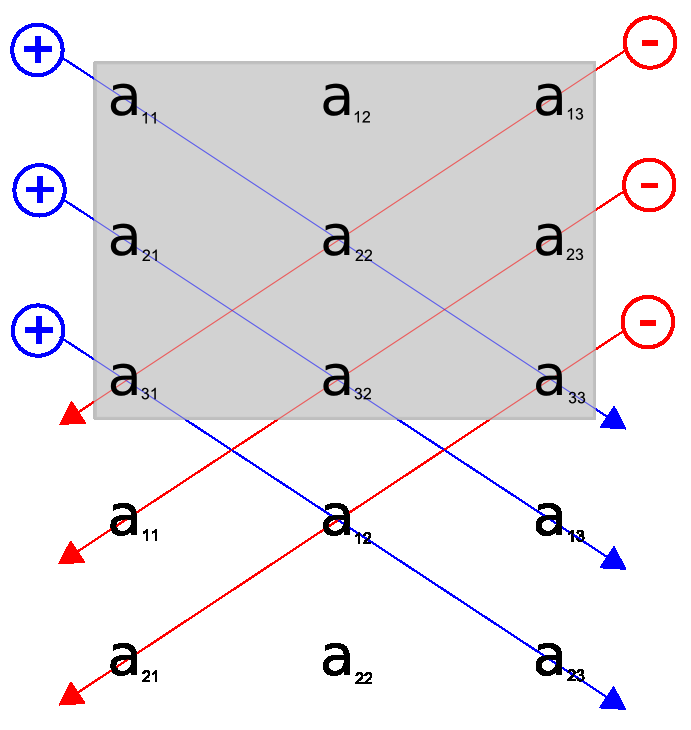
\includegraphics[scale=0.2]{img/SarussRule}
\end{center}
Naše \uv{rozšířená matice} bude vypadat následovně $A = \left( \begin{array}{ccc} 5 & 3 & 2\\ 1 & 7 & -8\\ 0 & -2 & 7\\ 5 & 3 & 2\\ 1 & 7 & -8\\ \end{array} \right)$ A determinant $detA = [5⋅7⋅7+1⋅(−2)⋅2+0⋅3⋅(−8)]−[2⋅7⋅0+(−8)⋅(−2)⋅5+7⋅3⋅1]=140$
\begin{sentence}
	Má-li $A \in \mathscr{M}_n(T)$ všechny prvky pod hlavní diagonálou rovny nule, pak $detA = a_{11}a_{22}\dots a_{nn}$. 
\end{sentence}

\begin{sentence}
	Vznikne-li matice B z matice $A \in \mathscr{M}_n(T)$ záměnou i-tého a j-tého řádku (resp. sloupce), přičemž $i \not= j$, pak $detB = - detA$.
\end{sentence}

\begin{sentence}
	Vznikne-li matice B z matice $A \in \mathscr{M}_n(T)$ provedením některé permutace P na řádky (resp. sloupce) matice A, pak $detB = sgnP \cdot detA$.
\end{sentence}

\begin{definition}
	Nechť $A = \| a_{ij} \| \in \mathscr{M}_{m \times n}(T)$. Pak každou matici, která vznikne z A vynecháním některých řádků a některých sloupců nazýváme dílčí matice A. Je-li dílčí matice matice A čtvercová, pak její determinant nazýváme subdeterminant A.
\end{definition}

\begin{definition}
	Je-li  $A = \| a_{ij} \| \in \mathscr{M}_{n}(T)$, potom subdeterminant dílčí matice $A_{ij}$ stupně $n - 1$ vzniklé vynecháním i-tého řádku a j-tého sloupce nazveme \textbf{minor matice} A \textbf{příslušný k prvku} $a_{ij}$ a značíme jej $M_{ij}$. \textbf{Algebraickým doplňkem prvku} nazýváme číslo $\mathscr{A} = (-1)^{i+j} M_{ij}$.
\end{definition}

\begin{example}
	Určete minory a algebraické doplňky $M_{12}, M_{33}, \mathscr{A}_{12}, \mathscr{A}_{33}$ matice
	\begin{displaymath}
		{\bf A} =
		\left( \begin{array}{ccc}
			2 & 5 & 1  \\
			0 & -6 & 2  \\
			5 & 1 & -3  \\
		\end{array} \right).
	\end{displaymath}
Platí
	\begin{displaymath}
		{\bf M_{12}} =
		\left| \begin{array}{cc}
			0 & 2   \\
			5 & -3  \\
		\end{array} \right| = -10, \quad
		{\bf M_{33}} =
		\left| \begin{array}{cc}
			0 & 2   \\
			5 & -3  \\
		\end{array} \right| = -12, 
	\end{displaymath}
	tedy $$ \mathscr{A}_{12} = (-1)^{1+2}(-10) = 10,\quad \mathscr{A}_{33} = (-1)^{3+3}(-12) = -12.$$
\end{example}

\begin{sentence}[\textbf{Laplaceova}]
	Nechť $A = \| a_{ij} \|  \in \mathscr{M}_n(T)$ Pak
	\begin{itemize}
		\item[a)] $\forall i = 1, \dots, n$ platí $detA =  a_{i1}\mathscr{A}_{i1} +  a_{i2}\mathscr{A}_{i2} + \dots +  a_{in}\mathscr{A}_{in}$
		\item[b)] $\forall i,j = 1, \dots, n,\ i \not=j$ platí $detA =  a_{i1}\mathscr{A}_{j1} +  a_{i2}\mathscr{A}_{j2} + \dots +  a_{in}\mathscr{A}_{jn}$
	\end{itemize}
\end{sentence}

\begin{sentence}
	Vznikne-li matice B z matice $A \in \mathscr{M}_n(T)$ vynásobením i-tého řádku (resp. sloupce) číslem $c \in T$, pak $detB = c \cdot detA$.
\end{sentence}

\begin{sentence}
	Jsou-li řádkové (sloupcové) vektory matice $A \in \mathscr{M}_n(T)$ lineárně závislé, pak $detA = 0$.
\end{sentence}

\begin{example}
	Výpočet determinantu matice n-tého stupně. Mějme matici $$A = \left( \begin{array}{cccc} -2 & 3 & -1 & 2\\ 1 & -2 & 0 & 4\\ 2 & -4 & -2 & 5\\ -3 & 2 & 1 & -5\\ \end{array} \right)$$
	Řešení: 
	\begin{displaymath}
		\left| 
		\begin{array}{cccc}
			-2 & 3 & -1 & 2\\ 
			1 & -2 & 0 & 4\\ 
			2 & -4 & -2 & 5\\ 
			-3 & 2 & 1 & -5\\
		\end{array} \right| = 
		\left| 
		\begin{array}{cccc}
			0 & -1 & -1 & 10\\ 
			1 & -2 & 0 & 4\\ 
			0 & 0 & -2 & -3\\ 
			0 & -4 & 1 & 7\\
		\end{array}\right| = (-1)^{1+2}
		\left| 
		\begin{array}{ccc}
			 -1 & -1 & 10\\ 
			 0 & -2 & -3\\ 
			 -4 & 1 & 7\\
		\end{array}\right| 
		\end{displaymath}
		\begin{displaymath}
		= (-1)
		\left| 
		\begin{array}{ccc}
			 -1 & 0 & 0 \\ 
			0 & -2 & -3 \\ 
			-4 & 5 & -33 \\ 
		\end{array}\right| = (-1)(-1)^{1+1}(-1) 
		\left| 
		\begin{array}{cc}
			 -2 & -3 \\ 
			 5 & -33 \\  
		\end{array}\right| = 66 + 15 = 81.
	\end{displaymath}
	
\end{example}

\begin{sentence}
	Nechť $A,B \in \mathscr{M}_n(T)$. Pak $detAB = detA \cdot detB$.
\end{sentence}

\section{Řešení soustav lineárních rovnic}
Nechť $A \in \mathscr{M}_{m \times n}(T)$. Tedy její řádky jsou řádkové vektory a patří do aritmetického vektorového prostoru $T^n$.

\begin{definition}
	\textbf{Řádkovým podprostorem matice} A rozumíme podprostor prostoru $T^n$ generovaný všemi řádkovými vektory matice A.
\end{definition}

\begin{definition}
	\textbf{Elementárnímí řádkovými transformacemi matice} A nazýváme tyto operace:
	\begin{enumerate}
		\item výměnu libovolných dvou řádků v A
		\item vynásobení některého řádku číslem $c \in T$ různým od 0
		\item přičtením libovolného násobku některého řádku z A k jinému řádku v A.
	\end{enumerate}
\end{definition}

\begin{definition}
	Řekněme, že $A,B \in \mathscr{M}_{m \times n}(T)$ jsou \textbf{řádkově ekvivalentní}, lze-li B získat z A pomocí konečného počtu elementárních řádkových transformací. Zapisujeme $A \thicksim B$
\end{definition}

\begin{sentence}
	Jestliže že $A,B \in \mathscr{M}_{m \times n}(T)$  a $A \thicksim B$ pak A i B určují stejné řádkové podprostory v $T^n$.
\end{sentence}

\begin{definition}
	\textbf{Vedoucím prvkem} řádkového vektoru $\textbf{a}_i$ nazveme první nenulový prvek v tomto vektoru (řádku). Matice A se nazývá \textbf{redukovaná}, je-li vedoucí prvek každého nenulového řádku v A roven 1 a jestliže jsou v každém sloupci A, který obsahuje vedoucí prvek některého řádku všechny zbývající prvky rovny 0. Redukovaná matice se nazývá \textbf{redukovaná trojúhleníková}, jestliže všechny její nenulové řádky (pokud existují) jsou až za nenulovými a jestliže pro každé $i,j, i < j$ platí, že jsou-li $a_i,a_j$ nenulové řádky, vedoucí prvek v $a_i$ je v $k_i$-tém sloupci, vedoucí prvek v $a_j$ je v $k_j$-tém sloupci, pak $k_i < k_j$. 
\end{definition}

\begin{example}
 Matice A je redukovaná, B redukovaná trojúhelníková:
\begin{displaymath}
	A = \left( \begin{array}{ccccc}
	0 & 0 & 1 & 2 & -1 \\
	1 & 0 & 0 & 3 & 6 \\
	0 & 0 & 0 & 0 & 0 \\
	0 & 1 & 0 & 8 & 11 \\
	\end{array}\right), \quad 
	B = \left( \begin{array}{cccccc}
	0 & 1 & 0 & 0 & 4 & -1 \\
	0 & 0 & 1 & 0 & 5 & 6 \\
	0 & 0 & 0 & 1 & 0 & 1 \\
	0 & 0 & 0 & 0 & 0 & 0 \\
	\end{array}\right).
\end{displaymath}
\end{example}

\begin{sentence}
	Každá matice A je řádkově ekvivalentní s některou redukovanou maticí, kterou leze získat z A pomocí transformací 2) a 3). Každá matice je řádkově ekvivalentní s redukovanou trojúhelníkovou maticí.
\end{sentence}

\begin{definition}
	Nechť $A \in \mathscr{M}_{m \times n}(T)$ je redukovaná matice s nenulovými řádky $a_1,\dots, a_r$. Pak pro každý vektor $\textbf{u} = \sum_{i=1}^r c_i a_i$ řádkového podprostoru matice A je $c_i$ rovno $k_i$-té souřadnici vektoru \textbf{u}. 
\end{definition}

\begin{result}
	Nenulové řádky redukované matice jsou lineárně nezávislé.
\end{result}

\begin{result}
	Je-li $A \thicksim B$, kde B je redukovaná, pak nenulové řádky matice B tvoří bázi řádkového podprostoru matice A.
\end{result}

\begin{definition}
	\textbf{Hodností matice} $A \in \mathscr{M}_{m \times n}(T)$ rozumíme dimenzi řádkového podprostoru matice A v $T^n$. Hodnost matice A budeme značit h(A).
\end{definition}

\paragraph{Připomenutí.} Připomeňme, že \textbf{subdeterminantem matice stupně} $k$ \textbf{matice}  $A \in \mathscr{M}_{m \times n}(T)$ (kde $k \leq min(m.n)$) nazveme determinant libovolné čtvercové dílčí matice stupně $k$ matice $A$.

\begin{example}
Je-li $
	A = \left( \begin{array}{cccc}
	5 & 2 & -1 & 0  \\
	-2 & 3 & 1 & -1 \\
	6 & -8 & 0 & 9 \\
	\end{array}\right)
$, pak jejími subdeterminanty 2. stupně jsou například determinanty $\left| \begin{array}{cc} 5 & 2\\ -2 & 3 \end{array}\right| = 19, \ \left| \begin{array}{cc} 2 & 0\\ -8 & 9 \end{array}\right| = 18$, \\subdeterminant 3. stupně je například $\left| \begin{array}{ccc} 5 & 2 & 0\\ -2 & 3 & -1 \\ 6 & -8 & 9 \end{array}\right| = 119$, atd.
\end{example}

\begin{sentence}
	Hodnost matice A je rovna maximálnímu stupni nenulového subdeterminantu matice A.
\end{sentence}

\begin{result}
	Hodnost matice A je rovna maximálnímu počtu lineárně nezávislých sloupců matice A.
\end{result}
Jinak řečeno pokud matici A zredukujeme tak její hodnost je rovna počtu nenulových řádků.

\begin{definition}
	Nechť T je číselné těleso $a_1,\dots, a_n,b \in T$. Úloha určit všechny n-tice $(x_1, \dots, x_n) \in T^n$ pro které platí: $$a_1 x_1 + a_2 x_2 + \dots + a_n x_n = b$$ se nazývá \textbf{lineární rovnice o} n \textbf{neznámých nad} T. Každá n-tice $(x_1, \dots, x_n) \in T^n$ pro kterou tato rovnost platí se nazývá \textbf{řešení} této rovnice.
\end{definition}

\paragraph{Poznámka} Rovnici $a_1 x_1 + a_2 x_2 + \dots + a_n x_n = b$ budeme zkráceně zapisovat $$\sum^n_{i=1} a_i x_i = b$$


\begin{definition}
	Nechť T je číselné těleso, $a_{ij} \in T$ pro $i = 1, \dots,\ j = 1, \dots, m, b_j \in T$ Úloha určit všechny n-tice  $(x_1, \dots, x_n) \in T^n$ pro které platí
	$$\sum^n_{i=1} a_{1i}x_i = b1 \qquad (R_1)$$
	$$\vdots$$
	$$\sum^n_{i=1} a_{mi}x_i = bm \qquad (R_m)$$
	se nazývá \textbf{soustava} m \textbf{lineárních rovnic o} n \textbf{neznámých nad} T (S). Každá n-tice $(x_1, \dots, x_n)$ splňující (S) se nazývá řešení této soustavy. Pokud $b_1 = b_2 = \dots = b_m = 0$, soustava (S) se nazývá \textbf{homogenní}, Není-li (S) homogenní, nazývá se \textbf{nehomogenní}.
\end{definition}

\paragraph{Poznámka.} Soustavu můžeme zkráceně zapisovat $$\sum_{i=1}^n a_{ji} x_i = b_j, \quad j = 1, \dots m.$$

\begin{definition}
	Nechť je dána soustava (S) lineárních rovnic. Pak matici 
	\begin{displaymath}
		\left( \begin{array}{cccc}
		a_{11} & a_{12} & \dots & a_{1n} \\
		a_{21} & a_{22} & \dots & a_{2n} \\
		\vdots & \vdots & \vdots &\vdots \\
		a_{m1} & a_{m2} & \dots & a_{mn} \\
		\end{array}\right) \text{ resp. }
		\left( \begin{array}{ccccc}
		a_{11} & a_{12} & \dots & a_{1n} & b_1 \\
		a_{21} & a_{22} & \dots & a_{2n}  & b_2\\
		\vdots & \vdots & \vdots &\vdots  & \vdots\\
		a_{m1} & a_{m2} & \dots & a_{mn} & b_m\\
		\end{array}\right)		
	\end{displaymath}
	nazýváme \textbf{matice soustavy (S)} resp. \textbf{rozšířená matice soustavy (S)}. 
\end{definition}

\paragraph{Poznámka.} Buď (S) soustava lineárních rovnic, A její matice typu $m \times n$. Označíme-li sloupcové vektory $x = \left( \begin{array}{c}
							x_1\\
							x_2\\
							\vdots \\
							x_n
						\end{array} \right),
						b = \left( \begin{array}{c}
							b_1\\
							b_2\\
							\vdots \\
							b_m
						\end{array} \right),$
	pak \textbf{x} je matice typu $n \times 1$, \textbf{b} je matice typu $m \times 1$; lze tedy soustavu (S) psát v tzv. maticovém tvaru $$A \cdot x = b.$$ Řešením této soustavy je pak každý vektor $u \in T^n$, pro který platí rovnost $A \cdot u = b$. Rozšířenou matici soustavy (S) budeme také zapisovat symbolem $(A, b)$.
	
\begin{definition}
	Soustava lineárních rovnic $Ax = b$ se nazývá řešitelná, má-li aspoň jedno řešení. Dvě soustavy $Ax = b$ a $By = c$ se nazývají ekvivalentní, mají-li stejné množiny řešení.
\end{definition}

\begin{definition}
	Nehomogenní soustava lineárních rovnic $Ax = b$ je řešitelná právě tehdy, je.li vektor b lineární kombinací sloupců matice A.
\end{definition}
\begin{sentence}[\textbf{Frobeniova}]
	Nehomogenní soustava lineárních rovnic $Ax = b$ je řešitelná tehdy a jen tehdy, je-li $h(A) = h(A, b))$.
\end{sentence}
\begin{definition}[\textbf{Frobeniova}]
	Nechť $Ax = b$ je soustava m rovnic o n neznámých nad tělesem T. Tato soustava má řešení právě když $h(A) = h(A,b)$, Je-li $h(A) = n$, soustava má jediné řešení. Je-li $h(A) = h < n$, soustava má nekonečně mnoho řešení závislých na $n - h$ parametrech.
\end{definition}
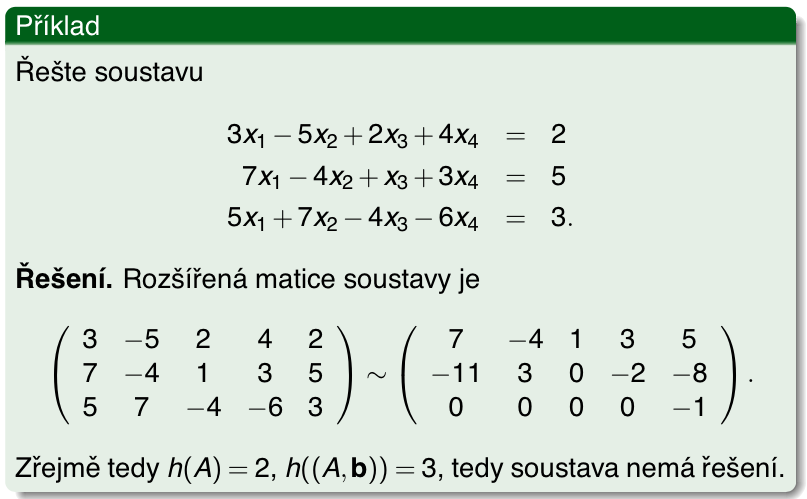
\includegraphics[scale=0.5]{img/LinSoust1}

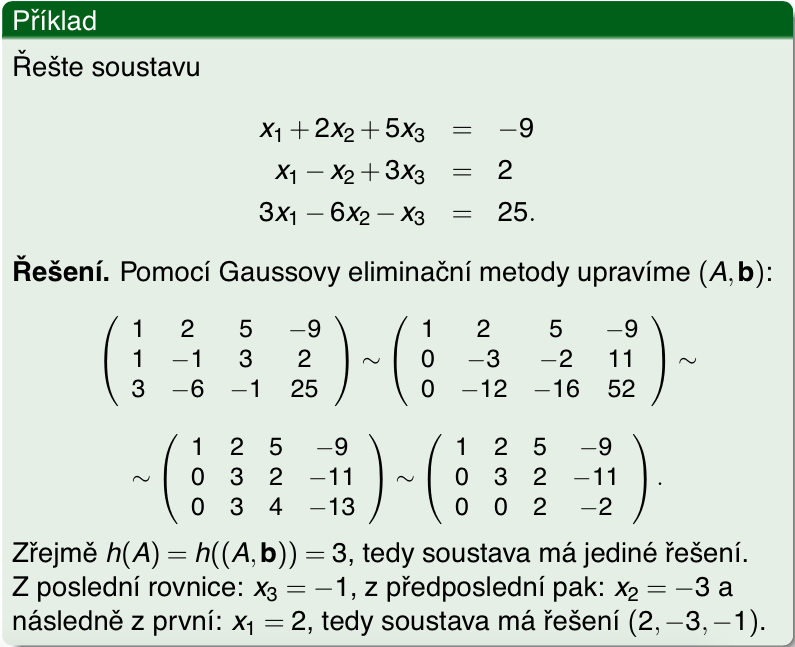
\includegraphics[scale=0.5]{img/LinSoust2}

\begin{sentence}[Cramerovo pravidlo]
	Nechť $Ax = b$ je soustava n lineárních rovnic o n neznámých $(n \geq 1)$ nad T taková, že $detA \not= 0$. Pak pro $j = 1, \dots,n$ platí $x_j = \frac{detA_j}{detA}$, kde $A_j$ je matice která vznikne z A tak, že j-tý sloupec nahradíme vektorem b.
\end{sentence}

\begin{definition}
	Fundamentálním systémem řešení homogenní soustavy lineárních rovnic rozumíme libovolnou bázi řešení této soustavy.
\end{definition}
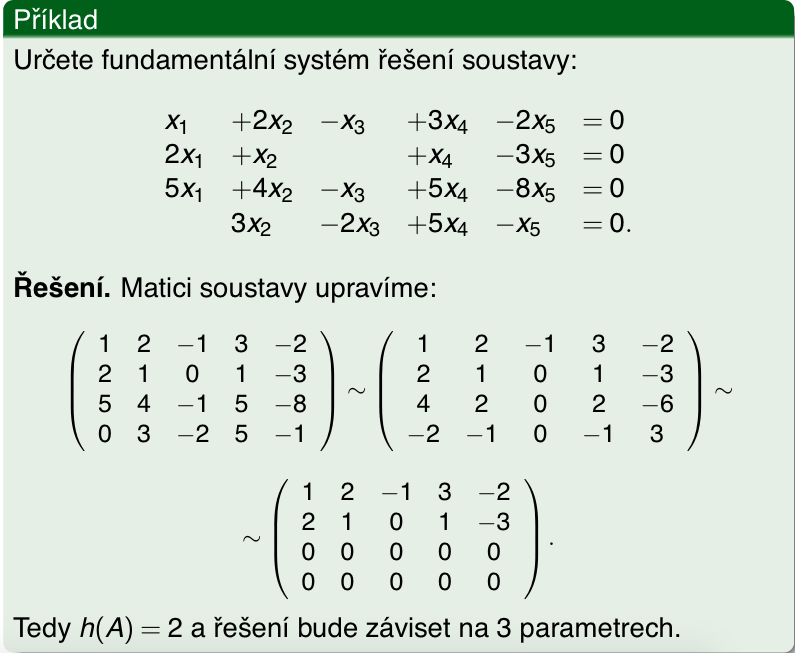
\includegraphics[scale=0.5]{img/LinSoust3}

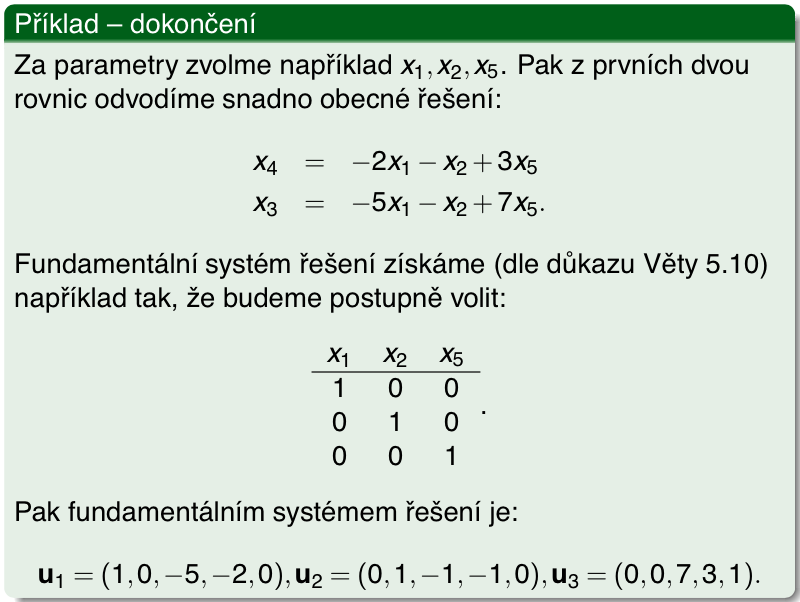
\includegraphics[scale=0.5]{img/LinSoust4}

\section{Okruh čtvercových matic}
\begin{definition}
	Matice $A \in \mathscr{M}_n(T)$ se nazývá regulární, je-li  $detA \not= 0$. Matice A je singulární, je-li $detA = 0$. 
\end{definition}

\begin{definition}
	Jestliže $A \in \mathscr{M}_n(T)$ a existuje $B \in \mathscr{M}_n(T)$, tak, že $AB = E = BA$, pak se B nazývá inverzní matice k A a značí se $B = A^{-1}$.	
\end{definition}

\begin{sentence}
	K matici $A \in \mathscr{M}_n(T)$ existuje matice inverzní právě když je A regulární
\end{sentence}

\begin{sentence}
	Množina všech regulárních čtvercových matic stupně n tvoří grupu vzhledem k násobení.
\end{sentence}

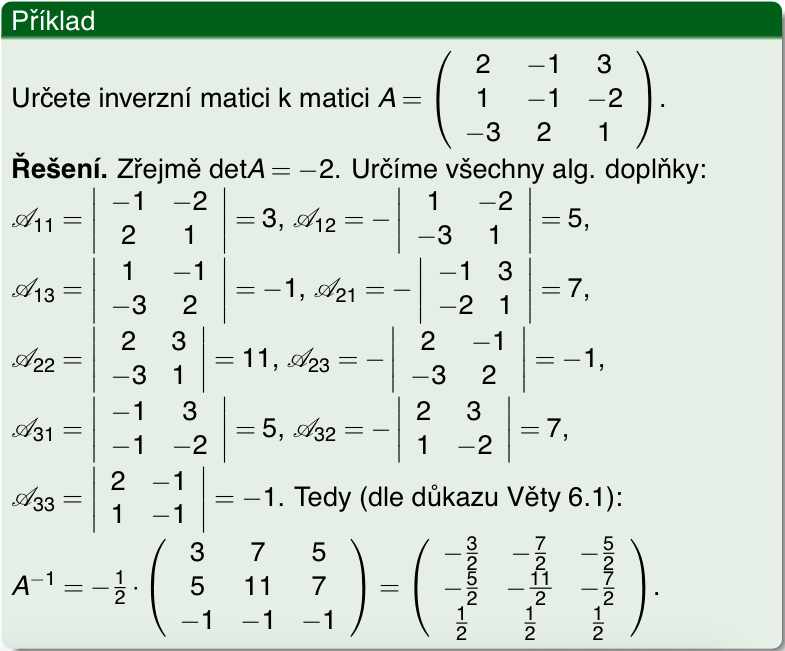
\includegraphics[scale=0.55]{img/InverzniMatice}
\newpage
\section{Svazy}

\paragraph{Polosvazem} nazýváme komutativní idempotentní pologrupu tj. takový grupoid $(G, \circ)$, kde pro každé tři prvky $a,b,c \in G$ platí tyto identity  
\begin{itemize}
	\item[a)] asociativita: $(a \circ b) \circ c = a \circ (b \circ c)$
	\item[b)] komutativita: $a \circ b = b \circ a$
	\item[c)] idempotence: $a \circ a = a$
\end{itemize}

\begin{definition}
	Nechť L je neprázdná množina, nechť $\wedge, \vee$ jsou dvě binární operace na L takové, že $(L, \wedge)$ a $(L, \vee)$ jsou polosvazy a platí tzv. zákony absorpce:
	$$(ab) \qquad a \wedge (a \vee b) = a, \qquad a \vee (a \wedge b) = a$$
	pro každé $a,b \in L$. Pak se $(L, \vee, \wedge)$ nazývá \textbf{svaz}.
\end{definition}

\paragraph{Poznámka.} Operaci $\vee$ ve svazu nazýváme \textbf{spojení}, operaci $\wedge$ nazýváme \textbf{průsek}.

\begin{definition}
	Nechť $(L, \wedge, \vee)$ je svaz, nechť $\emptyset \not= A \subseteq L$ se nazývá podsvaz svazu 
	$(L, \wedge, \vee)$, jestliže $\forall a,b \in A$ platí $a \vee b \in A,\ a \wedge b \in A$.
\end{definition}

\begin{sentence}
	Nechť L je svaz. Pak pro každé $a,b,c \in L$ platí tzv. distributivní nerovnost tj. $$a \vee (b \wedge c) \leq (a \vee b) \wedge (a \vee c), \qquad (a \wedge b) \vee (a \wedge c) \leq a \wedge (b \vee c).$$
	Pro každé $a,b,c \in L$ splňují tzv. modulární nerovnost tj. $$a \vee (b \wedge c) \leq (a \vee b) \wedge c$$
\end{sentence}

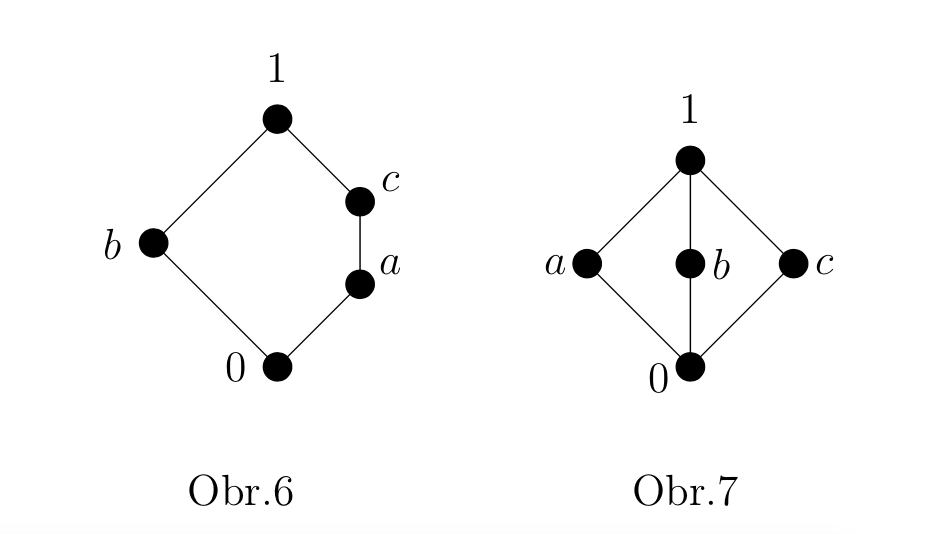
\includegraphics[scale=0.4]{img/M3aN5Svazy}

Na obrázku 6. je znázorněn svaz $N_5$ tzv. pentagon. Obrázek 7. ukazuje svaz $M_3$ jejich význam je popsán níže.

\begin{definition}
	Svaz L se nazývá distributivní, jestliže pro každé $a,b,c \in L$ platí $$(D)\qquad a \wedge (b \vee c) = (a \wedge b) \vee (a \wedge c).$$
	Svaz L se nazývá modulární, jestliže pro každé $a,b,c \in L$ splňující $a \leq c$ platí $$(M) \qquad a \vee (b \wedge c) = (a \vee b) \wedge (a \vee b).$$
\end{definition}

\begin{definition}
	Nechť $(A, \wedge, \vee)$ a $(B, \wedge, \vee)$ jsou svazy. Zobrazení $h: A \rightarrow B$ se nazývá homomorfismus, jestliže pro každé $a,b \in A$ platí: $$h(a \vee b) = h(a) \vee h(b), \qquad h(a \wedge b) = h(a) \wedge h(b)$$
\end{definition}
Bijektivní homomorfismus se nazývá \textbf{izomorfismus}.

\begin{sentence}
	Svaz L e modulární, právě když neobsahuje podsvaz izomorfní s $N_5$. Svaz je distributivní, právě když neobsahuje podsvaz izomorfní s $N_5$ nebo $M_3$ (viz obr. 6.,7.).  
\end{sentence}

\begin{definition}
	Nechť L je svaz s 0 a 1. Prvek $b \in L$ se nazývá komplement prvku $a \in L$, jestliže $$a \vee b = 1, \qquad a \wedge b = 0.$$
\end{definition}
Svaz $L$ s $0$ a $1$ se nazývá komplementární, má-li každý prvek aspoň jeden komplement.
Nechť $L$ je svaz $a,b \in L, a \leq b$ Nechť $c \in [a,b]$. Prvek $d \in [a,b]$ se nazývá relativní komplement prvku c v intervalu $[a, b]$ jestliže platí $$c \vee d = b, \qquad c \wedge d = a.$$
Svaz $L$ se nazývá relativně komplementární, má-li každá prvek $c \in [a,b]$ pro libovolné $a,b \in L,\ a \leq b$ , aspoň jeden relativní komplement v $[a,b]$.% 

% ---------------------------------------------------------------------------------------------------------
% --------------------------------------------- třetí  odstavec ---------------------------------------------
% ---------------------------------------------------------------------------------------------------------
\newpage
\textbf{Afinní prostory a podprostory, vzájemná poloha afinních podprostorů. Afinní báze, matice přechodu. Afinní
zobrazení a jejich matice. Eukleidovské afinní prostory. Projektivní prostory a homogenní souřadnice. Aplikace
v počítačové grafice.}
\section{Afinní prostory (AP)}
Řekněme, že na neprázdné množině $A$ je dána \textit{struktura afiního prostoru} (stručněji afinní struktura), je-li dán vektorový prostor $U$ a zobrazení $Add_A : A \times U \rightarrow A$ takové, že 
\begin{enumerate}
	\item pro všechna $a \in A,\ u,v, \in U$ $$Add_A(Add_A(a,u), v) = Add_A(a, u + v)$$
	\item pro všechna $a,b \in A$ existuje právě jedno $u \in U$ tak, že $$Add_A(a,u) = b$$
\end{enumerate}

Množina $A$ se strukturou afinního prostoru se nazývá afinní prostor, její prvky se nazývají body, Vektorový prostor $U$ se nazývá zaměřením afinního prostoru $A$.

Zobrazení $Add_A$ se nazývá sčítání bodů a vektorů. Pro libovolné $a \in A$ a $u \in U$ se bod $Add_A(a, u)$ označuje $a + u$ a nazývá se součet bodu $a$ a vektoru $u$.

Jelikož podle bodu 1. definice platí $(a + u) + v = a + (u + v)$, můžeme při sčítání dvou vektorů k bodu vynechat závorky a psát pouze $(a + u + v)$.

Vektor $u$ z 2. bodu definice afinního prostoru se označuje $b - a$. Vzhledem k podmínce bodu 2. tento vektor existuje pro libovolné $a$ a $b$ a to právě jeden. Přiřazením $(a,b) \mapsto b - a$ je tedy jednoznačně určené zobrazení z $A \times A$ do $U$. Vektoru $b - a$ se říká rozdíl bodů $b$ a $a$.

\begin{center}
	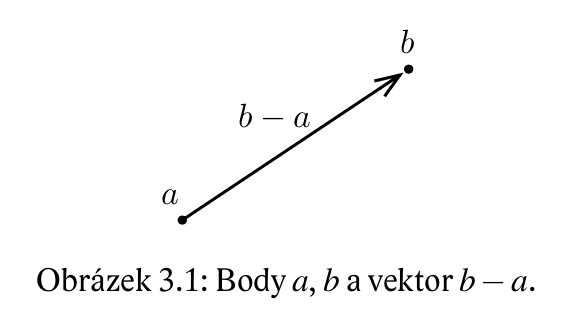
\includegraphics[scale=0.5]{img/Vektor_b-a}
	
	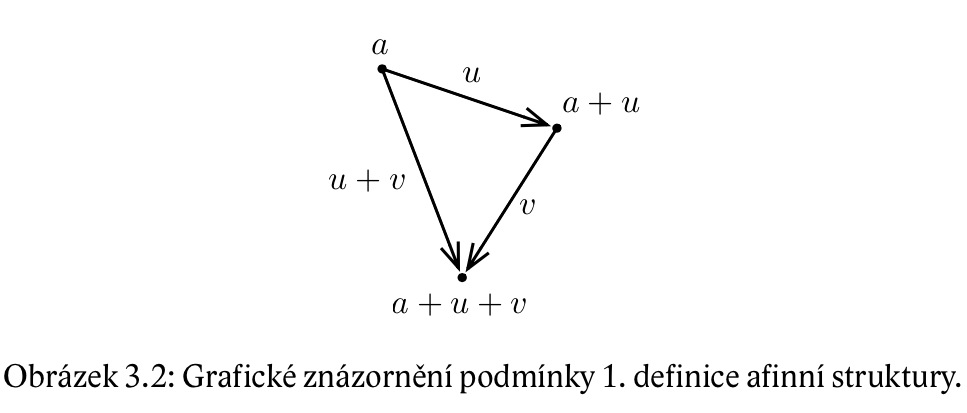
\includegraphics[scale=0.4]{img/definiceAfProst}
\end{center}

Je-li vektorový prostor $U$ konečné dimenze $\Rightarrow$ afinní prostor je také konečné dimenze. Dimenzí AP $A$ nazýváme dimenzi vektorového prostoru $V$. Afinní prostor dimenze 1 se nazývá afinní přímka, afinní prostor dimenze 2 afinní rovina.

\subsection{Afinní kombinace a afinní obal}
\begin{center}
	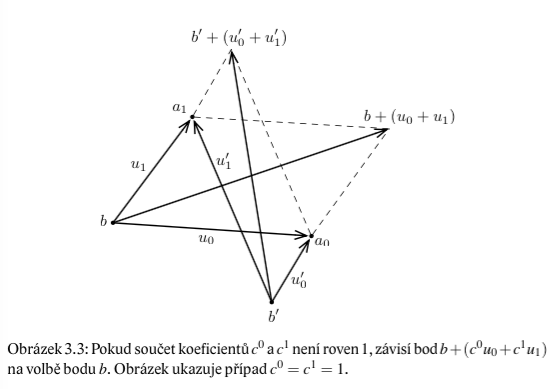
\includegraphics[scale=0.7]{img/AfinniObal}
\end{center}
Začněme pozorováním. Na obrázku 3.3 vidíme body $a_0,a_1,b$ afinního prostoru $A$. Dvojice bodů $a_0,b$ a $a_1$ definují vektory $u_0 = a_0 - b$ a $u_1 = a_1 - b$, které jsou na obrázku rovněž znázorněny. Lineární kombinace $c^0u_0 + c^1u_1$ těchto vektorů pak definujeme bod $b + (c^0u_0 + c^1u_1)$ (na obrázku je znázorněn připad $c^0 = c^1 = 1$). POkud místo bidu $b$ vybereme nějaký jiný bod $b'$, pak se výsledný bod získaný stejným způsobem, bude od původního lišit: $$b + (c^0u_0 + c^1u_1) \not= b' + (c^0u'_0 + c^1u'_1),$$
což e patrné i z obrázku

Situace se ovšem mění, pokud $c^0 + c^1 =  1$. To můžeme odhadnout už na obrázku 3.3 když se podíváme na průsečík šipek znázorňující vektory $u_0 + u_1$ a $u'_0 + u'_1$. Na obrázku 3.4 jsou zobrazeny případy $c^0 =  c^1 = \frac{1}{2}$ a $c^0 = 1$ a $c^1 = -1$. Zřejmě pokud $c^0 + c^1 = 1$, pak $b + (c^0u_0 + c^1u_1) = b' + (c^0u'_0 + c^1u'_1)$. Následující věta naši domněnku potvrzuje pro libovolný počet bodů.

\begin{sentence}
	Mějme body $a_0,a_1, \dots, a_m$ afinního prostoru A. Pro libovolné dva body $b,b' \in A$ a čísla $c^0, c^1, \dots, c^m$ taková, že  $c^0 + c^1 + \dots + c^m = 1$ platí
	$$b + c^0(a_0 - b) + c^1(a_1 - b) + \dots + c^m(a_m - b) = b' + c^0(a_0 - b') + c^1(a_1 - b') + \dots + c^m(a_m - b')$$
\end{sentence}

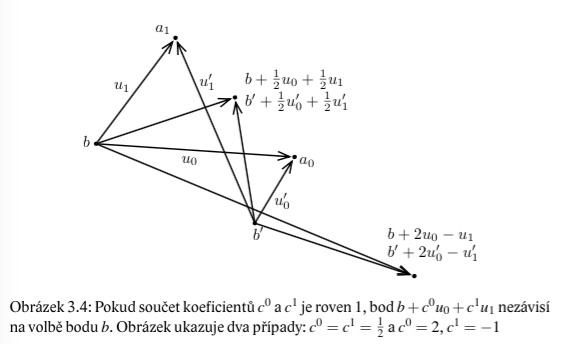
\includegraphics[scale=0.7]{img/AfinniObal2}

Každou afinní kombinaci více než dvou bodů lze vyjádřit pomocí afinních kombinací dvojic bodů. Ukážeme se to na příkladě afinní kombinace $c^0a_0 + c^1a_1 + c^2a_2$. Pokud je $c^0 + c^1 \not= 0$, platí: $$c^0a_0 + c^1a_1 + c^2a_2  = (c^0 + c^1) \left( \frac{c^0}{c^0 + c^1}a_0 + \frac{c^1}{c^0 + c^1}a_1 \right) + c^2a_2,$$ přičemž $\frac{c^0}{c^0 + c^1} + \frac{c^1}{c^0 + c^1} = 1$, takže uvnitř velké závorky je opravdu afinní kombinace dvou bodů, stejně jako je afinní kombinací dvou bodů i celý výraz, protože $(c^0 + c^1) + ^2 = 1$. 

\paragraph{Afinní obal} množiny $K$ je množina značící se $Aff(K)$ definovanou následovně: $$Aff(K) = \{ c^0a_0 + c^1a_1 \ | \ a_0,a_1 \in K, c^0 + c^1 = 1\}$$

\begin{sentence}
	Pro libovolnou neprázdnou množinu $K \subseteq A$ platí $Aff(Aff(K)) = Aff(K)$.
\end{sentence}

\subsection{Vektorové kombinace}
Pokud $c^0 + c^1 + \dots + c^m = 0$, pak vektor $$c^0(a_0 - b) + c^1(a_1 - b) + \dots + c^k(a_k - b)$$nezávisí na volbě bodu $b$. Body $a_0,a_1 \dots, a_k$ spolu s koeficienty $c^0,c^1, \dots, c^k$ tak jednoznačně definují vektor. který se nazývá vektorová kombinace bodů $a_0,a_1 \dots, a_k$. tento vektor se značí stejně jako kombinace afinní: $$c^0a_0 + c^1a_1 + \dots + c^ka_k.$$

Pro neprázdnou množinu $K \subseteq A$ označujeme symbolem $Vec(K)$ množinu všech vektorových kombinací prvků množiny $K$. Platí $$Vec(K) = \{ c^0a_0 + \dots + c^ka_k \ | \ k \geq 1, a_0,\dots a_k \in K, c^0 + \dots + c^k = 0\}$$

\begin{sentence}
	Vec(K) je vektorový podprostor zaměření afinního prostoru.
\end{sentence}

\begin{sentence}
	Vec(Aff(K)) = Vec(K) 
\end{sentence}

\subsection{Afinní podprostory}
Neprázdná podmnožina $B$ afinního prostoru $A$ se zaměřením $U$ se nazývá afinní podprostor afinního prostoru $A$, jestliže $Aff(B) = B$

\begin{sentence}
	Neprázdná podmnožina B afinního prostoru A se zaměřením U je jeho afinním podprostorem, právě když existuje vektorový prostor $V \subseteq U$ takový, že jsou splněny následující podmínky: 
	\begin{enumerate}
		\item Pro každé $a \in B, \ u \in V$ platí $a + u \in B$
		\item Pro každé $a,b \in B$ platí $b - a \in V$
	\end{enumerate}
	Platí V = Vec(B).
\end{sentence}

\subsubsection{Vzájemná poloha afinních podprostorů}
Mějme dva afinní podprostory $B_1$ a $B_2$ se zaměřeními $V_1,\ V_2$ afinního prostoru $A$ se zaměřením $U$. O afinních podprostorech $B_1,B_2$ řekneme, že jsou 
\begin{description}
	\item[rovnoběžné], pokud platí $V_1 \subseteq V_2$ nebo $V_2 \subseteq V_1$,
	\item[různoběžné], pokud nejsou rovnoběžné a pokud $B_1 \subseteq B_2 \not= \emptyset$.
	\item[mimoběžné] ve všech ostatních případech. 
\end{description}

\begin{sentence}
	Předpokládejme, že afinní podprostory $B_1,B_2$ jsou rovnoběžné a, že $V_1 \subseteq V_2$. Následující 3 podmínky jsou ekvivalentní:
	\begin{enumerate}
		\item Existuje bod $b_0 \in B_1 \cap B_2$.
		\item Pro každé dva body $b_1 \in B_1$ a $b_2 \in B_2$ platí $b_2 - b_1 \in V_2$.
		\item Existují body $b_1 \in B_1$ a $b_2 \in B_2$ takové, že $b_2 - b_1 \in V_2$. 
	\end{enumerate}
\end{sentence}

\begin{sentence}
	Předpokládejme, že afinní podprostory $B_1,B_2$ nejsou rovnoběžné a, že $V_1 \subseteq V_2$. Následující 3 podmínky jsou ekvivalentní:
	\begin{enumerate}
		\item $B_1$ a $B_2$ jsou různoběžné.
		\item Pro každé dva body $b_1 \in B_1$ a $b_2 \in B_2$ platí $b_2 - b_1 \in V_1 \vee V_2$.
		\item Existují body  $b_1 \in B_1$ a $b_2 \in B_2$ takové, že $b_2 - b_1 \in V_1 \vee V_2$. 
	\end{enumerate}
\end{sentence}
\paragraph{Poznámka.} Symbolem \uv{$\vee$} označujeme operaci spojení vektorových prostorů.


\subsection{Afinní báze}
Mějme afinní prostor $A$ dimenze $m$ se zaměřením $U$. pro bod $a_0 \in A$ a bázi $\alpha = (u_1, \dots, u_m)$ vektorového prostoru $U$ nazýváme dvojici $\varphi '(\alpha, a_0)$ afinní bázi afinního prostoru $A$. Bod $a_0$ nazýváme počátkem báze $\varphi$. Afinní bázi $\varphi$ zapisujeme jako $(m + 1)$-tici $(u_1, \dots, u_m,a_0)$. Pro libovolný bod $a \in A$ nazýváme afinními souřadnicemi (souřadnicovým vyjádřením) bodu a vzhledem k afinní bázi $\varphi = (\alpha, a_0)\ (m + 1)$-tici
\begin{displaymath}
	\alpha_\varphi = \left[ \begin{array}{c}
						(a - a_0)^1_\alpha \\
						(a - a_0)^2_\alpha \\
						\vdots \\
						(a - a_0)^m_\alpha \\
						1 
					    \end{array} \right]
\end{displaymath}

\subsubsection{Matice přechodu}
Mějme dvě afinní báze $\varphi = (\alpha, a_0), \ \overline{\varphi} = (\overline{\alpha}, \overline{a_0})$ afinního prostoru $A$ dimenze $m$ se zaměřením $U$.  Problém jak najít souřadnicové vyjádření bodu $a \in A$ vzhledem k bázi $\overline{\varphi}$ známe-li souřadnicové vyjádření tohoto bodu vzhledem k bázi $\varphi$. K výpočtu potřebujeme znát souřadnice bodu $a$ v afinní bázi $\varphi$, matici přechodu od (vektorové) báze $\alpha$ k $\overline{\alpha}$ a souřadnice počátku $a_0$ vzhledem k afinní bázi $\overline{\varphi}$. Matici $M_{\varphi,\overline{\varphi}}$ přechodu od báze $\varphi$ k bázi $\overline{\varphi}$ definujeme následovně:
\begin{center}
	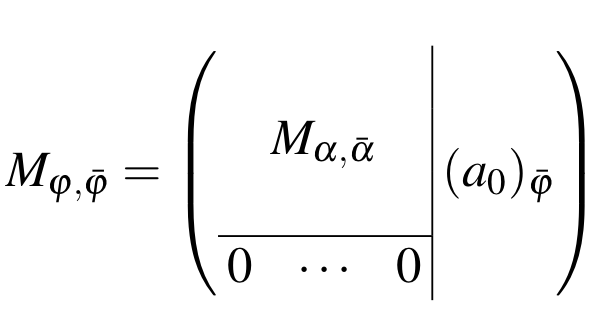
\includegraphics[scale=0.4]{img/MaticePrechodu}
\end{center}

\paragraph{Použití.} Pří kreslení v OpenGL se používají dvě základní afinní báze: Báze modelu (Model Coordinate System) a Báze pozorovatele (View Coordinate System). Báze modelu je báze, vzhledem k níž uvádíme souřadnice vykreslovaných objektů. Báze pozorovatele je spojena s kamerou tak, že první vektor její vektorové báze směřuje doprava, druhý nahoru a třetí dozadu.

\begin{center}
	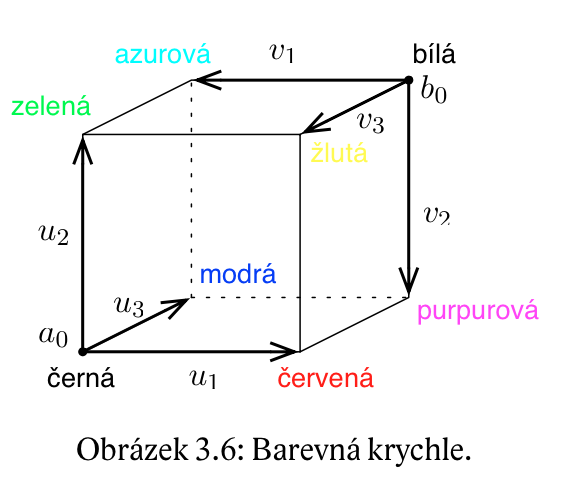
\includegraphics[scale=0.4]{img/KrychleBarevnychModelu}
\end{center}


\paragraph{Použití.} na obrázku 3.6 vidíme základních osm barev (bílou, černou, červenou, zelenou, modrou, žlutou, azurovou a purpurovou) uspořádaných do vrcholů tzv. barevné krychle. Tuto krychli si můžeme představit jako podmnožinu trojrozměrného afinního prostoru; body mimo ni pro nás ovšem nemají význam. Na obrázku jsou zakresleny dvě základní afinní báze, které se používají k vyjádření barev: $\varphi_{RGB} = (u_1,u_2,u_3,a_0)$ a  $\varphi_{CMYK} = (v_1,v_2,v_3,b_0)$. Matice přechodu vypadá následovně:
\begin{center}
	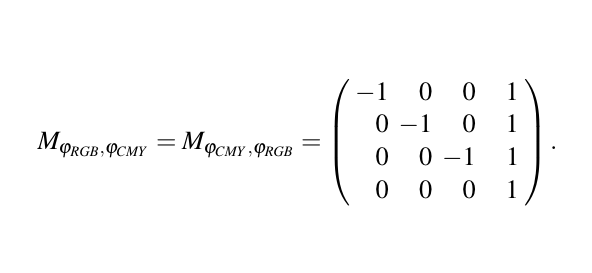
\includegraphics[scale=0.6]{img/MaticePrechoduRGB_CMYK}
\end{center}

\subsection{Afinní zobrazení}
Afinní zobrazení jsou zobrazení, která jsou popsatelná v rámci teorie afinních prostorů. Mezi afinní zobrazení patří mnohá zobrazení, která se používají v počítačové grafice: posunutí, otočení, změna měřítka, atd.

\begin{definition}
	Zobrazení $f : A \rightarrow B$ afinních prostorů $A$ a $B$ se nazývá afinní, jestliže pro libovolné dva body $a_1,a_2 \in A$ a jejich afinní kombinaci $c^1a_1 + c^2a_2$ platí $$f(c^1a_1 + c^2a_2) = c^1f(a_1) + c^2f(a_2).$$
\end{definition}

\begin{sentence}
	Pro lib. bod $b_0 \in B$ je zobrazení $f : A \rightarrow B$, definované předpisem $f(a) = b_0$ (tj. konstantní zobrazení), afinní.
\end{sentence}

\begin{sentence}
	Identické zobrazení (identita) na množině X je zobrazení $Id_X$ takové, že $Id_X(x) = x$ pro každé $x \in X$. Identita na afinním prostoru A je afinní zobrazení.
\end{sentence}

\begin{sentence}
	Zobecnění předchozí věty: je-li $Y \subseteq X$, pak kanonické vložení podmnožiny Y do X je zobrazení $i_Y : Y \rightarrow X$, definované předpisem $i_Y(y) = y$. Je-li $B \subseteq A$ afinní podprostor afinního prostoru A, pak kanonické vložení $i_B : B \rightarrow A$ je afinní zobrazení.  
\end{sentence}

\begin{sentence}
	Zobrazení $f_0 : U \rightarrow V$ definované předpisem (věta 45) se nazývá zobrazení podřízene afinnímu zobrazení f.
\end{sentence}
\begin{sentence}
	Kompozice dvou afinních zobrazení je afinní zobrazení.
\end{sentence}

\begin{sentence}
	Afinní zobrazení $f : A \rightarrow A$ se nazývá afinní transformace afinního prostoru A.	
\end{sentence}

\begin{sentence}
	Příkladem afinní transformace afinního prostoru A je posunutí o vektor $u_0 \in U$, což je zobrazení $tr_{u_0} : A \rightarrow A$ (tr jako translace) definované předpisem $$r_{u_0}(a) = a + u_0.$$
\end{sentence}

\begin{center}
	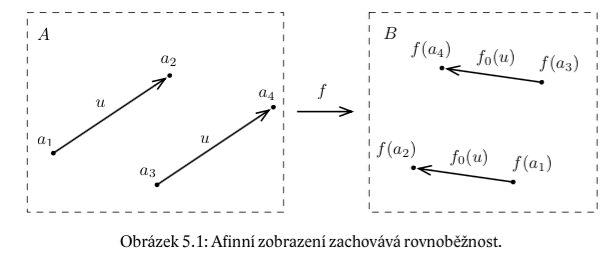
\includegraphics[scale=0.7]{img/AfinniZobrazeni}
\end{center}

\begin{sentence}
	Středová souměrnost se středem $a_0 \in A$ je zobrazení $f : A \rightarrow A$ definované předpisem $$f(a) = 2a_0 - a$$ 
\end{sentence}
\begin{sentence}
	Zobrazení $f : A \rightarrow A$ se nazývá stejnolehlost pokud platí $$f(a) = (1 - c)a_0 + ca.$$
\end{sentence}

\begin{center}
	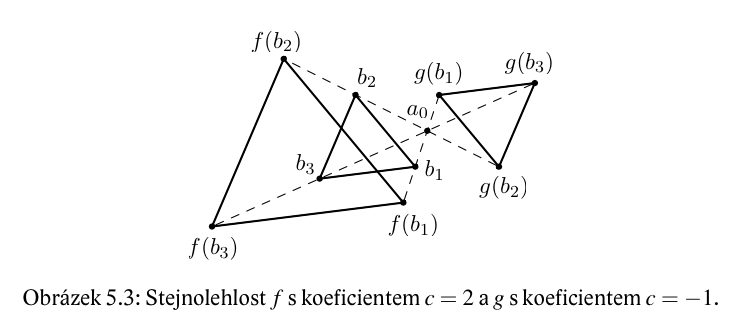
\includegraphics[scale=0.6]{img/Stejnolehlost}
\end{center}


\subsubsection{Matice affiního zobrazení}
Mějme afinní bázi $\varphi = (\alpha, a_0),\ \alpha = (u_1, \dots, u_m)$ afinního prostoru $A$ se zaměřením $U$ a afinní bázi $\psi = (\beta, b_0),\ \beta = (v_1, \dots, v_n)$ afinního prostoru $B$ se zaměřením $V$. Dále mějme afinní zobrazení $f : A \rightarrow B$ s podřízeným lineárním zobrazením $f_0 : U \rightarrow V$. Naším cílem je najít způsob, jak ze souřadnicového vyjádření $a_\varphi$ bodu $a \in A$ vzhledem k bázi $\varphi$ vypočítat souřadnicové vyjádření $f(a)_\psi$ jeho obrazu $f(a)$ při zobrazení f vzhledem k bázi $\psi$.

\begin{center}
	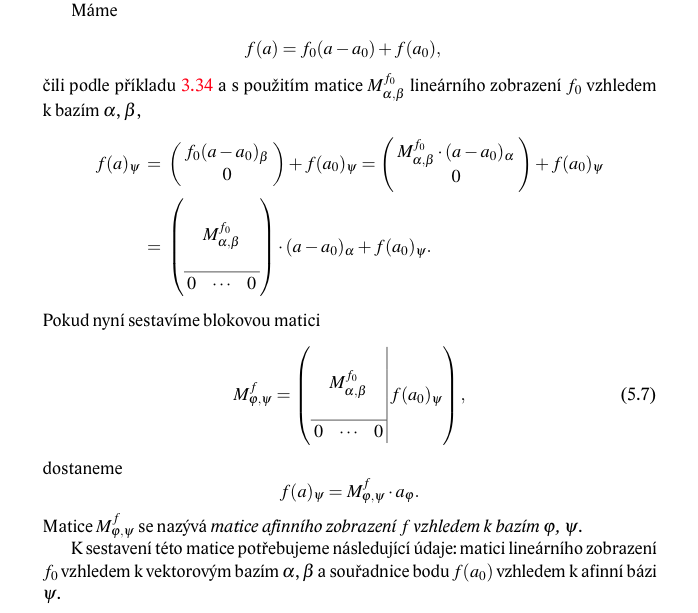
\includegraphics[scale=0.6]{img/MaticeAfinnihoZobrazeni}
\end{center}

\section{Eukleidovské prostory}
\begin{center}
	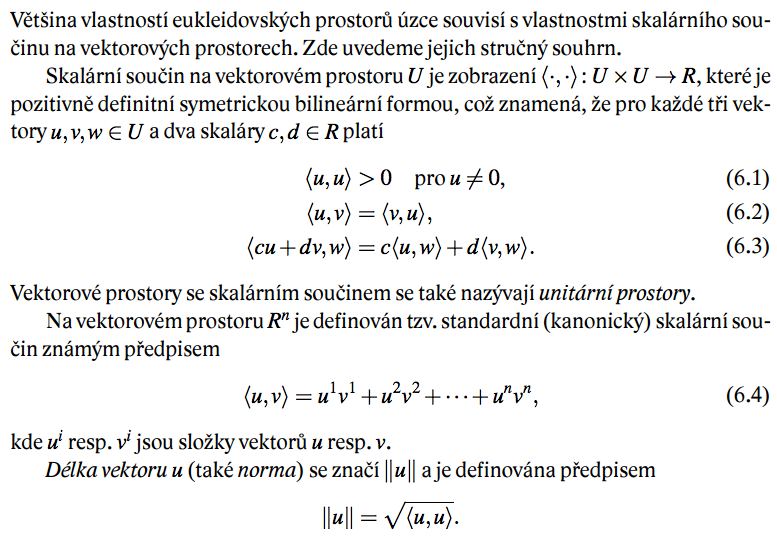
\includegraphics[scale=0.5]{img/EukleidovskeProstory1}
\end{center}
\begin{center}
	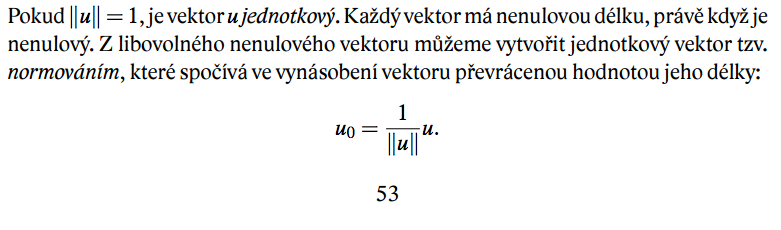
\includegraphics[scale=0.5]{img/EukleidovskeProstory2}
\end{center}
\begin{center}
	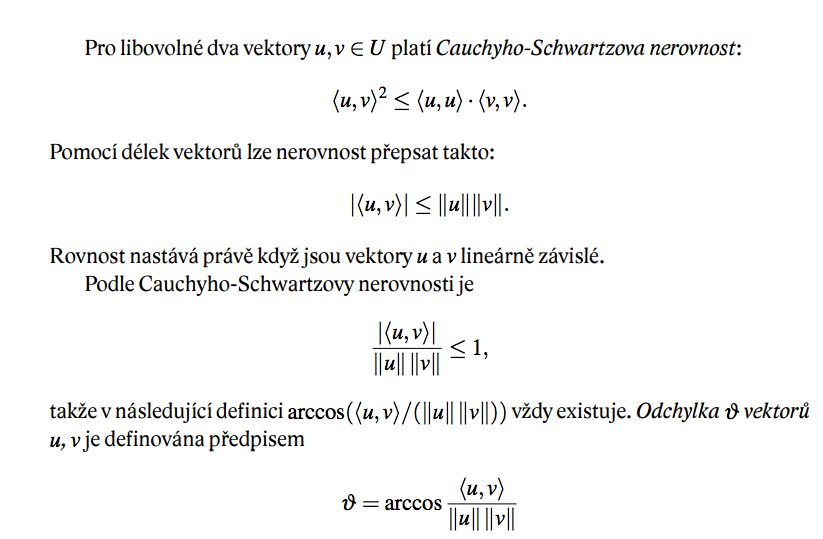
\includegraphics[scale=0.5]{img/EukleidovskeProstory3}
\end{center}
\begin{center}
	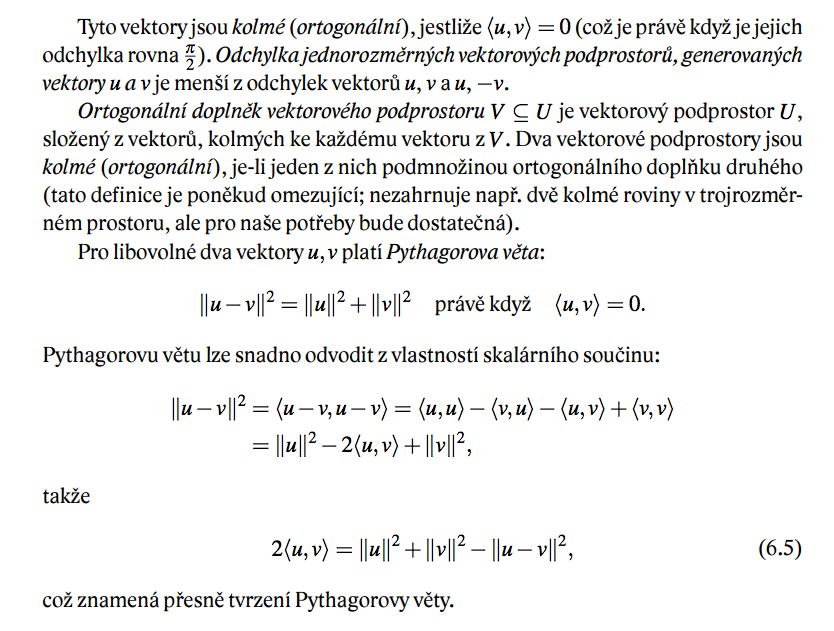
\includegraphics[scale=0.5]{img/EukleidovskeProstory4}
\end{center}

\section{Projektivní prostory}
\begin{center}
	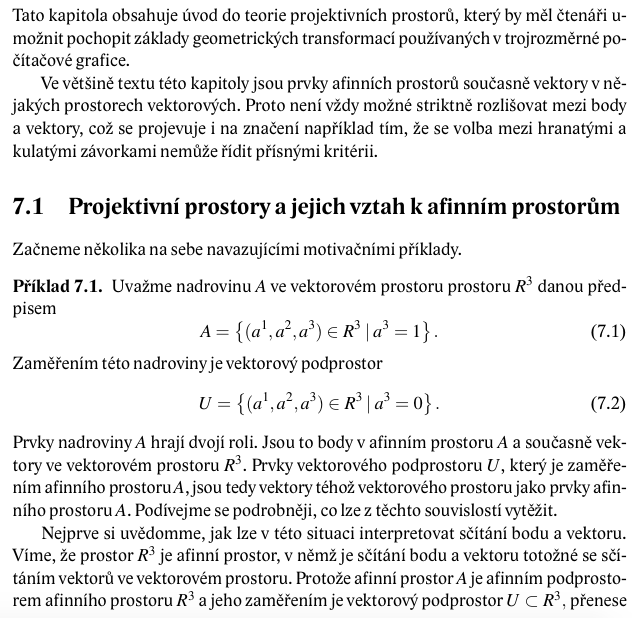
\includegraphics[scale=0.6]{img/ProjektivniProstor1}
\end{center}
\begin{center}
	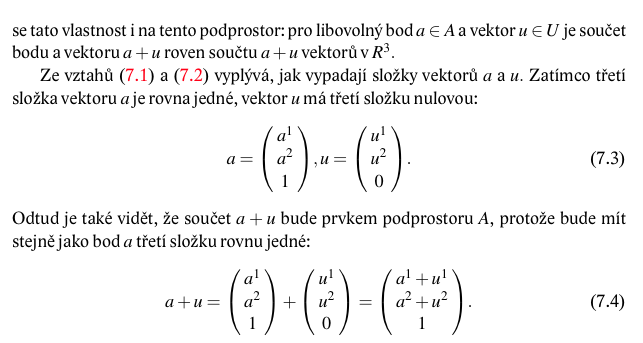
\includegraphics[scale=0.6]{img/ProjektivniProstor2}
\end{center}

\subsection{Projektivní zobrazení}
\begin{center}
	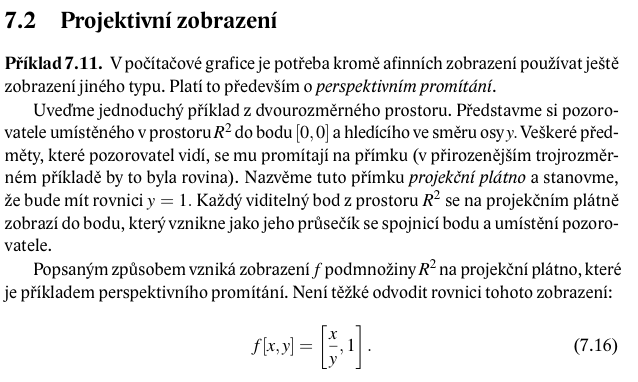
\includegraphics[scale=0.6]{img/ProjektivniZobrazeni1}
\end{center}
\begin{center}
	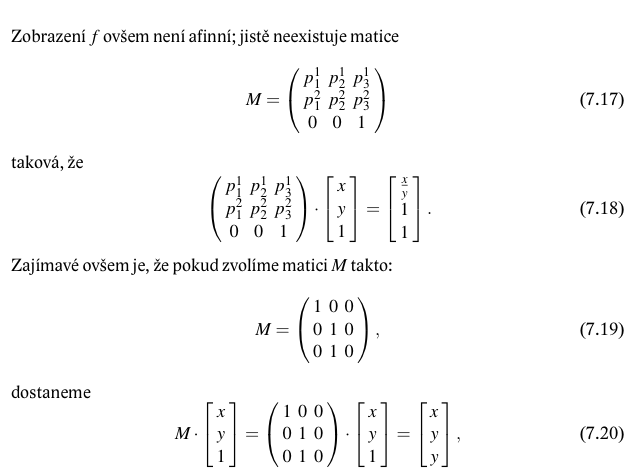
\includegraphics[scale=0.6]{img/ProjektivniZobrazeni2}
\end{center}
\newpage
% ---------------------------------------------------------------------------------------------------------
% --------------------------------------------- čtvrty  odstavec ---------------------------------------------
% ---------------------------------------------------------------------------------------------------------
\textbf{Posloupnosti a jejich limity. Funkce jedné reálné proměnné a jejich vlastnosti. Limita a spojitost funkce. Derivace funkce, geometrický význam. Základní věty diferenciálního počtu a jejich aplikace. Vyšetřování průběhu funkce. Neurčitý integrál, určitý Riemannův integrál. Číselné řady, konvergence a součty, kriteria konvergence}

\section{Funkcia jednej reálnej premennej a jej vlastnosti}
\textbf{Funkciou reálnej premennej} rozumieme lubovolné zobrazenie $f : X \rightarrow \mathds{R}$, kde $X \subseteq \mathds{R}$. ($f: X \subseteq \mathds{R} \rightarrow \mathds{R}$)

\subsection{Vlastnosti}
\begin{definition}
	Funckia $f: X \subseteq \mathds{R} \rightarrow \mathds{R}$ sa nazýva \textbf{ohraničená} (zhora, zdola alebo len ohraničená) na množine $X'\subseteq X$, ak je taká množina $f(X')\subseteq \mathds{R}$.
\end{definition}

\begin{definition}
	\textbf{Maximom} funkcie $f: X \subseteq \mathds{R} \rightarrow \mathds{R}$ na množine $X'\subseteq X$ nazývame číslo \textbf{max}$f(X')$ (značenie: $max_{x\in X'}f(X)$). Povieme že funkcia $f$ tejto hodnoty nabýva v bode $x\in X'$, ak $f(x)=max f(X')$.
\end{definition}

\begin{definition}
	\textbf{Minimom} funkcie $f: X \subseteq \mathds{R} \rightarrow \mathds{R}$ na množine $X'\subseteq X$ nazývame číslo \textbf{min}$f(X')$ (značenie: $min_{x\in X'}f(X)$). Povieme že funkcia $f$ tejto hodnoty nabýva v bode $x\in X'$, ak $f(x)=min f(X')$.
\end{definition}

\paragraph{} 
O maxime (poprípade minime) funkcie $f$ na množine $X'\subseteq X$ je \textbf{ostré}, ak existuje práve jeden bod tejto množiny, v ktorej funkcia $f$ maxima (poprípade minima) nabýva. Ak je takých bodov viac, hovoríme že maximum (poprípade minimum) je \textbf{neostré}. Maximum a minimum sa súhrne nezývajú \textbf{extrémy}. Bod, v ktorom funkcia nabýva maxima (poprípade minima) na danej množine vždy existuje. To ale nemusí platiť o supréme a infime (definície nasledujú). Majme množiny $B \subseteq A$ (na množine $A$ je zavedené usporiadanie) pričom platí $A, B \subseteq \mathds{R}$, potom \textbf{hornou závorou} množiny $B$ rozumieme taký prvok $a\in A$, že $\forall b\subseteq B$ platí, $b\leq a$. Analogicky \textbf{dolnou závorou} množiny $B$ rozumieme taký prvok $a\in A$, že $\forall b\subseteq B$ platí, $a\leq b$. \vspace{0.5cm}

\begin{definition}
	\textbf{Supremom funkcie} $f: X \subseteq \mathds{R} \rightarrow \mathds{R}$ na množine $X'\subseteq X$ nazývame číslo \textbf{sup}$f(X')$ (značenie: $sup_{x\in X'}f(X)$). (Sedlácky povedané, supremum je najmenší prvok z množiny všetkých horných závor oboru hodnot funkcie na danom intervale.)
\end{definition}

\begin{definition}
	\textbf{Infimom funkcie} $f: X \subseteq \mathds{R} \rightarrow \mathds{R}$ na množine $X'\subseteq X$ nazývame číslo \textbf{inf}$f(X')$ (značenie: $inf_{x\in X'}f(X)$). (Sedlácky povedané, infimum je najvačší prvok z množiny všetkých dolných závor oboru hodnot funkcie na danom intervale.)
\end{definition}

\begin{definition}
	Povieme že funkcia $f: X \subseteq \mathds{R} \rightarrow \mathds{R}$ je na množine $X'\subseteq X$ \textbf{rastúca (nerastúca, klesajúca, neklesajúca)}, ak pre každé 2 body $x, y \in X', x<y$, platí $f(x)<f(y) (f(x) \geq f(y), f(x)>f(y), f(x)\leq f(y))$. Ak je funkcia $f$ rastúca (nerastúca, klesajúca, neklesajúca) na celej množine $X$, nazýva sa proste rastúca (nerastúca, klesajúca, neklesajúca). Súhrne sa taká funkcia nazýva \textbf{monotónnou}.
\end{definition}

\begin{definition}
	Povieme že funkcia $f: X \subseteq \mathds{R} \rightarrow \mathds{R}$ je \textbf{konvexná} na intervale $I\subseteq X$, ak pre každé tri body $x, y, z\in I, x<y<z$, platí $f(x)(z-y)+f(y)(x-z)+f(z)(y-x)\geq 0$.
\end{definition}

\begin{definition}
	Povieme že funkcia $f: X \subseteq \mathds{R} \rightarrow \mathds{R}$ je \textbf{konkávna} na intervale $I\subseteq X$, ak pre každé tri body $x, y, z\in I, x<y<z$, platí $f(x)(z-y)+f(y)(x-z)+f(z)(y-x)\leq 0$.
\end{definition}

\begin{figure}[ht]
	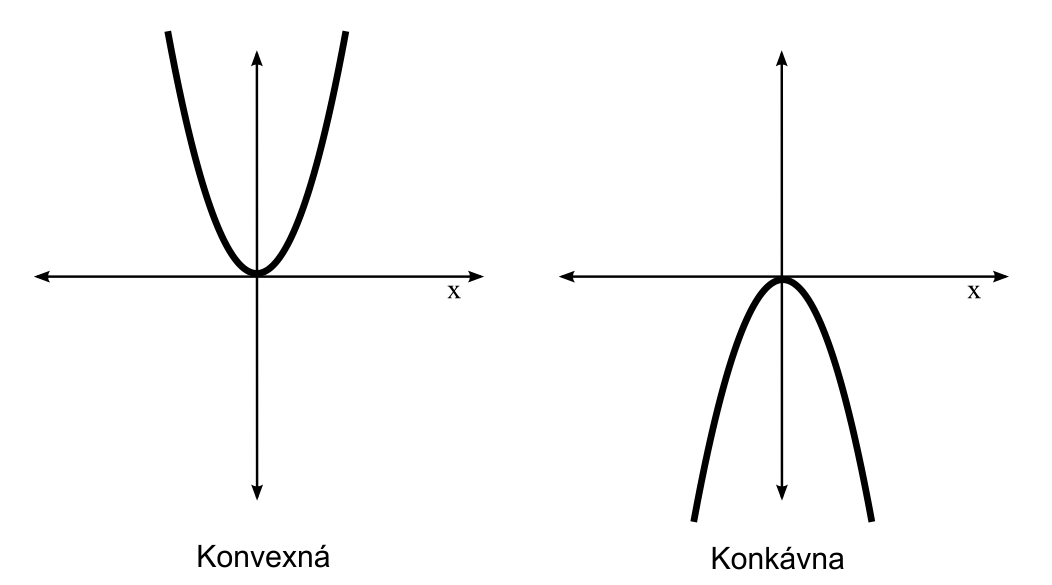
\includegraphics[scale=0.53]{img/konvexna_konkavna}
	\caption{\textbf{Hint:} Do konkávnej kávu nenaleješ!}
\end{figure}

\begin{definition}
	Funkcia $f: X \subseteq \mathds{R} \rightarrow \mathds{R}$ sa nazýva \textbf{sudá (lichá)}, ak pre každý bod $x\in X$ platí $-x\in X$ a $f(-x) = f(x) (f(-x) = -f(x))$ (Príklad lichej: $f(x)=x^{3}$).
\end{definition}

\begin{definition}
	Funkcia $f: X \subseteq \mathds{R} \rightarrow \mathds{R}$ sa nazýva \textbf{periodická}, ak existuje číslo $p>0$ také, že $x\in X$, práve vtedy keď $x+p \in X$ a ak $x\in X$, potom $f(x+p)=f(x)$. Číslo $p$ na nazýva \textbf{perióda funkcie} $f$. (Príklad: $f(x)=sin(x)$ s periódou $p=2\pi$) 
\end{definition}

\begin{definition}
	Funkcia $f: X \subseteq \mathds{R} \rightarrow \mathds{R}$ taká, že jej obor hodnot je jednoprvková množina, sa nazýva \textbf{konštantná funkcia}
\end{definition}

\begin{definition}
	Funkcia $f: \mathds{R} \rightarrow \mathds{R}$ sa nazýva \textbf{afinná}, ak existujú čísla $p,q \in \mathds{R}$ také, že pre každé $x \in \mathds{R}$ platí $f(x)=px+q$. Množina $Y\subseteq\mathds{R}^{2}$ sa nazýva \textbf{priamka}, ak existujú čísla $a, b \in \mathds{R}$ ktoré niesú súčastne rovné 0, také, že $Y=\{(x, y)\in\mathds{R}^{2}|ax+by=0\}$. (Veta: Funkcia $f: \mathds{R} \rightarrow \mathds{R}$ je afinná, práve vtedy keď je jej grafom priamka. Dokaz si podľa \\doc. Krupku urobíme s radosťou sami.)
\end{definition}

\subsection{Operácie s funkciami}
\paragraph{}
Majme funkcie $f, g: X\subseteq\mathds{R}\rightarrow\mathds{R}$. Funkciu $(f+g):X\rightarrow\mathds{R}$, definovanú pre každé $x\in X$ prepisom $(f + g)(x)=f(x)+g(x)$ nazveme \textbf{súčtom fumkcií} $f$ a $g$. \textbf{Súčinom týchto funkcií} nazývame funkciu $(f\cdot g):X\rightarrow\mathds{R}$, definovanú pre každé $x\in X$ predpisom $(f \cdot g)(x)=f(x)\cdot g(x)$


\subsection{Príklady špeciálnych funkcií}
\paragraph{}
\textbf{Absolútnou hodnotou} reálneho čísla $x$ nazývame číslo $|x|$, ktoré je rovné $x$, ak je $x\geq 0$ a rovné $-x$, ak je $x<0$. Tým dostávame funkciu $[\cdot]:\mathds{R}\rightarrow\mathds{R}$ \\ \vspace{-1cm}
\paragraph{}
\textbf{Celou časťou} reálneho čísla $x$ nazývame najvačšie celé číslo, ktoré je menšie alebo rovné $x$. Dostávame funkciu $[x]:\mathds{R}\rightarrow\mathds{R}$ \\ \vspace{-1cm}
\paragraph{}
Pre reálne číslo $x$ kladieme $\chi(x)=0$, ak $x\in \mathds{I}$, a $\chi(x)=1$, ak $x\in \mathds{Q}$. Dostávame \textbf{Dirichletovu funkciu} $\chi:\mathds{R}\rightarrow\mathds{R}$

\begin{figure}[ht]
	\begin{center}
		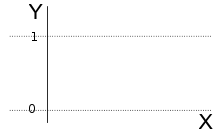
\includegraphics{img/dirichletova_funkce}
	\end{center}
	\caption{Dirichletova funkcia}
\end{figure}

\section{Limita a spojitosť funkcie}

\subsection{Opakovanie základov topológie}
\textcolor{red}{Z topológie sú tu len pojmy potrebné na definíciu spojitosti funkcie.}
\begin{definition}
	\textbf{Topologický priestor:} Na množine $X$ je zadaná topólogia, ak je určrný systém $\tau$(Tau) podmnožín $X$ splňujúci podmienky(axiómy topológie):
	\begin{enumerate}
		\item $\emptyset, X \in \tau$
		\item ak sú $Y, Z \in \tau$, potom $Y \cap Z \in \tau$
		\item ak je $S \subseteq \tau$ potom $\cup S \in \tau$ 
	\end{enumerate}
	\paragraph{}
	Prvkom $\tau$ hovoríme \textbf{otvorené množiny}, množine $X$ hovoríme \textbf{topologický priestor}. Otvorenej množine obsahujúcej bod $x \in X$ budeme hovoriť \textbf{okolie bodu} $x$. Množina $Y \subseteq X$ sa nazýva \textbf{uzavretá}, ak $X\backslash Y$ je otvorená. Topologický priestor $X$ nazveme \textbf{Hausdorfov}, ak pre každé dva body $x, y \in X, x\neq y$ existuje okolie $U$ bodu $x$ a okolie $V$ bodu $y$ také, že $U\cap V = \emptyset$. \textbf{Hromadným bodom} množiny $X$ nazveme taký bod množiny, v ktorého okolí je nekonečne veľa bodov množiny X.
\end{definition}

\subsection{Spojitosť funkcie cez topológiu}
\paragraph{}
Majme $X, Y$ topologické priestory. Povedzme, že zobrazenie $f:X\rightarrow Y$ je \textbf{spojité v bode} $x\in X$ ak pre každé okolie $U$ bodu $f(x)$ existuje okolie $V$ bodu $x$ také, že $f(V)\subseteq U$. Zobrazenie $f$ je spojité, ak je spojité v každom bode $x \in X$. Zobrazenie $f$ je \textbf{nespojité v bode} $x \in X$ ak v ňom nieje spojité (definícia ako ju máme radi). Zobrazenie $f$ je nespojité, ak nieje spojité v každom bode $x \in X$. Bijektívne zobrazenie $f: X\rightarrow Y$ nazveme \textbf{homeomorfizmus}, ak $f$ a $f^{-1}$ sú spojité zobrazenia.

\subsection{Prirodzená topológia na $\mathds{R}$}
\textcolor{red}{Iba nutné pojmy na definíciu spojitosti funkcie v $\mathds{R}$.}
\begin{definition}
	\textbf{Prirodzená topológia na $\mathds{R}$}: Množina $U\subseteq\mathds{R}$ sa nazýva \textbf{otvorená}, ak ku každému bodu $x \in U$ existuje otvorený interval $I$ taký, že $x\in I \subseteq U$. Nech $X \subseteq \mathds{R}$ je množina taká, že pre každé $x, y \in X,x<y $, platí $[x, y] \subseteq X$. Potom je X \textbf{interval}.
\end{definition}

\subsection{Spojité funkcie na $\mathds{R}$}
\begin{result}
	(Bolzano) Ak je $I\subseteq\mathds{R}$ interval a $f:I\rightarrow\mathds{R}$ spojitá funkcia, potom je $f(I)$ interval.
\end{result}

\begin{result}
	(Darbouxova vlastnosť) Nech $f:[a,b]\rightarrow\mathds{R}$ je spojitá funkcia, $c$ také, že $f(a)<c<f(b)$(poprípade $f(a)>c>f(b)$), potom existuje $x\in (a, b)$ také, že $f(x)=c$.
\end{result}

\begin{definition}
	\textbf{Vlastnosti spojitých funkcií v $\mathds{R}$}: Funkcia $f: X \subseteq \mathds{R} \rightarrow \mathds{R}$ sa nazýva \textbf{spojitá zľava(poprípade zprava)} v bode $x_{0} \in X$, ak je v tomto bode spojité jej zúženie na množinu $X \cap (-\infty, x_{0}]$(poprípade $[x_{0}, \infty)$). Nasleduje pár tvrdení.
\end{definition}

\begin{sentence}
	Funkcia $f: X \subseteq \mathds{R} \rightarrow \mathds{R}$ je spojitá v bode $x_{0} \in X$, práve keď je v tomto bode spojitá zľava aj zprava.
\end{sentence}

\begin{sentence}
	Funkcia $f: X \subseteq \mathds{R} \rightarrow \mathds{R}$ je spojitá v bode $x_{0} \in X$, práve keď ku každému otvorenému intervalu $J$ so stredom v bode $f(x_{0})$ existuje otvorený interval $I$ so stredom v bode $x_{0}$ tak, že $f(I\cap X)\subseteq J$.
\end{sentence}

\begin{result}
	(\textbf{$\epsilon -\delta$ kritérium spojitosti}) Funkcia $f: X \subseteq \mathds{R} \rightarrow \mathds{R}$ je spojitá v bode $x_{0}$, práve keď ku každému číslu $\epsilon>0$ existuje číslo $\delta>0$, že pre každé $x \in X$, ktoré splňuje $|x-x_{0}|<\delta$, platí $|f(x)-f(x_{0})|<\epsilon$
\end{result}

\begin{example}
	Definujme si funkciu signum(sgn) a dokážeme na nej nespojitosť v bode 0 nasledovne: $sgn(x): \mathds{R} \rightarrow \mathds{R}$ s predpisom:
	\begin{center}
		$sgn(x) = \left\{ \begin{array}{ll} -1, ak\hspace{0.35cm} x<0 \\ \hspace{0.35cm}0, ak \hspace{0.35cm}x=0 \\ \hspace{0.35cm}1, ak\hspace{0.35cm} x>0 \\ \end{array} \right.$
	\end{center}
	Musíme nájsť okolie $U$ bodu $sgn(0)=0$ tak že pre každé okolie $V$ bodu 0 neplatí $f(V)\subseteq U$. Položíme $U=(-\frac{1}{2}, \frac{1}{2})$ a zvolíme ľubovolné okolie $V$ bodu 0 a ukážme, že $V$ obsahuje bod $x$ taký, že $f(x)\notin (-\frac{1}{2}, \frac{1}{2})$. Pretože $V$ je otvorená množina, obsahuje interval $I$ so stredom v 0. Zvolme $x \in I, x>0$. Platí $sgn(x)=1 \notin (-\frac{1}{2}, \frac{1}{2})$.
\end{example}

\begin{figure}[ht]
	\begin{center}
		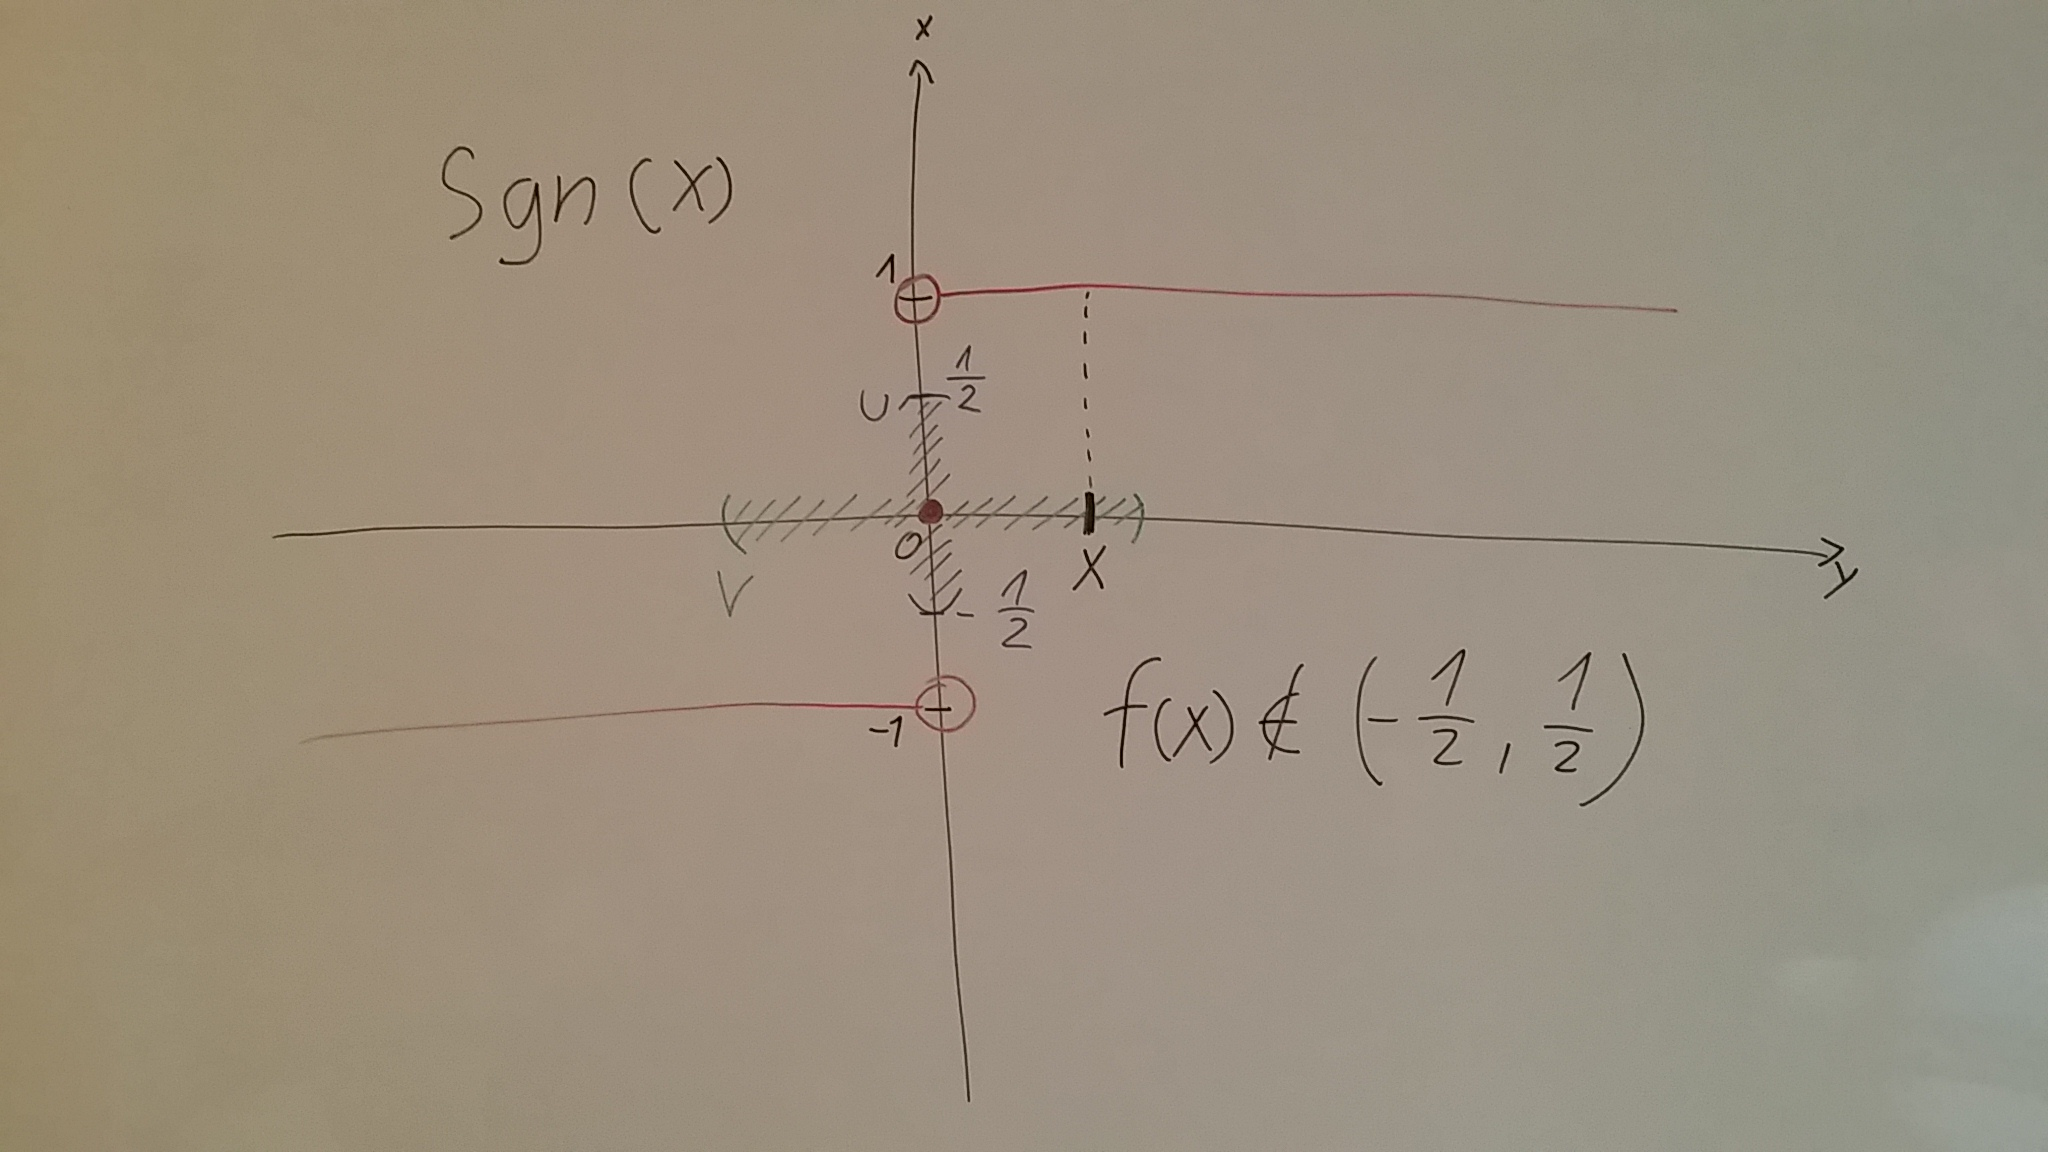
\includegraphics[scale=0.2]{img/sgn}
	\end{center}
	\caption{Príklad nespojitosti sgn v bode 0}
\end{figure}

\subsection{Limita funkcie}
\paragraph{}
Majme topologický priestor $X$, Hausdorfov topologický priestor $Y$, zobrazenie $f:A \subseteq X \rightarrow Y$ a bod $x_{0}$ ktorý je hromadným bodom množiny $A$. \textbf{Limitou zobrazenia} $f$ v bode $x_{0}$ nazývame prvok $y_{0} \in Y$ taký, že zobrazenie: 
\begin{center}
	$f'(x) = \left\{ \begin{array}{ll} f(x), ak\hspace{0.35cm} x \neq x_{0} \\ \hspace{0.45cm} y_{0}, ak \hspace{0.35cm}x = x_{0} \\ \end{array} \right.$
\end{center}
je spojité v bode $x_{0}$. Ak je $y_{0}$ limitou zobrazenia $f$ v bode $x_{0}$, píšeme $y_{0}=\lim_{x \to x_{0}} f(x)$. Dalo by sa povedať že limita je taký prvok priestoru $Y$, ktorý je treba funkcii $f$ v bode $x_{0}$ dodefinovať(predefinovať), aby bola v $x_{0}$ spojitá.

\begin{result}
	(\textbf{$\epsilon -\delta$ kritérium limity po prvé}) Funkcia $f: X \subseteq \mathds{R} \rightarrow \mathds{R}$ má v hromadnom bode $x_{0}$ množiny $X$ limitu $y_{0}$, práve vtedy keď ku každému číslu $\epsilon>0$ existuje číslo $\delta>0$ také, že pre každé $x \in X, x\neq x_{0}$, ktoré splňuje $|x-x_{0}|<\delta$, platí $|f(x)-y_{0}|<\epsilon$.
\end{result}

\begin{sentence}
	Každé zobrazenie má v dannom bode najviac jednu limitu. (Dokaz sporom, predpokladáme že funkcia má v nejakom bode 2 limity a na základe definície prídeme ku sporu).
\end{sentence}
\vspace{-0.8cm}
\paragraph{}
Teraz si zavedieme \textbf{rozšírenú množinu reálnych čísel}. Nazývame ňou množinu \\ $\mathds{R}' = R \cup \{-\infty, \infty\}$, kde $-\infty $ a $ \infty$ sú ľubovolné dva rozličné prvky, takzvané \textbf{nevlastné body}, ktoré niesú reálne čísla.
\vspace{-0.5cm}
\paragraph{}
Limity funkcií reálnej premennej vždy uvažujeme na množine $\mathds{R}'$. V limite $\lim_{x \to x_{0}} f(x)$ teda može byť $x_{0}=-\infty $ alebo $ x_{0}=\infty$(ak sú $-\infty$ alebo $\infty$ hromadným bodom definičného oboru funkcie $f$) a može nám tiež vyjsť že $\lim_{x \to x_{0}} f(x) = -\infty$ alebo $\lim_{x \to x_{0}} f(x) = \infty$. V prvom prípade hovoríme o \textbf{limite v nevlastnom bode}, v druhom o \textbf{nevlastnej limite}.

\begin{result}
	(\textbf{$\epsilon -\delta$ kritérium limity po druhé}) Nech je $X \subseteq \mathds{R}$ taká, že $\infty$ je jej hromadný bod, $f: X \subseteq \mathds{R} \rightarrow \mathds{R}$ funkcia. Prvok $y_{0} \in \mathds{R}'$ je limitou $f$ v bode $\infty$, práve vtedy keď ku každému číslu $\epsilon>0$ existuje číslo $\delta>0$ také, že pre každé $x \in X$, ktoré splňuje $x>\delta$, platí $|f(x)-y_{0}|<\epsilon$, ak je $y_{0}\in \mathds{R}$; poprípade $f(x)>\epsilon$, ak je $y_{0}=\infty$; poprípade $f(x)<-\epsilon$, ak je $y_{0}=-\infty$. Podbne pre limitu v bode $-\infty$.
\end{result}
\vspace{-0.8cm}
\paragraph{\textbf{Majme limity:}}

\begin{enumerate}
	\item $\lim_{x \to x_{0}} f(x)$ pre $x<x_{0}$
	\item $\lim_{x \to x_{0}} f(x)$ pre $x>x_{0}$
\end{enumerate}

Limitu 1 nazývame \textbf{limitou zľava} (značíme: $\lim_{x \to x_{0}^{-}} f(x)$) a limitu 2 nazývame \textbf{limitou zprava} (značíme: $\lim_{x \to x_{0}^{+}} f(x)$).

\begin{figure}[ht]
	\begin{center}
		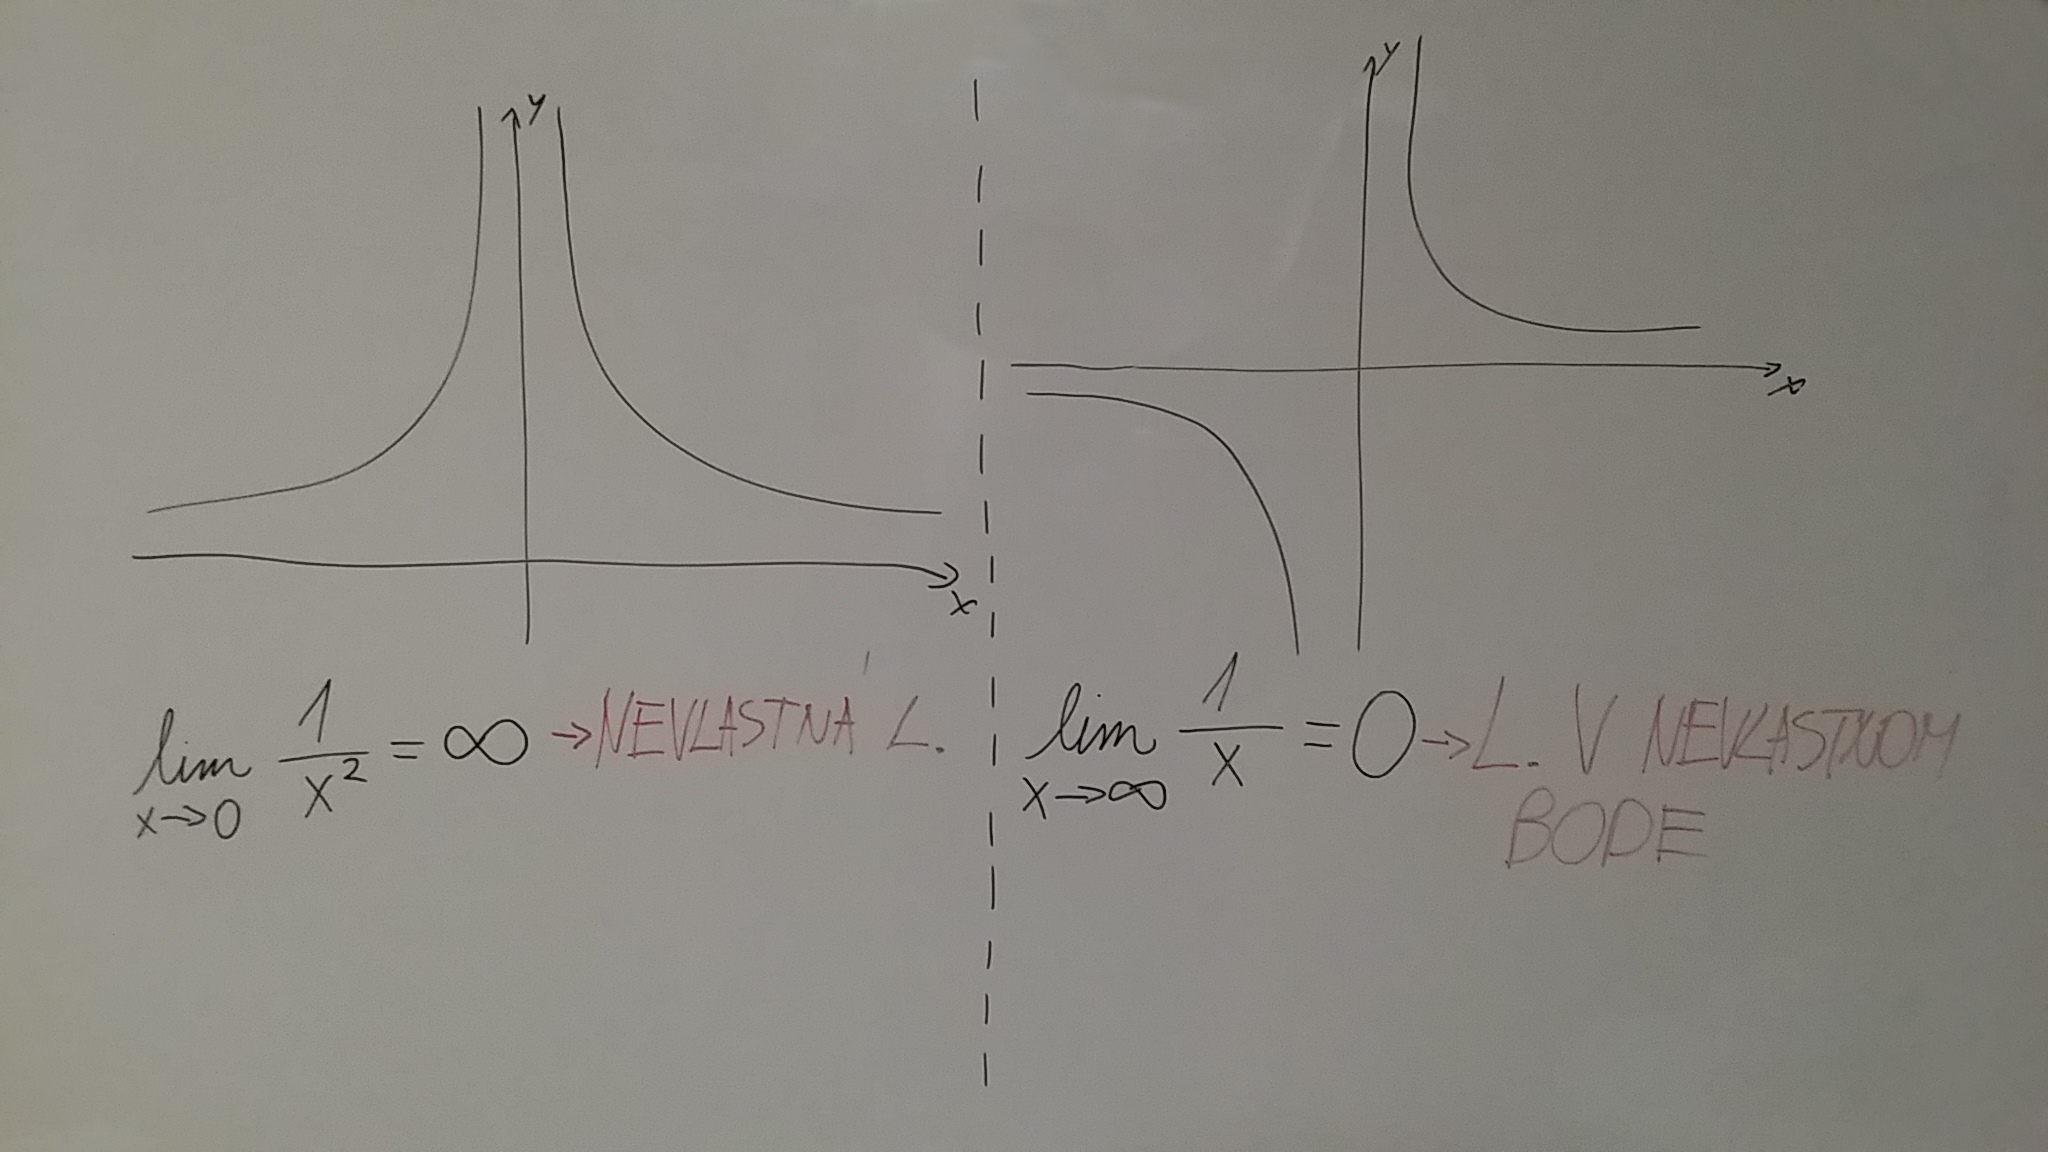
\includegraphics[scale=0.148]{img/limits}
	\end{center}
	\caption{Príklady limít}
\end{figure}

\section{Diferenciálny počet v $\mathds{R}$}
\paragraph{}
Táto sekcia obsahuje vysvetlenie pojmu \textbf{derivácia funkcie}, jej \textbf{geometrický význam} a základné \textbf{vety diferenciálneho počtu} v $\mathds{R}$. Ďalej obsahuje využitie derviácií pri hľadaní extrémov funkcie, odahade hodnoty funkcie \dots (\textbf{Vyšetrovanie priebehu funkcie}).

\subsection{Derivácia a jej geometrický význam}
\paragraph{}

Postupnými úvahami sa pokúsime definovať pojem \textbf{tečny ku grafu funkcie}. Uvažujme funkciu $f: I \subseteq \mathds{R} \rightarrow \mathds{R}$ definovanú na otvorenom intervale $I$. Zvolme si ľubovolný bod $x_{0}\in I$ a kladné celé čislo $h \in \mathds{R}$ tak, aby $x_{0}+h\in I$. Označme si $P=(x_{0}, f(x_{0}))$ a $Q=(x_{0}+h, f(x_{0}+h))$ ako 2 body na grafe funkcie $f$. Na základe vety ktorá je uvedená v definícii \ref{priamka} vieme, že grafom afinnej funkcie je \textbf{priamka}, pozri obrázok \ref{derivacia}. Predstavme si priamku, ktorá prechádza nami definovanými bodmi $P$ a $Q$. Táto priamka je grafom afinnej funkcie $g:\mathds{R} \rightarrow \mathds{R}$ s predpisom:
\begin{center}
	$g(x)=\frac{f(x_{0}+h)-f(x_{0})}{h}(x-x_{0})+f(x_{0})$
\end{center}
Smernica tejto priamky je $g(x)=\frac{f(x_{0}+h)-f(x_{0})}{h}$. Limitu smerníc takýchto priamok (ak existuje), nazývame \textbf{derivácia funkcie} $f$ v bode $x_{0}$ a značíme ju $f'(x_{0})$. Formálne:
\vspace{-0.75cm}
\begin{center}
	$$f'(x_{0})= \lim_{h\rightarrow 0}\frac{f(x_{0}+h)-f(x_{0})}{h} \quad alebo \quad f'(x_{0})= \lim_{x\rightarrow x_{0}}\frac{f(x)-f(x_{0})}{x-x_{0}}$$
\end{center}
Ak nahradíme limitu limitou zľava(zprava) dostaneme \textbf{deriváciu zľava(zprava)} funkcie $f$ v bode $x_{0}$. Značíme ju $f'_{-}(x_{0})\enspace (f'_{+}(x_{0}))$. Ak je limita nevlastná, hovoríme že $f$ má v bode $x_{0}$ \textbf{nevlastnú deriváciu} (obdobne pre vlastnú deriváciu). 

\begin{figure}[ht]
	\begin{center}
		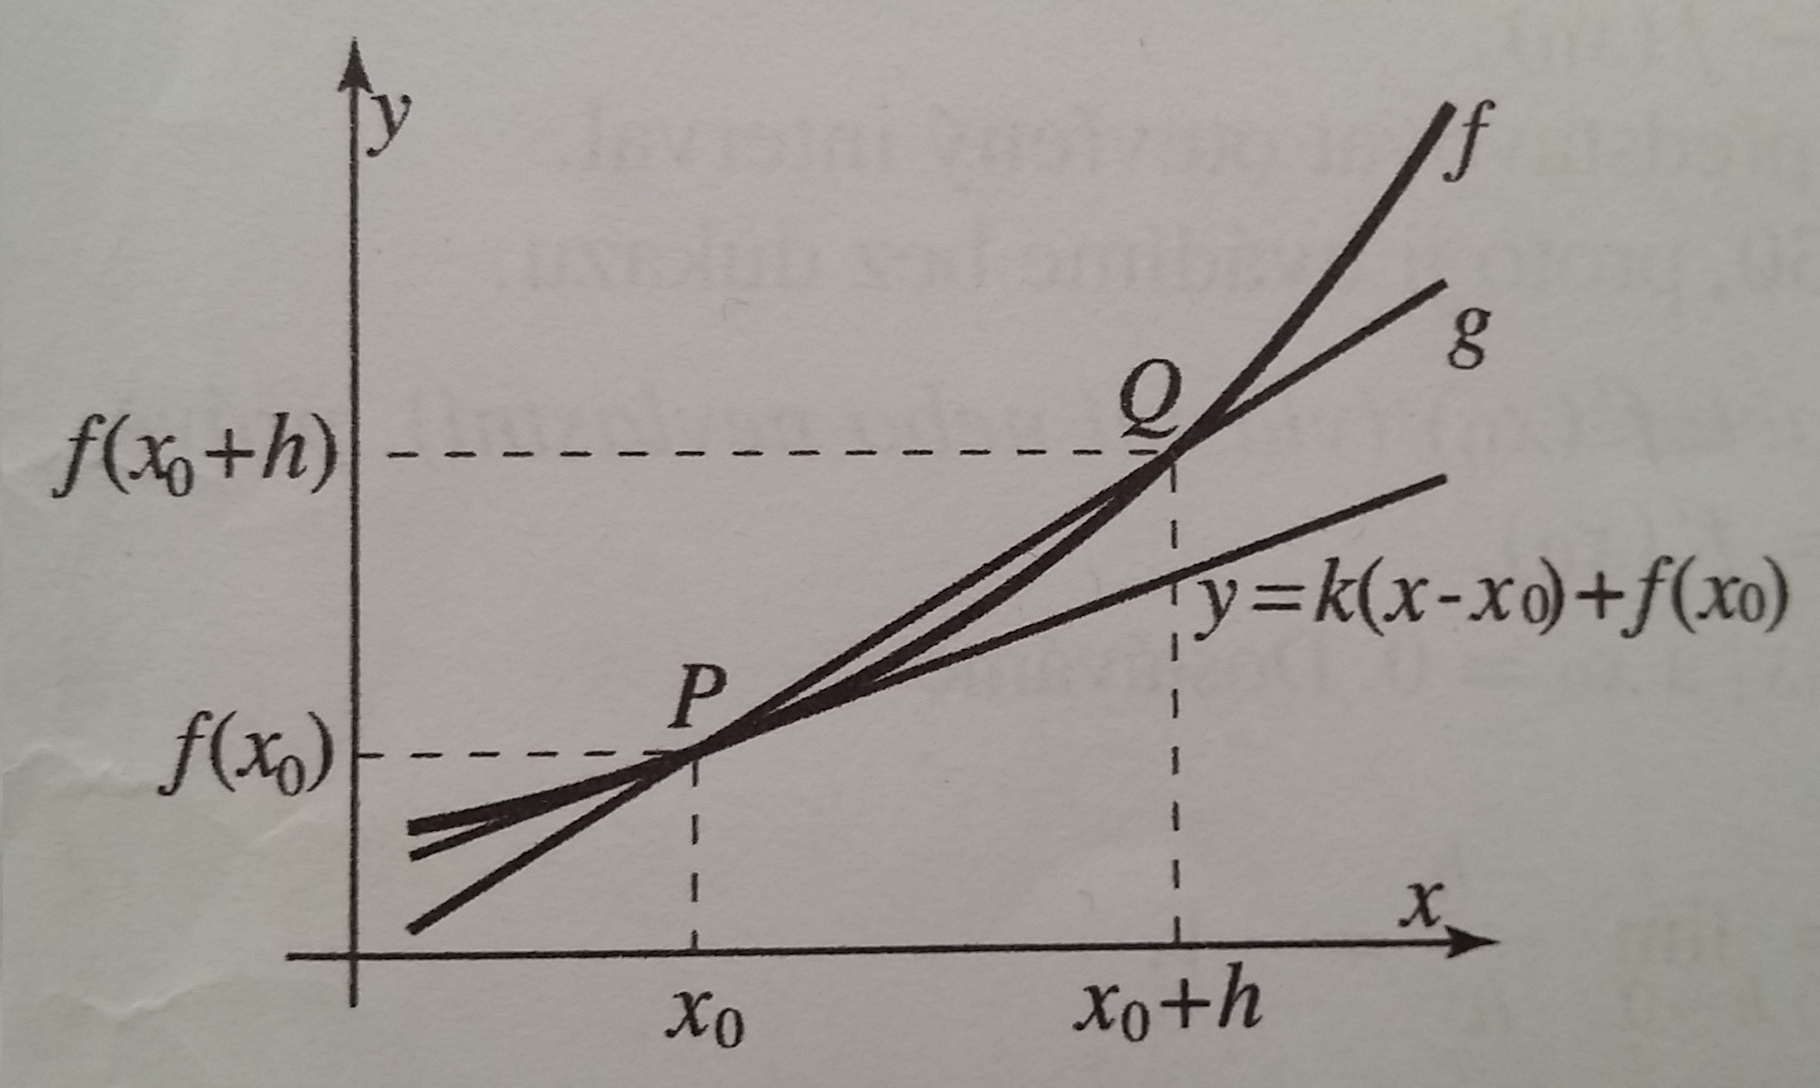
\includegraphics[scale=0.16]{img/derivacia}
	\end{center}
	\caption{Grafické znázornenie úvah o derivácii\label{derivacia}}
\end{figure}

\paragraph{} Označenie derivácie $f'(x_{0})$, pripomína hodnotu nejakej funkcie (zámerne). Majme funkciu $f: J \subseteq \mathds{R} \rightarrow \mathds{R}$. Ak je $X\subseteq J$ je množina obsahujúca všetky body, v ktorých má $f$ vlastnú deriváciu. Potom funkciu $f':X\rightarrow \mathds{R}$, ktorá bodu $X$ priradí deriváciu funkcie $f$ v tomto bode, nazveme \textbf{derivácia funkcie}.

\begin{example}
	Ak je $f$ konštantná funkcia, potom jej derivácia $f'=0$. Konkrétne $f(x)=c$ je konštantná funkcia. Stačí dosadiť\dots \\ $$f'(x_{0})= \lim_{h\rightarrow 0}\frac{f(x_{0}+h)-f(x_{0})}{h}=\lim_{h\rightarrow 0}\frac{c-c}{h}=\lim_{h\rightarrow 0}\frac{0}{h}=0$$ \dots a preto je derivácia konštanty rovná 0.
\end{example}

\begin{definition}
	Teraz už máme dostatočný aparát na zadefinovanie pojmu tečna. Priamka prechádzajúca bodom $(x_{0}, f(x_{0}))$ majúca smernicu $f'(x_{0})$ je \textbf{tečna ku grafu funkcie} $f$ v bode $(x_{0}, f(x_{0}))$.
\end{definition}

\begin{sentence}
	Funkcia $f:J\rightarrow \mathds{R}$ má v bode $x_{0}\in J$ deriváciu $f'(x_{0})$ práve vtedy, keď existujú $f'_{-}(x_{0})$, $f'_{+}(x_{0})$ a platí $f'_{-}(x_{0})=f'_{+}(x_{0})=f'(x_{0})$. (Antidebilne povedané, funkcia má v bode deriváciu, ak má v danom bode deriváciu zľava aj zprava, ktoré sa rovnajú derivácii funkcie v danom bode) Príklad nasleduje \dots
\end{sentence}

\begin{example}
	Za funkciu si zvolme absolútnu hodnotu a ideme hľadať deriváciu v bode 0 takže: $f(x)=|x|$ a $x_{0}=0$. (Fúfam že každý vie ako vyzerá funkcia absolútnej hodnoty \dots kto nie, tak gooooogle!) Dostávame: $$f'_{-}(0)= \lim_{h\rightarrow 0_{-}}\frac{f(x_{0}+h)-f(x_{0})}{h}=\lim_{h\rightarrow 0_{-}}\frac{|h|}{h}=\lim_{h\rightarrow 0_{-}}\frac{-h}{h}=-1$$ $$f'_{+}(0)= \lim_{h\rightarrow 0_{+}}\frac{f(x_{0}+h)-f(x_{0})}{h}=\lim_{h\rightarrow 0_{+}}\frac{|h|}{h}=\lim_{h\rightarrow 0_{+}}\frac{h}{h}=1$$ Ako vidíme tak absolútna hodnota ma deriváciu zľava v bode 0 rovnú -1 a zprava rovnú 1. Preto na základe predchádzajúcej vety \textbf{nemá} deriváciu v bode 0.
\end{example}

\begin{sentence}
	Majme funkcie $f, g:J\subseteq \mathds{R} \rightarrow \mathds{R}$ majúce deriváciu v $x_{0}\in J$ a $c\in \mathds{R}$. Potom:
	\begin{enumerate}
		\item $(f+g)'(x_{0})=f'(x_{0})+g'(x_{0})$
		\item $(fg)'(x_{0})=f'(x_{0})g(x_{0})+f(x_{0})g'(x_{0})$
		\item $(cf)'(x_{0})=cf'(x_{0})$
	\end{enumerate}
\end{sentence}

\begin{sentence}
	\textbf{(Derivácia zloženej funkcie)} Nech $f:J\rightarrow \mathds{R}, g:I\rightarrow J, x_{0}\in I$ a nech existujú vlastné derivácie $g'(x_{0})$ a $f'(g(x_{0}))$. Potom existuje vlastná derivácia $(f\circ g)'(x_{0})$ a platí $(f\circ g)'(x_{0})=f'(g(x_{0}))\cdot g'(x_{0})$.
\end{sentence}

\begin{result}
	Majme $f, g:J\subseteq \mathds{R} \rightarrow \mathds{R}$ funkcie majúce driváciu v $x_{0}\in J$ a $g(x_{0})\neq 0$. Potom: $$\bigg(\frac{f}{g}\bigg)'(x_{0})=\frac{f'(x_{0})g(x_{0})-f(x_{0})g'(x_{0})}{g^{2}(x_{0})}$$.
\end{result}

\begin{sentence}
	\textbf{(Derivácia inverznej funkcie)} Nech $f:J\rightarrow I\subseteq\mathds{R}$ je spojitá rastúca alebo klesajúca, $x_{0}\in J, f^{-1}:I\rightarrow J$ je inverzia $f$. Ak existuje vlastná $f'(x_{0})\neq 0$, potom existuje vlastná $(f^{-1})'(f(x_{0}))$ a platí:$$(f^{-1})'(f(x_{0}))=\frac{1}{f'(x_{0})}$$.
\end{sentence}

\begin{definition}
	Uvažujme funkciu $f:J\rightarrow \mathds{R}$ a $x_{0}\in J$. Lineárne homogénne zobrazenie $A:\mathds{R}\rightarrow \mathds{R}$ nazývame \textbf{diferenciál funkcie} $f$ v bode $x_{0}$, ak $$\lim_{h\rightarrow 0}\frac{f(x_{0}+h) - f(x_{0})-A(h)}{h}=0$$ Diferencál funkcie $f$ v bode $x_{0}$ označujeme $df(x_{0})$.
\end{definition}

\subsection{Vyšetrovanie priebehu funkcie}
\paragraph{}
Pomocou derivácií možeme vyšetriť priebeh funkcie. Definovali sme tečnu ku grafu funkcie. Strmosť tečny nám určuje, ako moc sa hodnoty menia. Derivácia v bode extrému je rovná 0, v tom istom bode je tečna rovnobežná s osou $x$ (toto je jeden z ukazovatelov že sa nachádzame v extréme). Pozri obrázok \ref{tecna}.

\begin{figure}[ht]
	\begin{center}
		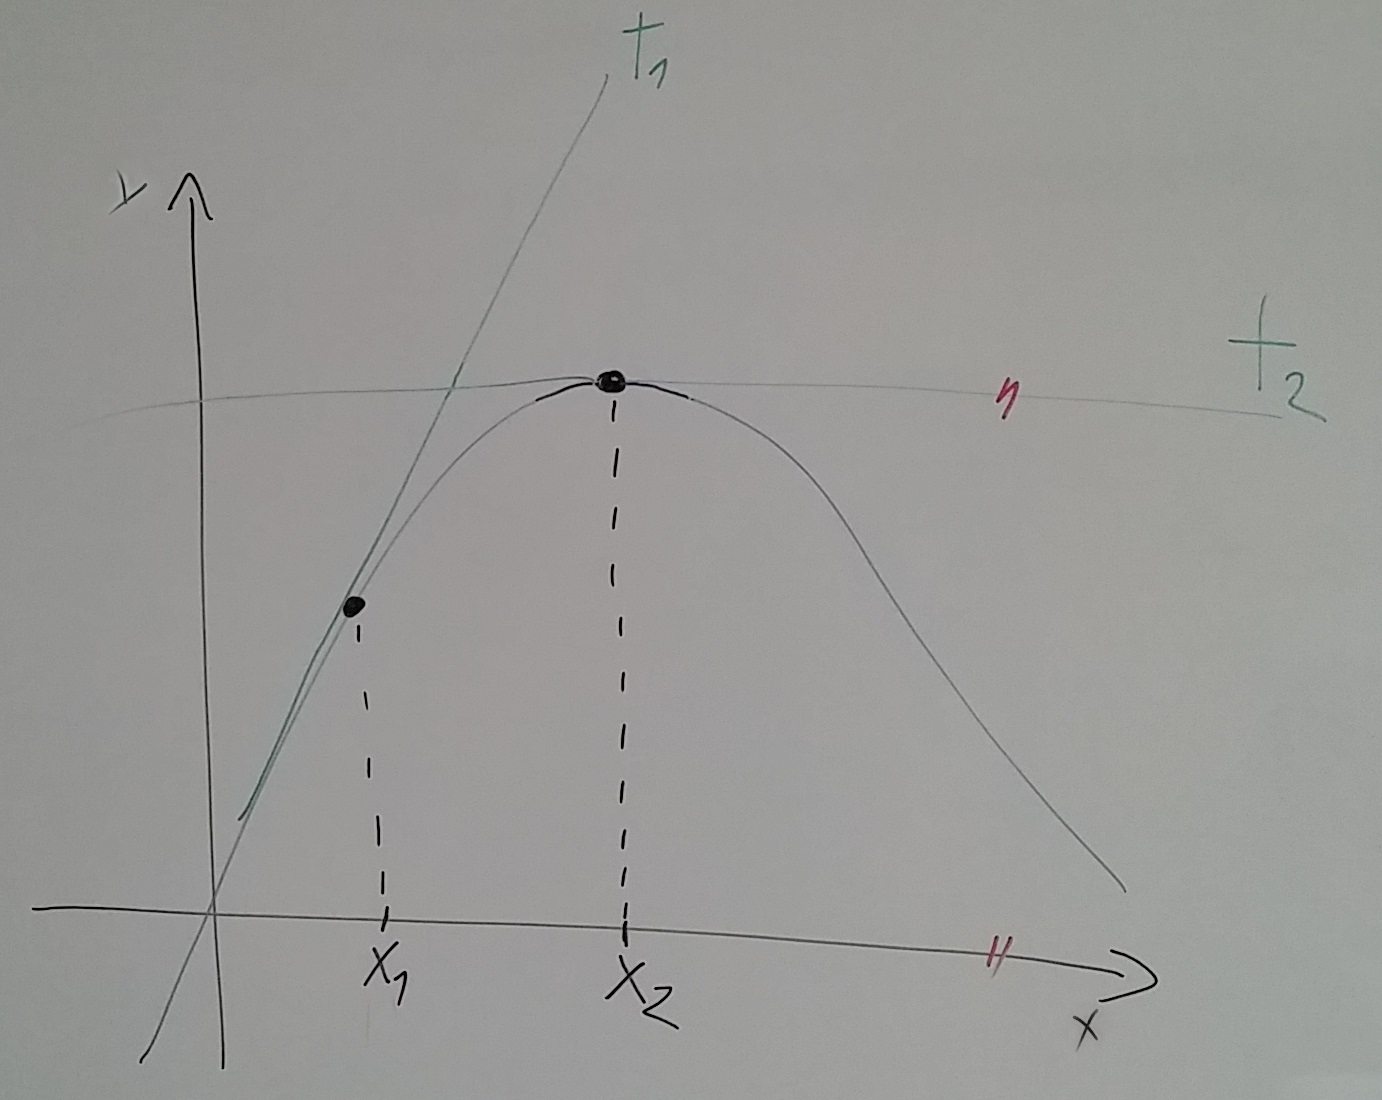
\includegraphics[scale=0.24]{img/tecna}
	\end{center}
	\caption{Tečna ku grafu funkcie v bode $x_{1}$ a $x_{2}$, v bode $x_{1}$ vidíme že tečna je strmá(hodnoty sa menia výrazne), v bode $x_{2}$ vidíme že tečna je rovnobežná s osou x, takže sa nachádzame v extréme (derivácia by v $x_{2}$ bola rovná 0)\label{tecna}}
\end{figure}

\subsubsection{Extrémy}
\paragraph{}
Nech $f:X\subseteq \mathds{R}\rightarrow \mathds{R}$. Povedzme že funkcia $f$ je \textbf{rastúca (respektívne klesajúca, nerastúca, neklesajúca)} v bode $x_{0}\in X$, ak existuje okolie $(x_{0}-\delta, x_{0}+\delta)$ bodu $x_{0}$ také, že $f((x_{0}-\delta, x_{0})\cap X)<f(x_{0})<f((x_{0}, x_{0}+\delta)\cap X)$ (respektívne $f((x_{0}-\delta, x_{0})\cap X)>f(x_{0})>f((x_{0}, x_{0}+\delta)\cap X)$, $f((x_{0}-\delta, x_{0})\cap X)\geq f(x_{0})\geq f((x_{0}, x_{0}+\delta)\cap X)$, $f((x_{0}-\delta, x_{0})\cap X)\leq f(x_{0})\leq f((x_{0}, x_{0}+\delta)\cap X)$). \paragraph{}
Povedzme, že funkcia $f$ nabýva v $x_{0}$ \textbf{lokálne maxima (minima)} ak existuje okolie $U$ bodu $x_{0}$ také, že $f|_{U\cap X}$ (tento zápis znamená zúženie funkcie $f$ na okolie $U$) nabýva v $x_{0}$ maxima (minima).

\begin{sentence}
	Majme $f:J\rightarrow \mathds{R}$, potom:
	\begin{enumerate}
		\item Ak je $f'(x_{0})>0$ (poprípade ak je $f'(x_{0})=\infty$), potom je $f$ v bode $x_{0}$ \textbf{rastúca}.
		\item Ak je $f'(x_{0})<0$ (poprípade ak je $f'(x_{0})=-\infty$), potom je $f$ v bode $x_{0}$ \textbf{klesajúca}.
	\end{enumerate}
\end{sentence}

\begin{result}
	\label{dosledok1}
	Ak je $x_{0}\in J$ bodom extrému funkcie $f:J\rightarrow \mathds{R}$ a existuje $f'(x_{0})$, potom $f'(x_{0})=0$ (ako sme tvrdili v úvode).
\end{result}

\subsection{Základné vety diferenciálneho počtu}
\begin{sentence}
	\textbf{(Rolleova)} Majme $f:[a,b]\rightarrow \mathds{R}$ spojitá funkcia majúca deriváciu (vlastnú alebo nevlastnú) v každom vnútornom bode $[a,b]$. Ak $f(a)=f(b)$, potom existuje $c\in (a, b)$ také, že$f'(c)=0$.
\end{sentence}
\paragraph{}
\textbf{D:} Ak je $f$ konštantná, potom $c$ je ľubovolný bod intervalu $(a, b)$. Uvažujme 2 rozne prípady. \textbf{Prvý:} Ak existuje bod v (a, b), v ktorom funkcia $f$ nabýva hodnoty vačšej než $f(a)$, potom vezmeme za $c$ bod v ktorom funkcia $f$ nabýva na $[a, b]$ svojho maxima. Taký bod existovať bude (na základe vety 4.9 \dots neviem kde ju doc. Krupka dal ale ja som ju nenašiel) a bude rozny od $a, b$, pretože funkcia $f$ nabýva hodnoty vaščej než $f(a)$ v nejakom bode $(a, b)$. Ostáva ukázať že $f'(c)=0$. To ale plynie z dosledku číslo \ref{dosledok1}.

\begin{sentence}
	\textbf{\textbf{(Lagrangeova veta o strednej hodnote)}} Majme $f:[a,b]\rightarrow \mathds{R}$ spojitá funkcia majúca deriváciu (vlastnú alebo nevlastnú) v každom vnútornom bode $[a,b]$. Potom existuje $c\in (a, b)$ také, že $f'(c)=\frac{f(b)-f(a)}{b-a}$. (Používa sa k odhadu, ako rýchlo funkcia rastie)
\end{sentence}

\paragraph{}
\textbf{D:} Vetu dokážeme pomocou Rolleovej vety tak, že ju aplikujeme na rozdiel funkcie $f$ a afinnej funkcie $g$ prechádzajúcej bodmi $(a, f(a)) a (b, f(b))$. Uvažujme teda funkciu $F:[a, b]\rightarrow \mathds{R}$ s predpisom $F(x)=f(x)-\frac{f(b)-f(a)}{b-a}(x-a)-f(a)$. Táto funkcia spĺňa všetky predpoklady Rolleovej vety. Preto existuje $c\in (a, b)$ také, že $F'(c)=0$. Pretože $F(x)=f(x)-\frac{f(b)-f(a)}{b-a}$ pre $x=c$ dostávame $F(c)=f(c)-\frac{f(b)-f(a)}{b-a}=0$.

\begin{figure}[H]
	\begin{center}
		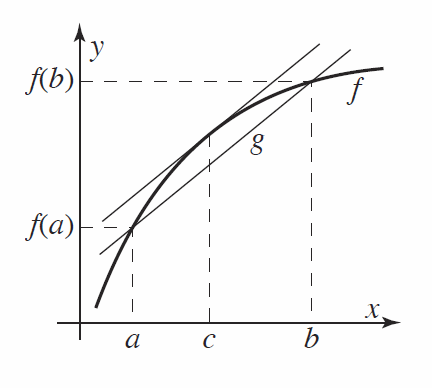
\includegraphics[scale=0.6]{img/lagrangeova_veta}
	\end{center}
	\caption{Lagrangeova veta}
\end{figure}

\begin{result}
	Majme $f, g:[a, b]\rightarrow \mathds{R}$ spojité funkcie. Ak platí že $f' = g'$, potom existuje $c\in\mathds{R}$ také, že $f=g+c$. (Inak povedané, funkcie s rovnakou deriváciou sa na intervale líšia iba o konštantu.)
\end{result}

\begin{sentence}
	\textbf{(Couchova veta o strednej hodnote)} Majme $f, g:[a, b]\rightarrow \mathds{R}$ spojité funkcie a nech existuje v každom bode $x\in (a, b)$ derivácia $f'(x)$ (vlastná alebo nevlastná) a vlastná derivácia $g'(x)\neq 0$. Potom exituje $x\in (a, b)$ také, že $\frac{f'(c)}{g'(c)}=\frac{f(b)-f(a)}{g(b)-g(a)}$.
\end{sentence}
\paragraph{}
\textbf{D:} Vetu dokážeme obdobným sposobom ako tú predchádzajúcu. Najprv, pretože $g'(x)\neq 0$ na $(a, b)$, podľa Lagrangeovej vety máme, že $g(a)\neq g(b)$. Definujeme funkciu \\ $F:[a, b]\rightarrow \mathds{R}$ s predpisom $F(x)=(f(x)-f(a))(g(b)-g(a))-(g(x)-g(a))(f(b)-f(a))$. Táto funkcia spĺňa podmienky Rolleovej vety a preto existuje $c\in (a, b)$ také, že $F'(c)=0$, teda $F'(c)= f'(x)(g(b)-g(a))-g'(c)(f(b)-f(a))=0$.

\begin{example}
	Uvažujme funkciu $f=ln$ na intervale $[a, b]=[5, 10]$. Podľa vety o strednej hodnote existuje $c\in(5, 10)$ také, že $(10-5)ln'(c)=5/c=ln 10 - ln 5=ln2$. Pretože $5<c<10$, znamená to, že $\frac{5}{10}<5/c=ln2<\frac{5}{5}$. Dostávame prvý odhad funkcie $ln$ v bode 2: $\frac{1}{2}<ln2<1$. Pokračujme ďalej, z nerovnice $1<2ln2$ a z monotonie funkcie $exp$ dostaneme $e=exp(1)<exp(2ln2)=4$. Číslo $e$ je teda menšie ako 4.
\end{example}

\section{Postupnosti a ich limity}
\subsection{Postupnosti}
\paragraph{}
Ako \textbf{postupnosť} sa označuje usporiadný súbor matematických objektovy očíslovaných spravidla prirodzenými číslam. Postupnosť je možné definovať  ako zobrazenie z množiny prirodzených do ľubovolnej množiny. Členmi postupnosť možu byť čísla (číselné postupnosti), funkcie (funkčné postupnosti), množiny \dots číslená postupnosť priraďuje každému $n\in \mathds{N}$ číslo $a_{n}$ (v prípade funkčnej postupnosti to je $f_{n}(x)$). Postupnosť obvykle značíme $(a_{n})_{n=1}^{\infty}$. Postupnosť može byť vyjedrená aj výrazom na výpočet n-tého člena postupnosti $a_{n}$ (napr. $a_{n}=\frac{n}{n+1}$ odpovedá postupnosti : $a_{1}=\frac{1}{2}$, $a_{2}=\frac{2}{3}$, $a_{3}=\frac{3}{4}$ \dots). Postupnosť možeme zadať aj rekurentne (ďaľší člen postupnosti sa vypočíta pomocou predchádzajúcich členov). Rekurentne je zadaná napr. \textbf{Fibonacciho postupnosť} a to nasledovne: $a_{1}=1$, $a_{2}=1$, $a_{n+2}=a_{n}+a_{n+1}$.

\subsection{Vlastnosti postupností}
\paragraph{}
Kedže postupnosť je možné zadefinovať ako zobrazenie, tak bude mať rovnaké vlastnosti ako zobrazenie. Postupnosť je:
\begin{enumerate}
	\item \textbf{rastúca}, ak pre všetky $i$ platí, $a_{i}>a_{i-1}$
	\item \textbf{nerastúca}, ak pre všetky $i$ platí, $a_{i}\leq a_{i-1}$
	\item \textbf{klesajúca}, ak pre všetky $i$ platí, $a_{i}<a_{i-1}$
	\item \textbf{neklesajúca}, ak pre všetky $i$ platí, $a_{i}\geq a_{i-1}$
	\item \textbf{zhora ohraničená} na množine $A$, ak existuje taká $L\subseteq A$, že pre všetky $i$ platí $a_{i}\leq L$ (tým sú myslené prvky z $L$)
	\item \textbf{zdola ohraničená} na množine $A$, ak existuje taká $L\subseteq A$, že pre všetky $i$ platí $a_{i}\geq L$	
\end{enumerate}

Ak je postupnosť nerastúca alebo neklesajúca, hovoríme, že je \textbf{monotónna}. Ak je rastúca alebo klesajúca hovorýme že je \textbf{rýdzo monotónna}. Ak je postupnosť zároveň zhora aj zdola ohraničená, hovoríme že je \textbf{ohraničená}. Ak sa v ľubovolne malom $\epsilon$ - okolí bodu $b$ na intervale $(b-\epsilon , b+\epsilon )$ nachádza nekonečne veľa bodov postupnosti $(a_{n})$, potom bod $b$ nazývame \textbf{hromadným bodom postupnosti} $(a_{n})$.

\subsection{Príklady postupností}
\subsubsection{Aritmetická postupnosť}
\paragraph{}
Je druh postupnosti kde je stály rozdiel medzi susednými členmi postupnosti. Tento rozdiel sa volá diferencia a značí sa \textbf{d}. Ďalej su to 3-prdele vzorcov na počítanie s aritmetickou postupnosťou (tie ale uvádzať nebudeme).

\begin{example}
	Majme aritmetickú postupnosť zadanú prvým členom a diferenciou: $a_{1}=5$, $d=5$. Vypočítajte $a_{2}$, $a_{3}$. (Je to hard \dots berte kalkulačky súdruhovia).
\end{example}

\subsubsection{Geometrická postupnosť}
\paragraph{}
Druh postupnosti kde je každý člen (okrem prvého) stálym násobkom predchádzjúceho člena. Tento násobok sa volá kvocient a značí sa \textbf{q}. Je možné ju chápať ako zúženie exponenciálnej funkcie na obor prirodzených čísel. Obsahuje podobné množstvo vzorcov ako aritmetická \dots

\begin{example}
	Majme geometrickú postupnosť zadanú prvým členom a kvocientom: $a_{1}=2$, $d=2$. Vypočítajte $a_{2}$, $a_{3}$, $a_{4}$. ($a_{2}=4$, $a_{3}=8$, $a_{4}=16$).
\end{example}

\subsubsection{Fibonacciho postupnosť}
Všetkým známa.

\begin{figure}[H]
	\begin{center}
		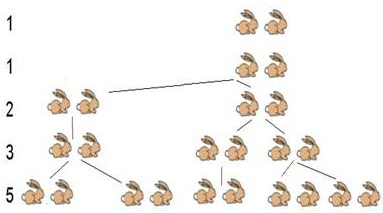
\includegraphics[scale=1]{img/fibonacci}
	\end{center}
	\caption{Fibonacciho postupnosť ilustratívne}
\end{figure}

\subsection{Limita postupnosti}
\begin{definition}
	Postupnosť $(a_{n})_{n=1}^{\infty}$ má \textbf{limitu} $L$, ak sa jej hodnotami može k $L$ priblížiť. Teda pre každé kladné číslo $\epsilon$ platí, že existuje nejaký člen postupnosti od ktorej sú už jej hodnoty od $L$ vzdialené menej než $\epsilon$. Formálne zapísané, ak pre pre každéb $\epsilon>0$ existuje $n_{0}$ také, že pre každé $n>n_{0}$ platí, že $|a_{n}-L|<\epsilon$.
\end{definition}

\paragraph{}
Ak k ľubovolnému $\epsilon>0$ existuje $n_{0}$ také, že pre každé $n>n_{0}$ platí, že $|a_{n}-L|<\epsilon$ hovoríme, že postupnosť $(a_{n})$ má \textbf{vlastnú a konečnú limitu L}. Inak povedané postupnosť \textbf{konverguje} k $L$. To že postupnosť konverguje k $L$ zapisujeme: $$\lim_{n\rightarrow \infty} a_{n}=L$$. Ak má postupnosť vlastnú limitu, tak postupnosť označujeme ako \textbf{konvergentnú}. V opačnom prípade hovoríme o \textbf{divergentnej} postupnosti. O postupnosti hovríme že je:

\begin{enumerate}
	\item \textbf{konvergentná}, ak má vlastnú limitu
	\item \textbf{divergentná}, ak má nevlastnú limitu $+\infty$ alebo $-\infty$, je oscilujúca alebo nemá limitu
	\item \textbf{oscilujúca}, ak nemá vlastnú limitu ani nevlastnú limitu
\end{enumerate}

\section{Číselné rady, konvergencia a súčty, kritéria konvergencie}
\paragraph{}
Majme postupnosť $(x_{n})$ reálnych čísel. \textbf{Nekonečným radom} určeným postupnosťou $(x_{n})$ rozumieme symbol $\sum x_{n}$. Postupnosť $(s_{n})$, ktorej členy su danné predpisom $s_{n}=x_{1} + \dotsm + x_{n}$ (kde $n=1, 2, 3 \dots$), nazývame \textbf{postupnosťou čiastočných súčtov radu} $\sum x_{n}$. Ak postupnosť čiastočných súčtov radu $\sum x_{n}$ konverguje, hovoríme o \textbf{konvergentnom rade} a číslo $s_{n}$ nazývame jeho \textbf{súčtom}. V opačnom prípade hovoríme o \textbf{divergentnom rade}. Súčet nekonečného radu $\sum x_{n}$ označujeme rovnako $\sum x_{n}$. Tvrdenie $\sum x_{n}=s$ znamená: Rad $\sum x_{n}$ konverguje a jeho súčtom je $s$. Okrem tohoto zápisu sa používa aj zápis $\sum_{n=1}^{\infty} x_{n}$. Zápis $\sum_{n=k}^{\infty} x_{n}$ znamená $\sum_{n=1}^{\infty} x_{n}+k-1$. V takom prípade budeme používať nasledujúce značenie pre postupnosť čiastočných súčtov radu: $s_{n}=x_{k}+x_{k+1}+\dotsm + x_{k+n-1}$.

\subsection{Príklady radov}
\paragraph{}
Nech $q\in \mathds{R}$. Rad $\sum q^{n-1}$ sa nazýva \textbf{geometrický rad} s kvocientom $q$. Ak je $q\neq 1$, potom pre n-tý člen $s_{n}$ jeho postupnosti čiastočných súčtov platí:$$s_{n}=1+q+q^{2}+q^{3}+\dotsm + q^{n-1}=\frac{1-q}{1-q}(1+q+q^{2}+q^{3}+\dotsm + q^{n-1}) = \frac{1-q^{n}}{1-q}$$
Ak je $q=1$, platí $s_{n}=n$\\
Vidíme teda, že $lim \; s_{n}$ existuje, práve vtedy keď $|q| < 1$, a je rovná $1/(1-q)$. Uvedený rad teda konverguje práve vtedy, keď $|q| < 1$, a v tom prípade platí $\sum q^{n-1}=1/(1-q)$. \paragraph{} Geometrický rad s $q=-1$ sa nazýva \textbf{Grandiho rad}. Rad $\sum 1/n$ sa nazýva \textbf{harmonický rad}. Pre postupnosť $(s_{n})$ jeho čiastočných súčtov platí: $$s_{1}=1$$$$s_{2}=1+\frac{1}{2}$$$$s_{3}=1+\frac{1}{2}+\frac{1}{3}$$$$s_{4}=s_{2}+\frac{1}{3}+\frac{1}{4}>s_{2}+\frac{1}{4}+\frac{1}{4}=s_{2+\frac{1}{2}}$$$$\dotso$$$$s_{2^{n+1}}=s_{2^{n}}+\frac{1}{2}$$
Z toho je možné vysledovať, že harmonický rad diveruje, hoci spĺňa nutnú podmienku konvergencie (uvedená nižšie).

\begin{sentence}
	\textbf{(Cauchyho-Bolzanovo kritérium konvergencie)} Rad $\sum x_{n}$ konverguje, práve vtedy keď ku každému $\epsilon >0$ existuje číslo $n_{0}\in \mathds{N}$ také, že pre každé $n_{1}, n_{2}>n_{0}; \; n_{2}\geq n_{1}$, platí: $|x_{n_{1}}+\dotsm +x_{n_{2}}|<\epsilon$.
\end{sentence}

\begin{result}
	\textbf{(Nutná podmienka konvergencie radu)} Ak rad $\sum x_{n}$ konverguje, potom platí že: $lim \; x_{n}=0$ (Poznámka: zamyslite sa nad geometrickým radom)
\end{result}

\begin{sentence}
	Majme 2 postupnosti reálnych čísel $(x_{n})$, $(y_{n})$ a číslo $c$. Ak rady $\sum x_{n}$ a $\sum y_{n}$ konvergujú, potom konvergujú aj rady $\sum (x_{n}+y_{n})$ a $\sum cx_{n}$ a platí $$\sum (x_{n}+y_{n})=\sum x_{n} + \sum y_{n}$$ $$\sum cx_{n}=c\sum x_{n}$$
\end{sentence}

\begin{sentence}
	Ešte sa tu nachádzajú asi 2 (podľa mňa) menej podstatné vety o konvergencii radov. Ide v nich asi o to že ak sa 2 rady rovnajú a prvý z nich konverguje, tak konverguje aj ten druhý atď \dots
\end{sentence}

\subsection{Rady s nezápornými členmi}
\paragraph{}
Nech $(x_{n})\geq 0$. Postupnosť čiastočných súčtov radu $\sum x_{n}$ je neklesajúca. Konverguje práve vtedy, keď je ohraničená a práve vtedy, keď nejaká jej podpostupnosť. Inak diverguje k $+\infty$.

\begin{sentence}
	\textbf{(Zrovnávacie kritérium)} Nech $\sum x_{n}$ a $\sum y_{n}$ sú rady s nezápornými členmi a nech existuje číslo $n_{0}$ také, že pre každé $n\geq n_{0}$ platí $x_{n}\leq y_{n}$. Potom s konvergencie radu $\sum y_{n}$ plynie konvergencia radu $\sum x_{n}$.
\end{sentence}

\begin{sentence}
	Zase sú tu aj iné vety ... ale myslím že nám chýbať nebudú.
\end{sentence}

\subsection{Alternujúce a absolutne konvergentné rady}
\paragraph{}
Povieme, že rada $\sum x_{n}$ je \textbf{alternujúca}, ak pre každý člen $x_{n}$ má člen $x_{n+1}$ opačné znamienko. Rad $x_{n}$, pre ktorý rad $\sum |x_{n}|$ konverguje, sa nazýva \textbf{absolutne konvergentný}.  Z vety ktorá nasleduje plynie, že absolútne konvergentná rada je konvergentná. Konvergentná rada ktorá nieje absolútne konvergentná, sa nazýva \textbf{neabsolútne konvergentná} (relatívne konvergentná).

\begin{sentence}
	Ak konverguje rad $\sum |x_{n}|$, konverguje aj rad $\sum x_{n}$ a platí $|\sum x_{n}|\leq \sum |x_{n}|$\\ \textbf{D:} (Iba naznačenie) Pre ľubovolné čísla $n_{1}\leq n_{2}$ platí $$|x_{n_{1}}+ \dotsm + x_{n_{2}}|\leq |x_{n_{1}}| + \dotsm + |x_{n_{2}}|$$.
\end{sentence}

\section{Neurčitý a určitý Riemannov integrál}
\paragraph{}
V deriváciách sme hľadali zo zadanej funkcie jej deriváciu. Pomocou integrálov sa rieši opačný problém, takže zo zadanej derivácie určiť povodnú funkciu.

\subsection{Neurčitý integrál}
\paragraph{}
Predpokladajme, že máme danú funkciu $f$, o ktorej vieme, že vznikla derivovaním nejakej funkcie $F$ na intervale $(a, b)$, teda, že $f(x) =F'(x)$ pre každé $x \in (a, b)$. Otázka je: Aká bola povodná funkcia $F$? Funkcia $F$, ktorú hľadáme, sa preto niekedy nazýva \textbf{primitívna funkcia}.

\begin{example}
	Majme funckiu $f(x)=8x^{3}$ pre $x\in (-\infty , \infty)$ Úlohou je nájsť funkciu $F$. ($F=2x^{4}$ pretože pre každé $x\in (-\infty , \infty)$ platí, že $F'(x)=2\cdot 4x^{3}$). 
\end{example}

\begin{definition}
	Nech $(a, b)$ je ľubovolný otvorený interval. Funkcia $F$ sa nazýva primitívnou funkciou k funkcii $f$ na intervale $(a, b)$ ak pre každé $x \in (a, b)$ platí$$f(x)=F'(x)$$
\end{definition}

\begin{sentence}
	Nech funkcia $F$ je primitívnou funkciou k funkcii $f$ na intervale $(a, b)$. Funkcia $G$ je primitívnou funkciou k funkcii $f$ na intervale $(a, b)$ práve vtedy, ak existuje reálne číslo $c$ také, že pre každé $x\in (a, b)$ platí $$G(x)=F(x)+c$$
\end{sentence}

\paragraph{}
To znamená, že primitívne funkcie k rovnakej funkcii $f$ sa môžu líšiť len konštantou. Ak hľadáme ktorúkoľvek z primitívnych funkcií, tak hovoríme, že hľadáme \textbf{neurčitý integrál z funkcie f} a značíme $$\int f(x)dx$$

\paragraph{}
Na základe predchádzajúcej vety možeme neurčitý integrál písať aj v tvare $$\int f(x)dx=F(x)+c$$ kde $F$ je jedna z možných primitívnych funkcií.

\subsubsection{Substitučná metóda (iba informatívne)}
\paragraph{}
Prvá veta o substitučnej metóde umožňuje hľadať neurčité integrály funkcií, ktoré sú
súčinom nejakej zloženej funkcie a derivácie jej vnútornej zložky, napr. integrály typu $$\int (\varphi (x))\cdot \varphi '(x)dx$$

\begin{example}
	Vypočítajte integrál: $$\int \frac{cos(ln\; x)}{x}dx$$ Funkcia $cos(ln \; x)$ je zložená funkcia, pričom $ln \; x$ je vnútorná zložka. Použijeme substitúciu $$t=ln \; x \; \Rightarrow \; dt=\frac{1}{x}dx$$ Pos substitúcii dostaneme $$\int \frac{cos(ln\; x)}{x}dx = \int cos \;t \; dt = sin \;t + c=sin \; (ln \; x)+c$$
\end{example}

\subsubsection{Metóda Per-Partes (iba informatívne)}
\paragraph{}
Aj keď vo všeobecnosti nejaké pravidlo pre integrovanie súčinu dvoch funkcií nemáme, v niektorých prípadoch nám môže pomôcť nasledujúca veta, známa ako veta o metóde "per-partes"(krátko MPP).

\begin{sentence}
	Nech funkcie $u$ a $v$ majú na intervale $(a, b)$ spojité derivácie $u'$ resp. $v'$. Potom na intervale $(a, b)$ platí $$\int u(x) \cdot v'(x)dx = u(x) \cdot v(x) - \int u'(x)\cdot v(x) dx$$ Na pravej strane sme dotsali jednoduhší integrál. Niekedy vieme výsledok z neho určiť priamo, inokedy treba použiť vhodný postup na jeho určenie.
\end{sentence}

\subsection{Určitý Riemannov integrál}
\paragraph{}
Sú 2 sposoby ako zadefinovať určitý Riemannov integrál. Jeden z nich je použitím (Cauchyových) integrálnych súčtov (Ten sme si v MATA nedefinovali) a druhý je použitím \textbf{horných a dolných integrálov}. Nižšie je popísaný druhý sposob.

\paragraph{}
Na začiatok si je treba uvedomiť pri určitom Riemannovom itegrále ide o vyýpočet obsahu polchy pod krivkou nejakej funkcie (Riemannov integrál definujeme v $\mathds{R}$). Predstavme si teda funkciu $f$ obmedzenú na interval $[a, b]$ (Pozri obrázok \ref{int1}). 

\begin{figure}[H]
	\begin{center}
		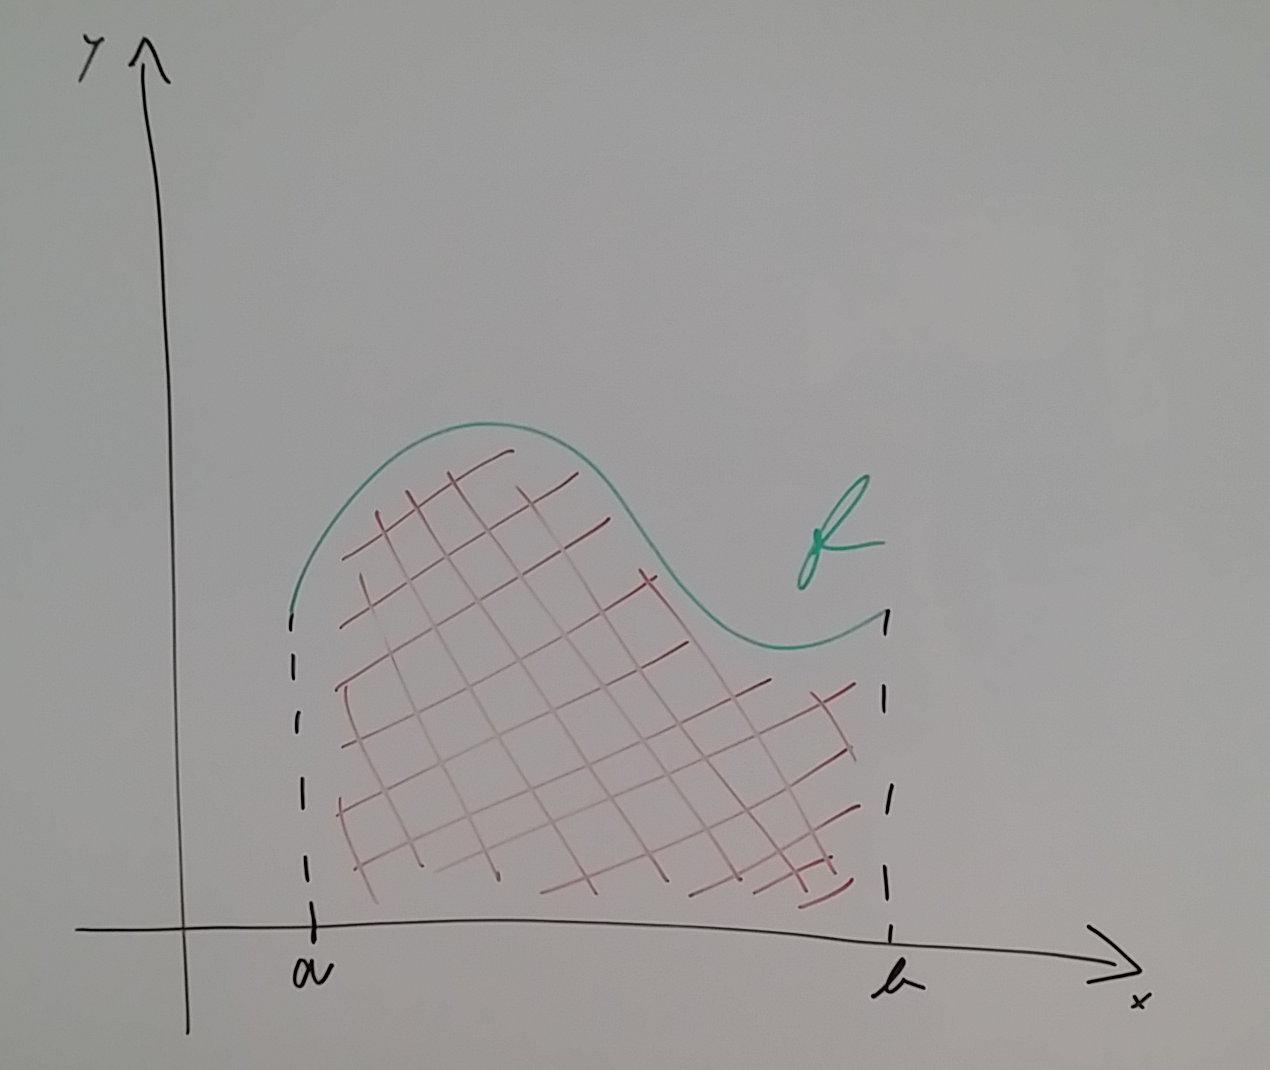
\includegraphics[scale=0.2]{img/int1}
	\end{center}
	\caption{Funkcia $f$ obmedzená na interval $[a, b]$\label{int1}}
\end{figure}

\paragraph{}
Úlohou je teda vypočítať obsah plochy pod krivkou funckie $f$ obmedzenú na interval $[a, b]$. Interval $[a, b]$ možeme rodeliť na mnešie časti $t_{0}$\dots $t_{5}$; $m_{1}$\dots $m_{5}$ sú výšky obdľžnikov (Pozri obrázok \ref{int2}). Ich obsah potom možeme vypočítať ako $$m_{1}\cdot (t_{1}-t_{0})+m_{2}\cdot (t_{2}-t_{1})+\dotsm + m_{5}\cdot (t_{5}-t_{4})$$ 

\begin{figure}[H]
	\begin{center}
		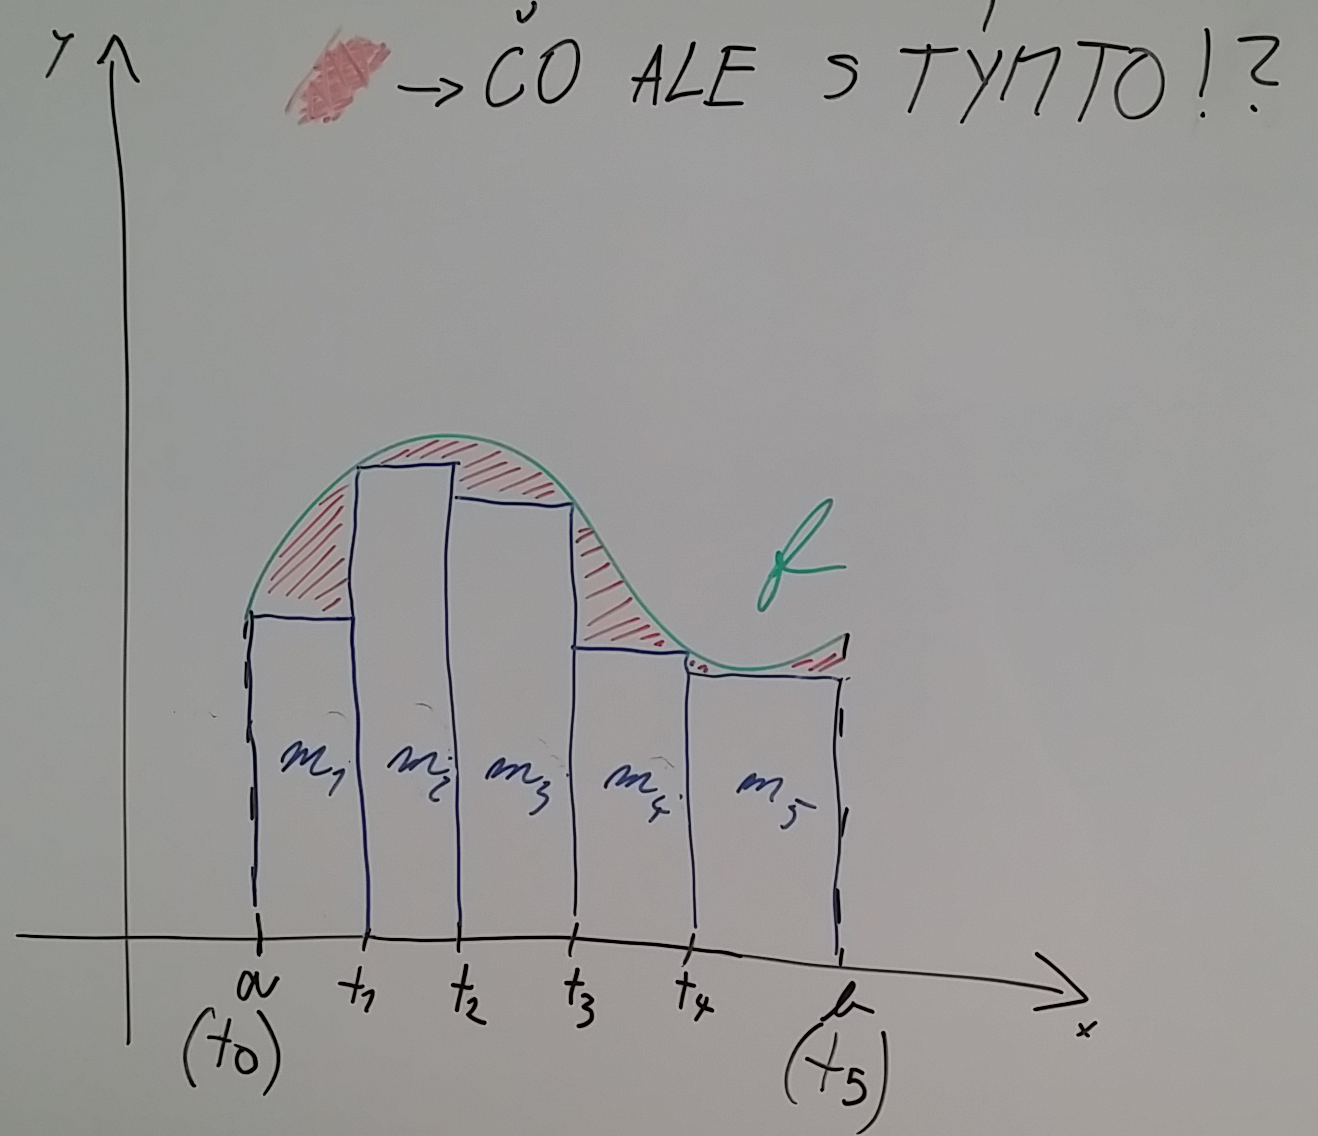
\includegraphics[scale=0.25]{img/int2}
	\end{center}
	\caption{Naznačenie obdĺžnikov pre dolný integrálny súčet\label{int2}}
\end{figure}

Otázne je ako vypočítať výšky obdĺžnikov. Ako výšku obdĺžnika budeme brať infimum funkcie $f$ obmedzenej na daný podinterval $[t_{i-1}, t_{i}]$. Takže platí $$m_{i}=inf\{ f(x)|x\in [t_{i-1}, t_{i}]\}$$ Pre potreby zápisu zadefinujeme \textbf{delenie} $P$ pričom bude platiť $$P: a=t_{0}<t_{1}<\dots <t_{n}<t_{n+1}=b$$

\begin{definition}
	Definujeme \textbf{dolný integrálny súčet} ako $L(f, P)=\sum_{i=1}^{n+1}m_{i(t_{i}, t_{i-1})}$
\end{definition}

\paragraph{}
Podobnými úvahami možeme prísť k hornému integrálnemu súčtu. (Pozri obrázok \ref{int3}). Výška obdĺžnikov pri hornom integrálnom súčte je zadefinovaná ako $$M_{i}=sup\{ f(x)|x\in [t_{i-1}, t_{i}]\}$$

\begin{figure}[H]
	\begin{center}
		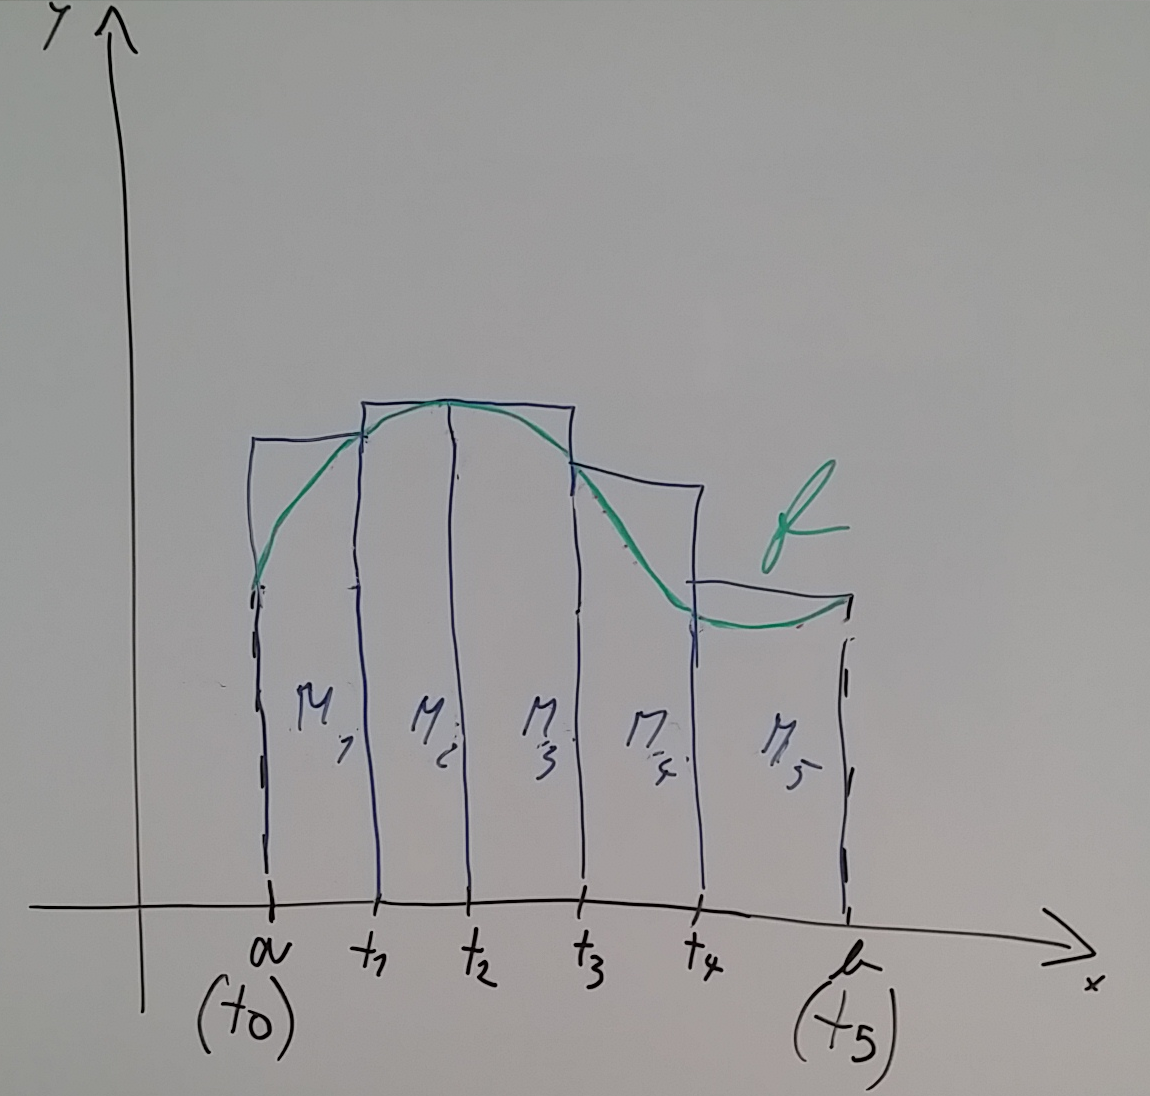
\includegraphics[scale=0.2]{img/int3}
	\end{center}
	\caption{Naznačenie obdĺžnikov pre horný integrálny súčet\label{int3}}
\end{figure}

\begin{definition}
	Potom zadefinujeme \textbf{holný integrálny súčet} ako $U(f, P)=\sum_{i=1}^{n+1}M_{i(t_{i}, t_{i-1})}$
\end{definition}

\paragraph{}
Jednoznačne platí že $L(f, P)\leq U(f, P)$. Teraz máme k dispozícii všetko potrebné aby sme zadefinovali horný a dolný integrál.

\begin{definition}
	$L\int_{a}^{b}f$ nazveme \textbf{dolný integrál} pričom platí že: $$L\int_{a}^{b}f= sup\{ L(f, P)|P\dots je \;delenie \;[a, b]\}$$
\end{definition}

\begin{definition}
	$U\int_{a}^{b}f$ nazveme \textbf{horný integrál} pričom platí že: $$U\int_{a}^{b}f= inf\{ U(f, P)|P\dots je \;delenie \;[a, b]\}$$
\end{definition}

\vspace{2cm}
\begin{center}
	\begin{Huge}
		\textbf{NASLEDUJE DEFINÍCIA \\ \vspace{1cm} INTEGRÁLU KONEČNE !!!!}
	\end{Huge}
\end{center}
\newpage

\begin{definition}
	Funkcia $f$ je integrovatelná na $[a, b]$ ak $L\int_{a}^{b}f=U\int_{a}^{b}f$, potom číslo $\int_{a}^{b}f=L\int_{a}^{b}f=U\int_{a}^{b}f$ sa nazýva \textbf{integrál funkcie} $f$ na intervale $[a, b]$.
\end{definition}

\paragraph{}
Otázne je ako zvoliť delenie $P$ ... pretože musí byť dostatočne jemné na to aby platil vzťah z definície. Pre zavádzame \textbf{zjemnené delenie} $Q$ pre ktoé platí, že $P\subset Q$ (Pozri obrázok \ref{int4})

\begin{figure}[H]
	\begin{center}
		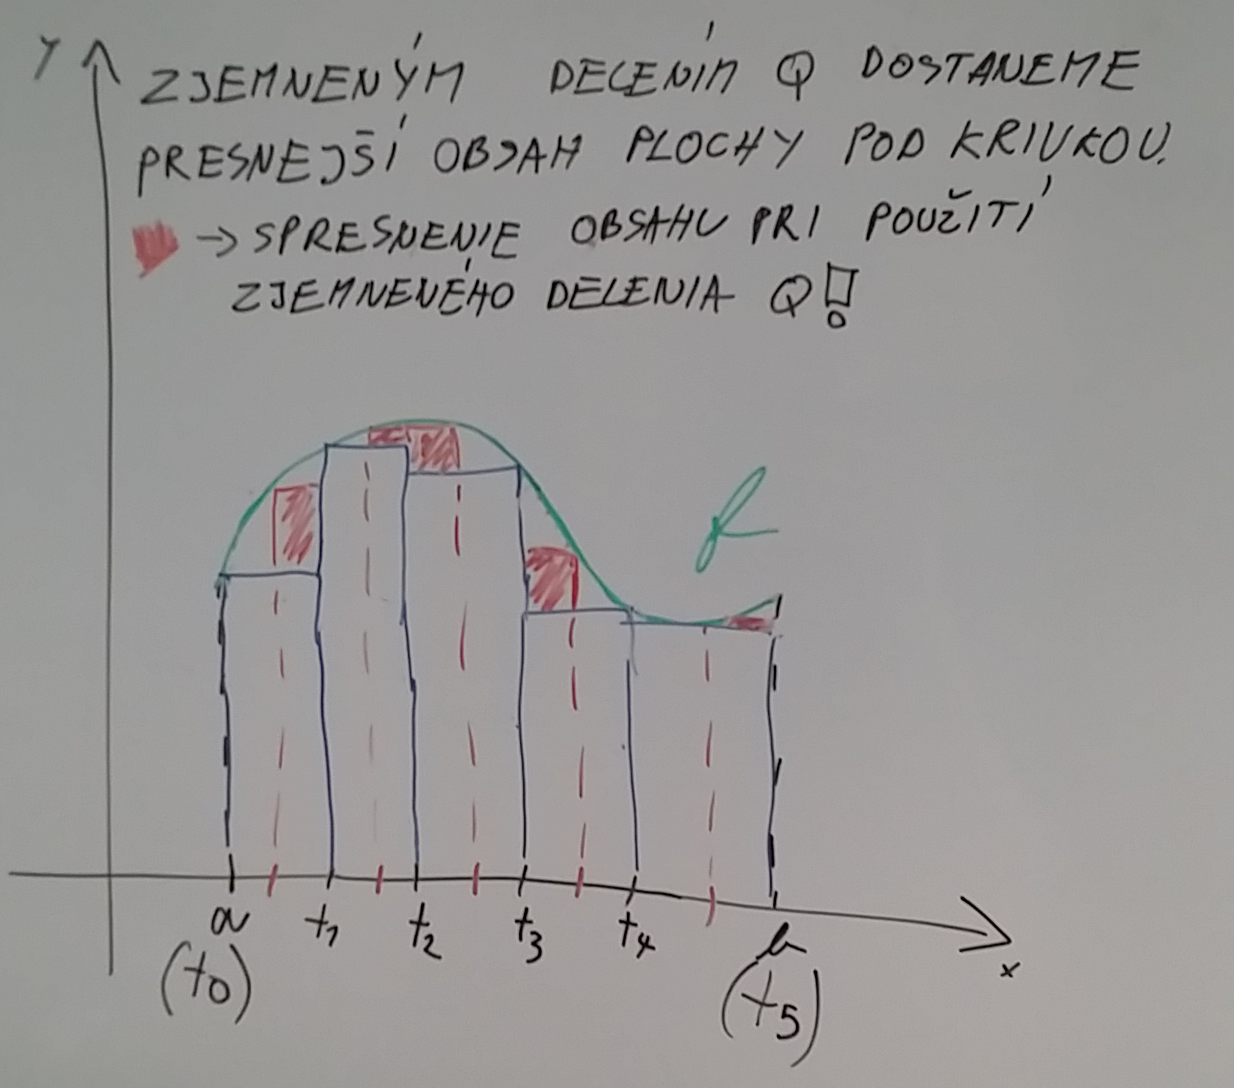
\includegraphics[scale=0.2]{img/int4}
	\end{center}
	\caption{Zjemnené delenie $Q$\label{int4}}
\end{figure}

\begin{sentence}
	Funkcia $f$ je integrovatelná na intervale $[a, b]$ práve vtedy, keď pre každé číslo $\epsilon >0$ exituje delenie $P$ (Ide iba o značenie ... úlaha je nájsť dostatočne jemné delenie) tak, že $U(f, P)-L(f, P)< \epsilon$.
\end{sentence}

%---------------------------------------------------------------------------------------------------------
% --------------------------------------------- pátý odstavec ---------------------------------------------
% ---------------------------------------------------------------------------------------------------------
\newpage
\textbf{Kombinatorika: pravidlo součtu a součinu, permutace, variace, kombinace, binomická věta, princip inkluze a
exkluze. Popisná statistika: číselné charakteristiky výběrů a grafické metody.}

\section{Kombinatorika}
\subsection{Pravidlo součtu a součinu}
\subsubsection{Pravidlo součtu}
\begin{definition}
	Lze-li úkol A provést m-způsoby a lze-li úkol B provést n-způsoby,
přičemž žádný z m-způsobů provedení úkolu A není totožný s žádným z n-způsobů
provedení úkolu B, pak provést úkol A nebo úkol B lze provést m + n způsoby.
\end{definition}

\subsubsection{Pravidlo součinu}
\begin{definition}
	Lze-li úkol C rozložit na po sobě následující úkoly A a B (tj. provést
C znamená provést nejdřív A a potom B) a lze-li úkol A provést m způsoby a úkol B lze
provést n způsoby, pak lze úkol C provést $m \cdot n $ způsoby.	
\end{definition}

\subsection{Variace}
\subsubsection{bez opakování}
\begin{definition}
	Je dáno n (navzájem různých) objektů a číslo $r \leq n$. Variace r
(objektů) z n (objektů) je libovolný výběr r objektů z daných n objektů, ve kterém záleží na
pořadí vybíraných objektů. Počet takových variací značíme V(n, r).
\end{definition}
\begin{sentence}
	$V(n, r) = n \cdot (n - 1) \cdot \dots \cdot (n - r + 1)$
\end{sentence}
\paragraph{Poznámka.} $V(n, r) = \frac{n!}{(n - r)!} = \frac{n \cdot (n - 1) \cdot \dots \cdot (n - r + 1) \cdot (n - r) \cdot \dots \cdot 1}{(n - r) \cdot \dots \cdot 1} = n \cdot (n - 1) \cdot \dots \cdot (n - r + 1)$

\subsubsection{s opakováním}
\begin{definition}
	Jsou dány objekty n různých typů. Objektů každého typu je neomezeně mnoho a jsou navzájem nerozlišitelné. Variace r (objektů) z n (objektů) s opakováním je libovolný výběr r objektů z daných objektů n typů, ve kterém záleží na pořadí vybíraných objektů. Počet takových variací značíme $\overline{V}(n, r)$.	
\end{definition}
\begin{sentence}
	$\overline{V}(n, r) = n^r$.
\end{sentence}

\subsection{Permutace}
\subsection{bez opakování}
\begin{definition}
	Permutace n (navzájem různých) objektů je libovolné seřazení těchto objektů, tj. seřazení od prvního k n-tému. Počet permutací n objektů budeme značit P(n).
\end{definition}
\begin{sentence}
	$P(n) = V(n, n) = n!$
\end{sentence}

\subsection{s opakováním}
\begin{definition}
	Je dáno n objektů rozdělených do r skupin, které mají po řadě $n_1, \dots,n_r$ objektů, tj. $n_1 + \dots + n_r = n$. Objekty v každé ze skupin jsou navzájem nerozlišitelné. Každé seřazení těchto n objektů se nazývá permutace s opakováním (daným parametry ($n_1, \dots, n_r$)). Počet takových permutací značíme P($n_1, \dots, n_r$).
\end{definition}
\begin{sentence}
	Pro $n_1 + \dots + n_r = n$ je P($n_1, \dots, n_r$)$ = \frac{n!}{n_1! \cdot \dots \cdot n_r!}$.
\end{sentence}

\subsection{Kombinace}
\subsubsection{bez opakování}
\begin{definition}
	Je dáno n (navzájem různých) objektů a číslo $r \leq n$. Kombinace r (objektů) z n (objektů) je libovolný výběr r objektů z daných n objektů, ve kterém nezáleží na pořadí vybíraných objektů. Počet takových kombinací značíme $n \choose r$ (nebo C(n, r)).
\end{definition}
\begin{sentence}
	${n \choose r} = \frac{n!}{(n - r)! \cdot r!}$
\end{sentence}
$$ {n \choose r} = {n \choose n - r} $$
$${n \choose n} = 1 \text{ a } {n \choose 0} = 1 $$
\paragraph{Poznámka.} ${n \choose k} = {n - 1 \choose k - 1} + {n - 1 \choose k}$.

\subsubsection{s opakováním}
\begin{definition}
	Jsou dány objekty n různých typů. Objektů každého typu je neomezeně mnoho a jsou navzájem nerozlišitelné. Kombinace r (objektů) z n (objektů) s opakováním je libovolný výběr r objektů z daných objektů n typů, ve kterém nezáleží na pořadí vybíraných objektů. Počet takových kombinací značíme $\overline{C}(n, r)$.
\end{definition}
\begin{sentence}
	$\overline{C}(n, r) = {n + r - 1 \choose n - 1}$.
\end{sentence}

\subsection{Binomická věta}
\begin{sentence}
Pro reálné číslo $x$ a nezáporné celé $n$ je $$(1 + x)^n = \sum\limits_{k=0}^n {n \choose k} x^k $$
\end{sentence}

\subsection{Princip inkluze a exkluze}
\begin{sentence}
	Pro množiny $A_1, \dots, A_n$ platí $$|A_1 \cup A_2 \cup \dots \cup A_n| = \sum\limits_{\emptyset \neq I \subseteq \{1, 2, \dots , n \}} (-1)^{|I| + 1} |\bigcap_{i \in I} A_i |$$
\end{sentence}
\begin{example}
	V nabídce volitelných předmětů je němčina a angličtina. Němčinu si zvolilo 15, angličtinu 30 a oba jazyky 5 studentů. Kolik studentů si jako volitelný předmět vybralo cizí jazyk (tj. NJ + AJ)? Označme N a A po řadě množiny studentů, kteří si zapsali NJ a AJ. Sečteme-li $|N|$ (počet co si zapsali němčinu) a $|A|$ (počet co si zapsali angličtinu), počítáme dvakrát ty, kteří si zapsali NJ a AJ (těch je $|N \cap A|$. Ty tedy musíme od $|N| + |A|$ odečíst. Počet $|N \cup A|$ těch, kteří si zapsali NJ nebo AJ tedy $$|N \cup A| = |N| + |A| - |N \cap A| = 15 + 30 - 5 = 40$$
\end{example}
\paragraph{Poznámka.} $|A_1 \cup A_2 \cup A_3| = |A_1| + |A_2| + |A_3| - |A_1 \cap A_2| - |A_1 \cap A_3| - |A_2 \cap A_3| + |A_1 \cap A_2 \cap A_3|$

\section{Popisná statistika}
\subsection{Číselné charakteristiky výběrů}
\subsubsection{Výběrový (aritmetický) průměr}
\begin{center}
	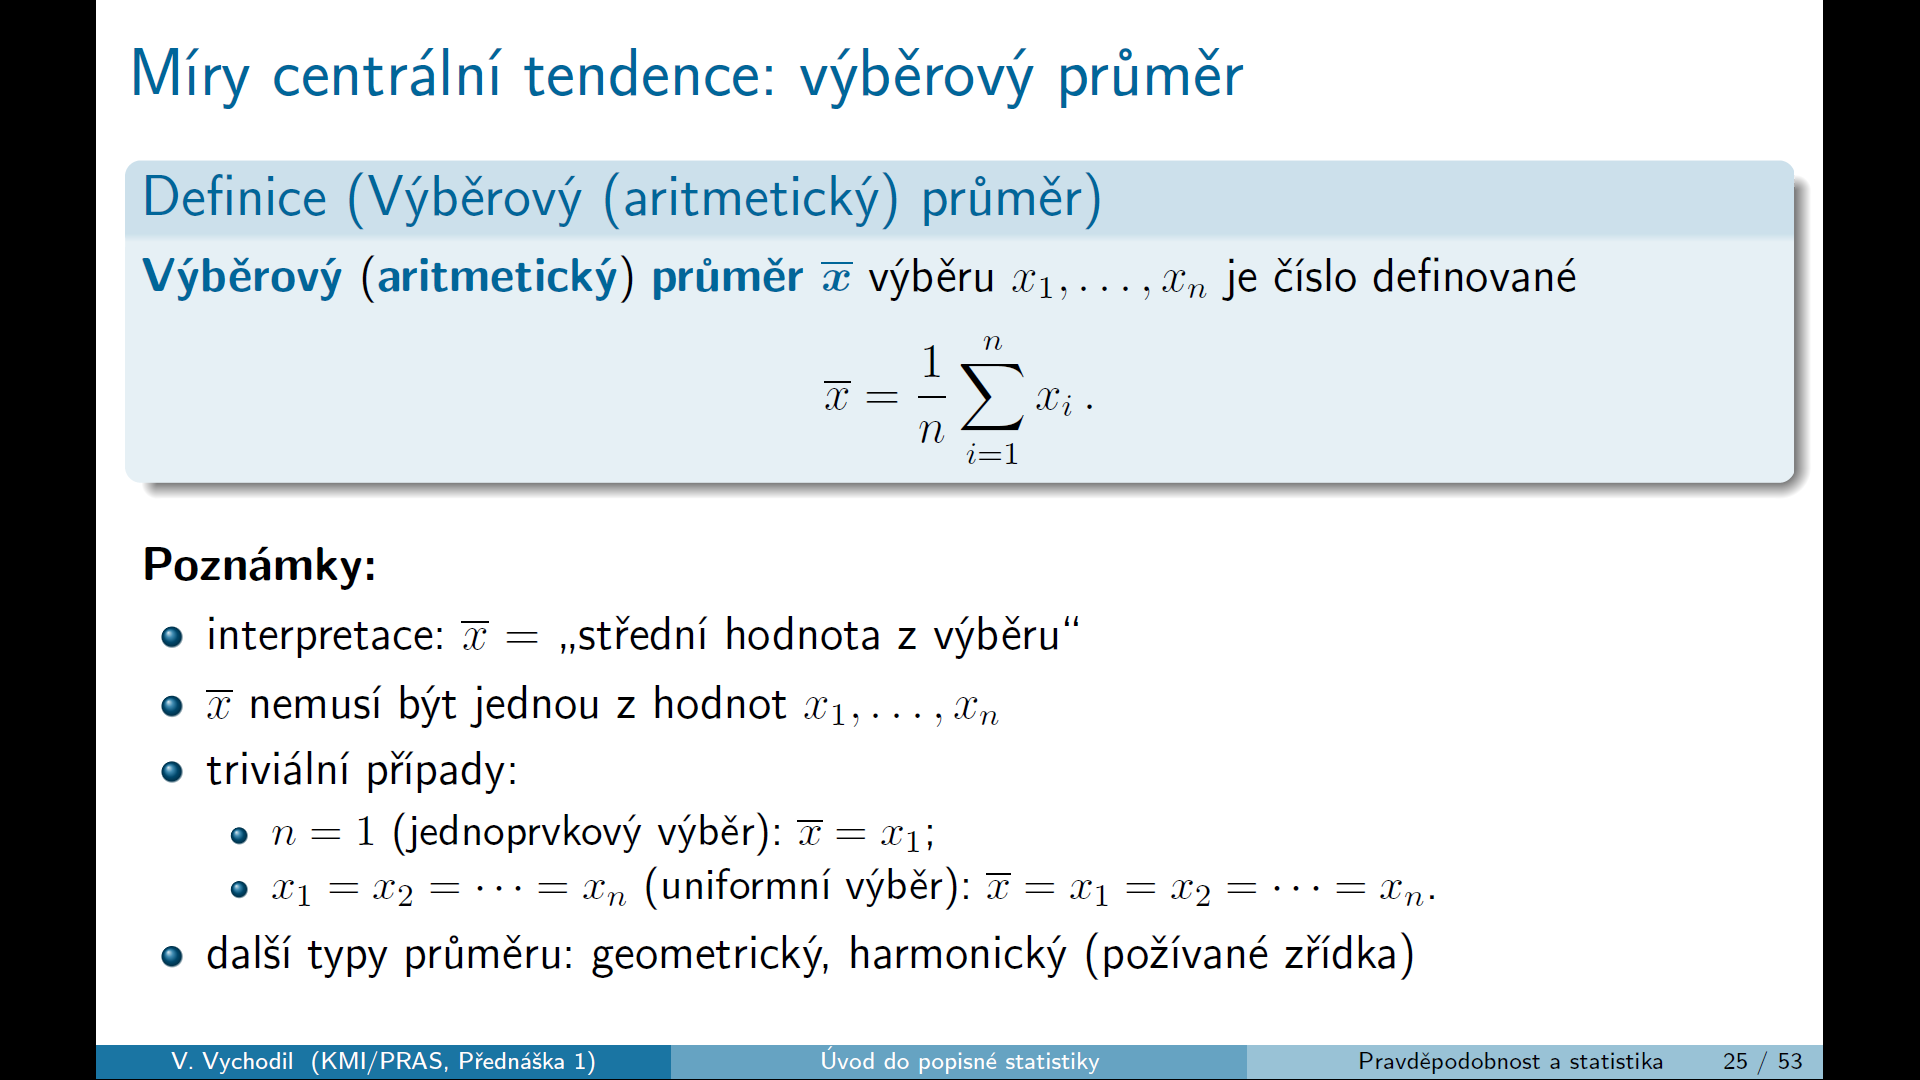
\includegraphics[scale=0.32]{img/prumer_definition.png}
	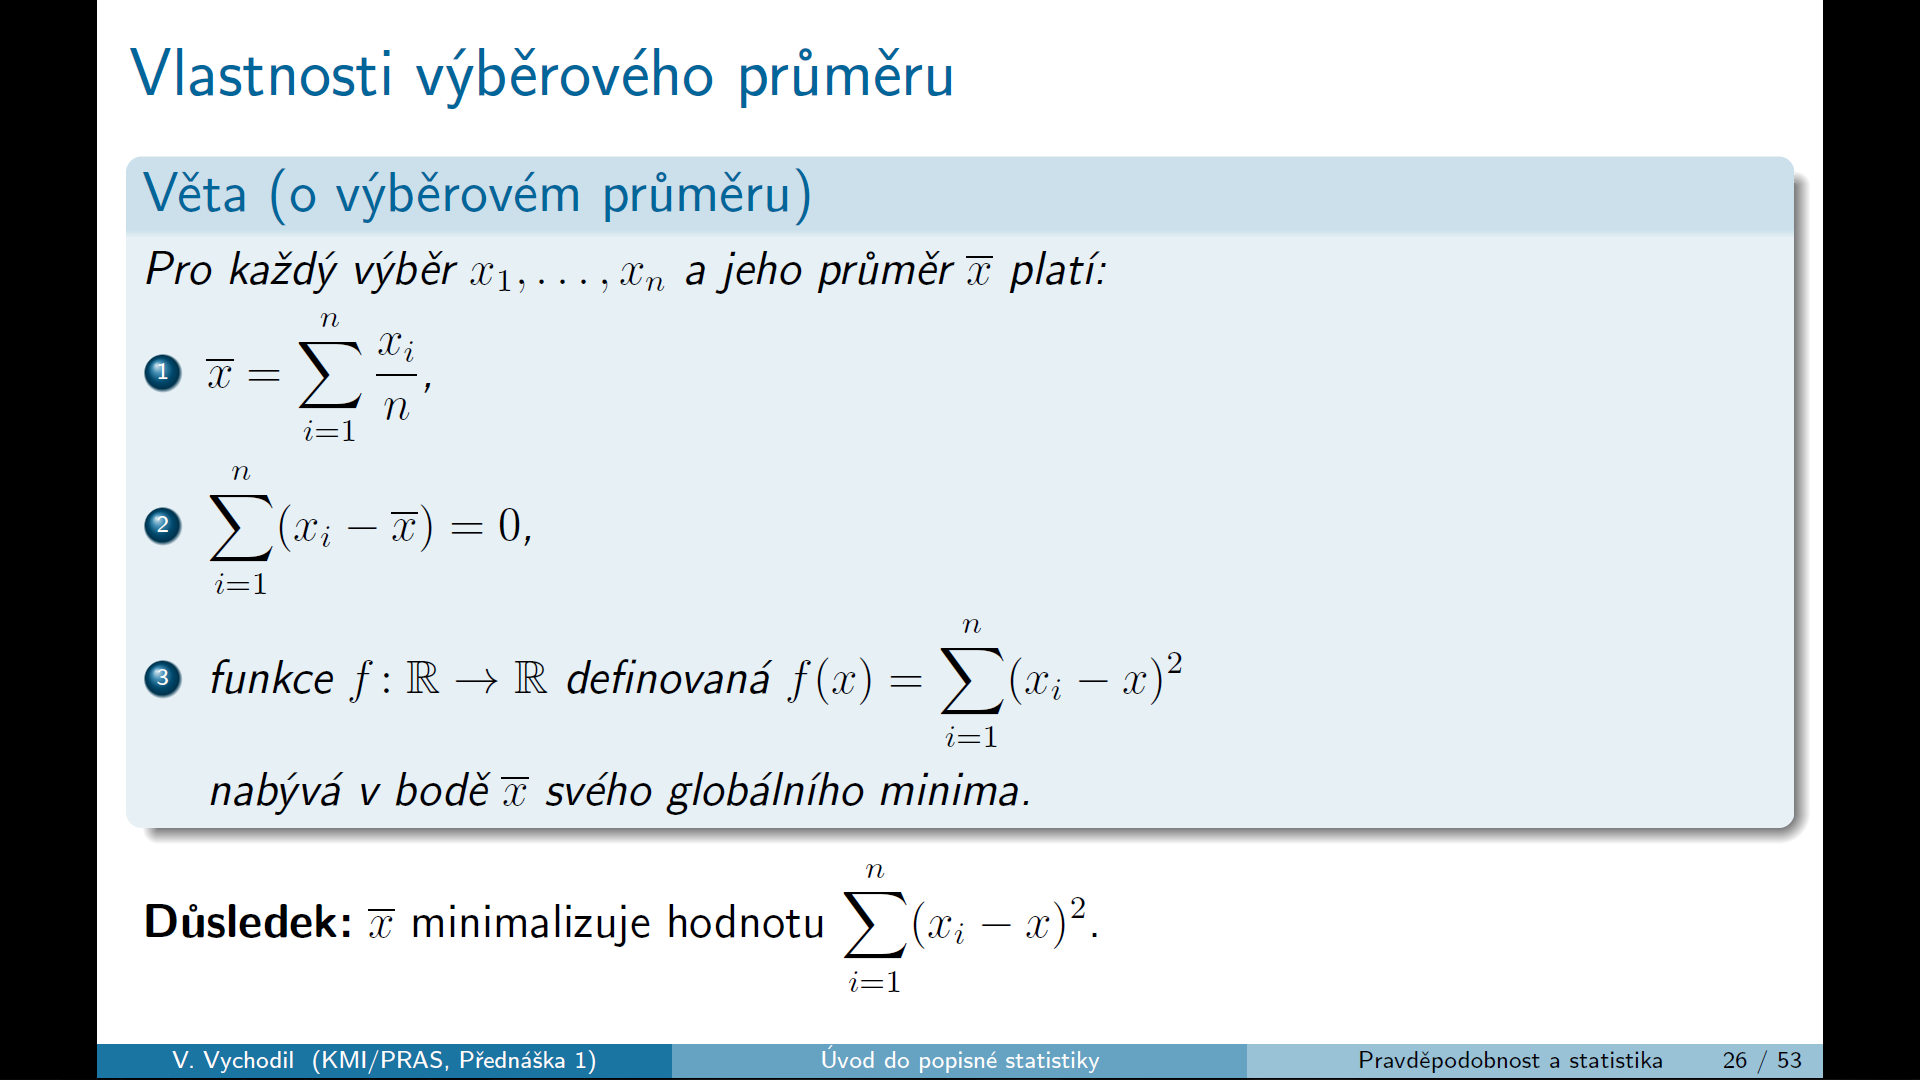
\includegraphics[scale=0.32]{img/prumer_properties.png}
\end{center}

\subsubsection{Výběrový rozptyl a Směrodatná odchylka}
\begin{center}
	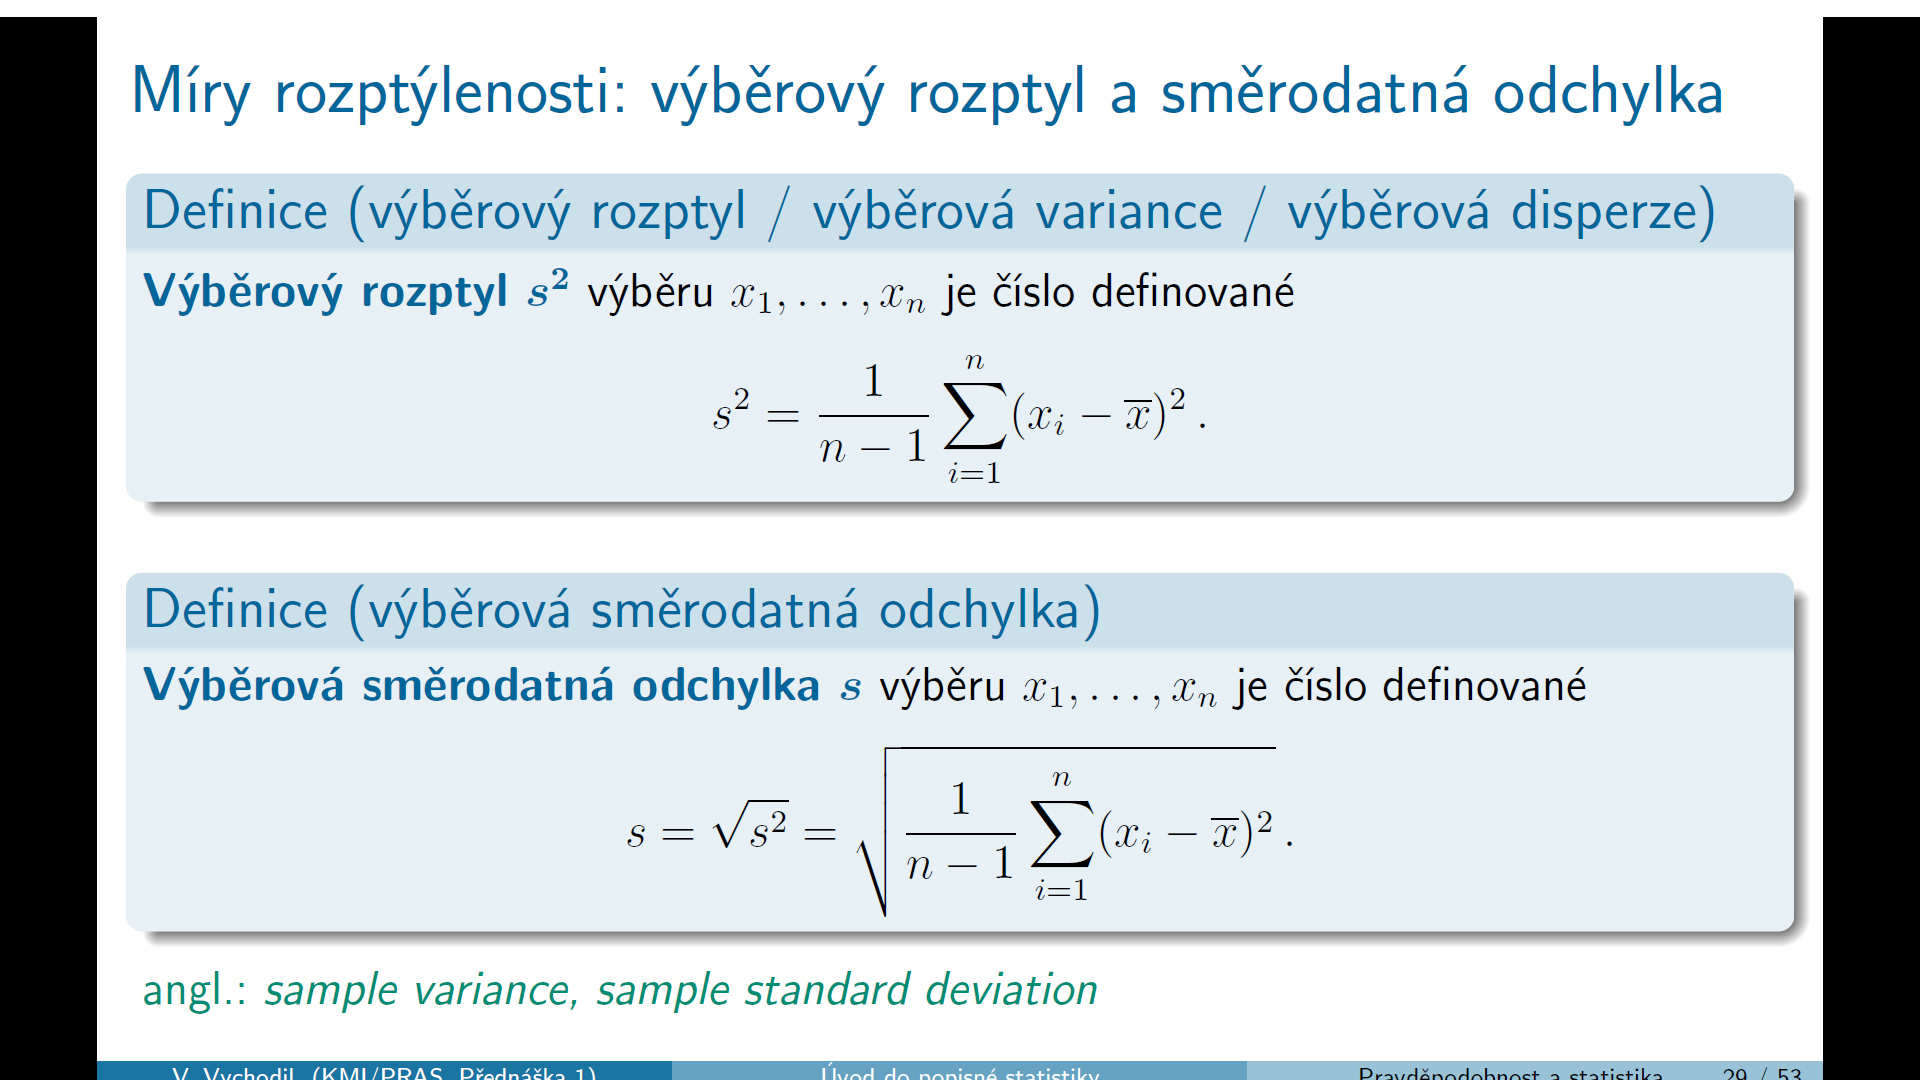
\includegraphics[scale=0.32]{img/rozptyl_odchylka}
	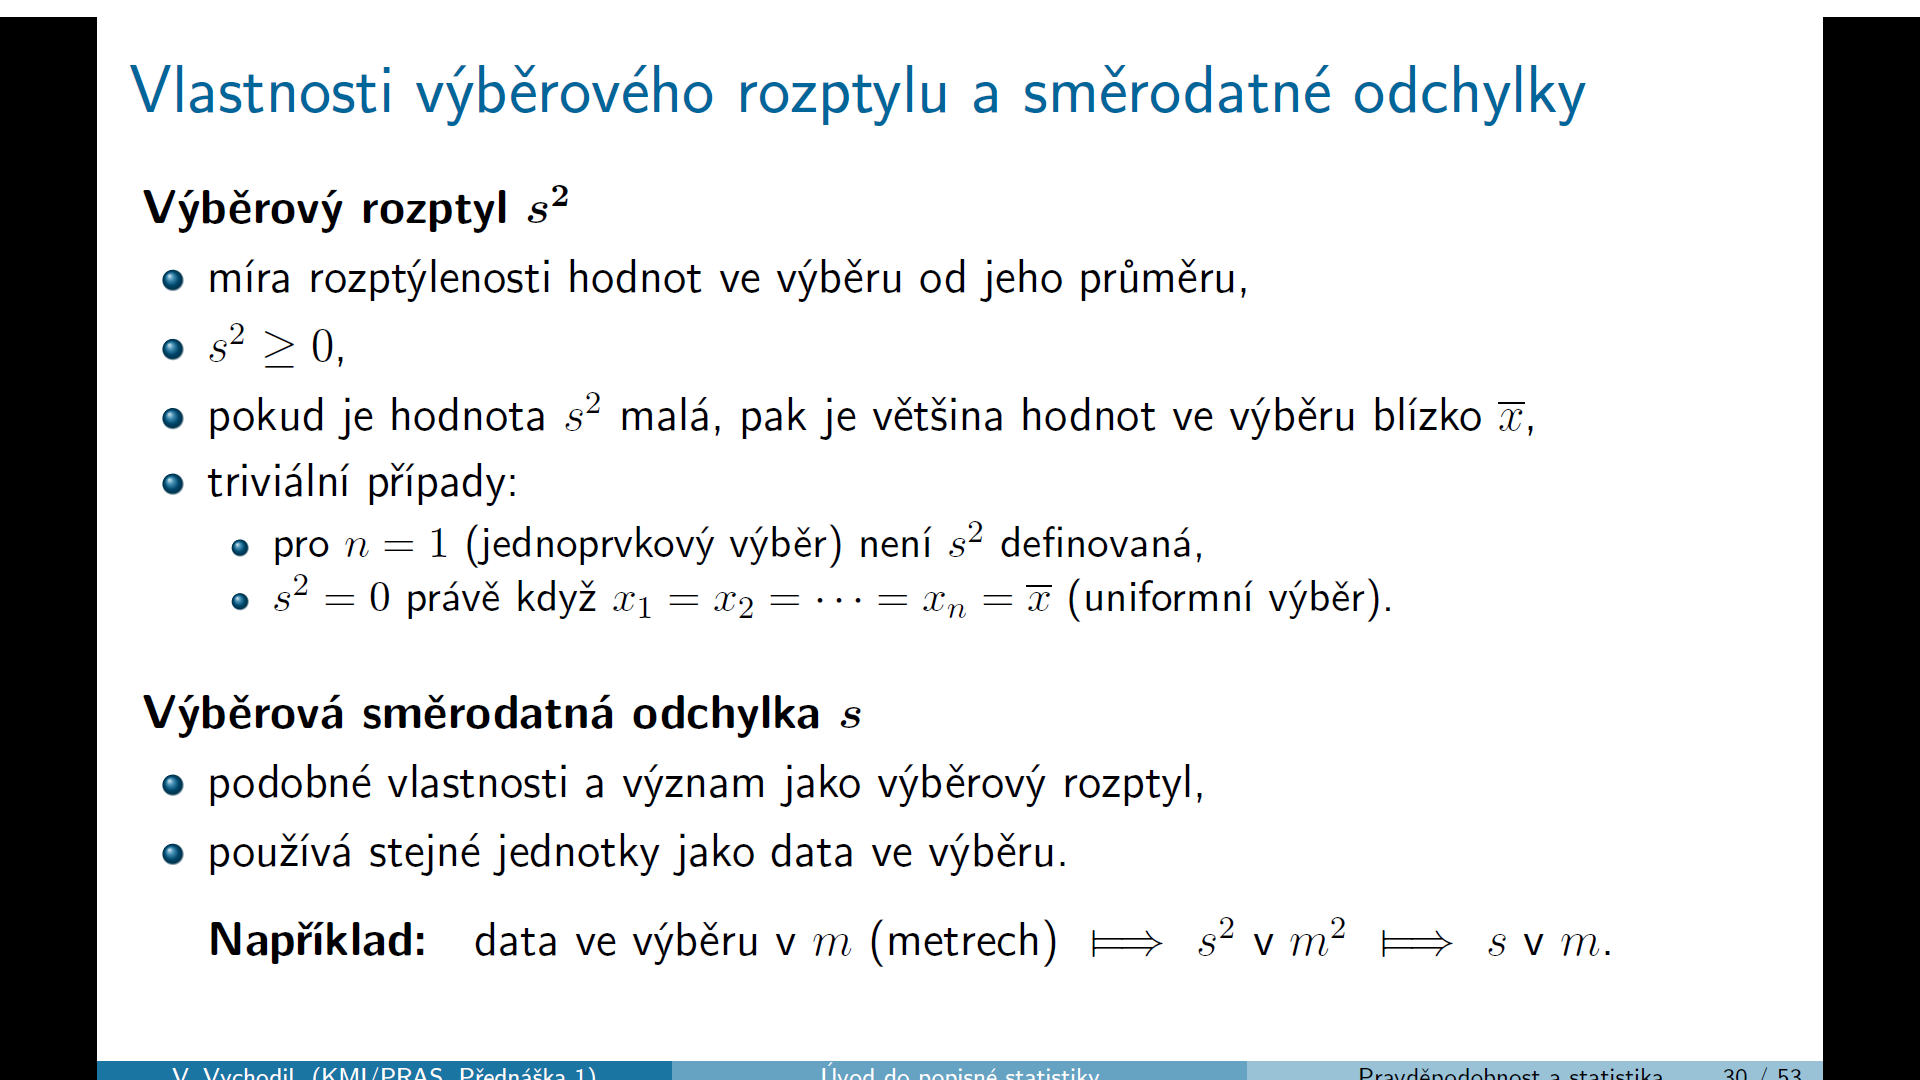
\includegraphics[scale=0.32]{img/rozptyl_odchylka_properties}
\end{center}
\newpage
\subsection{Grafické metody}
\begin{center}
	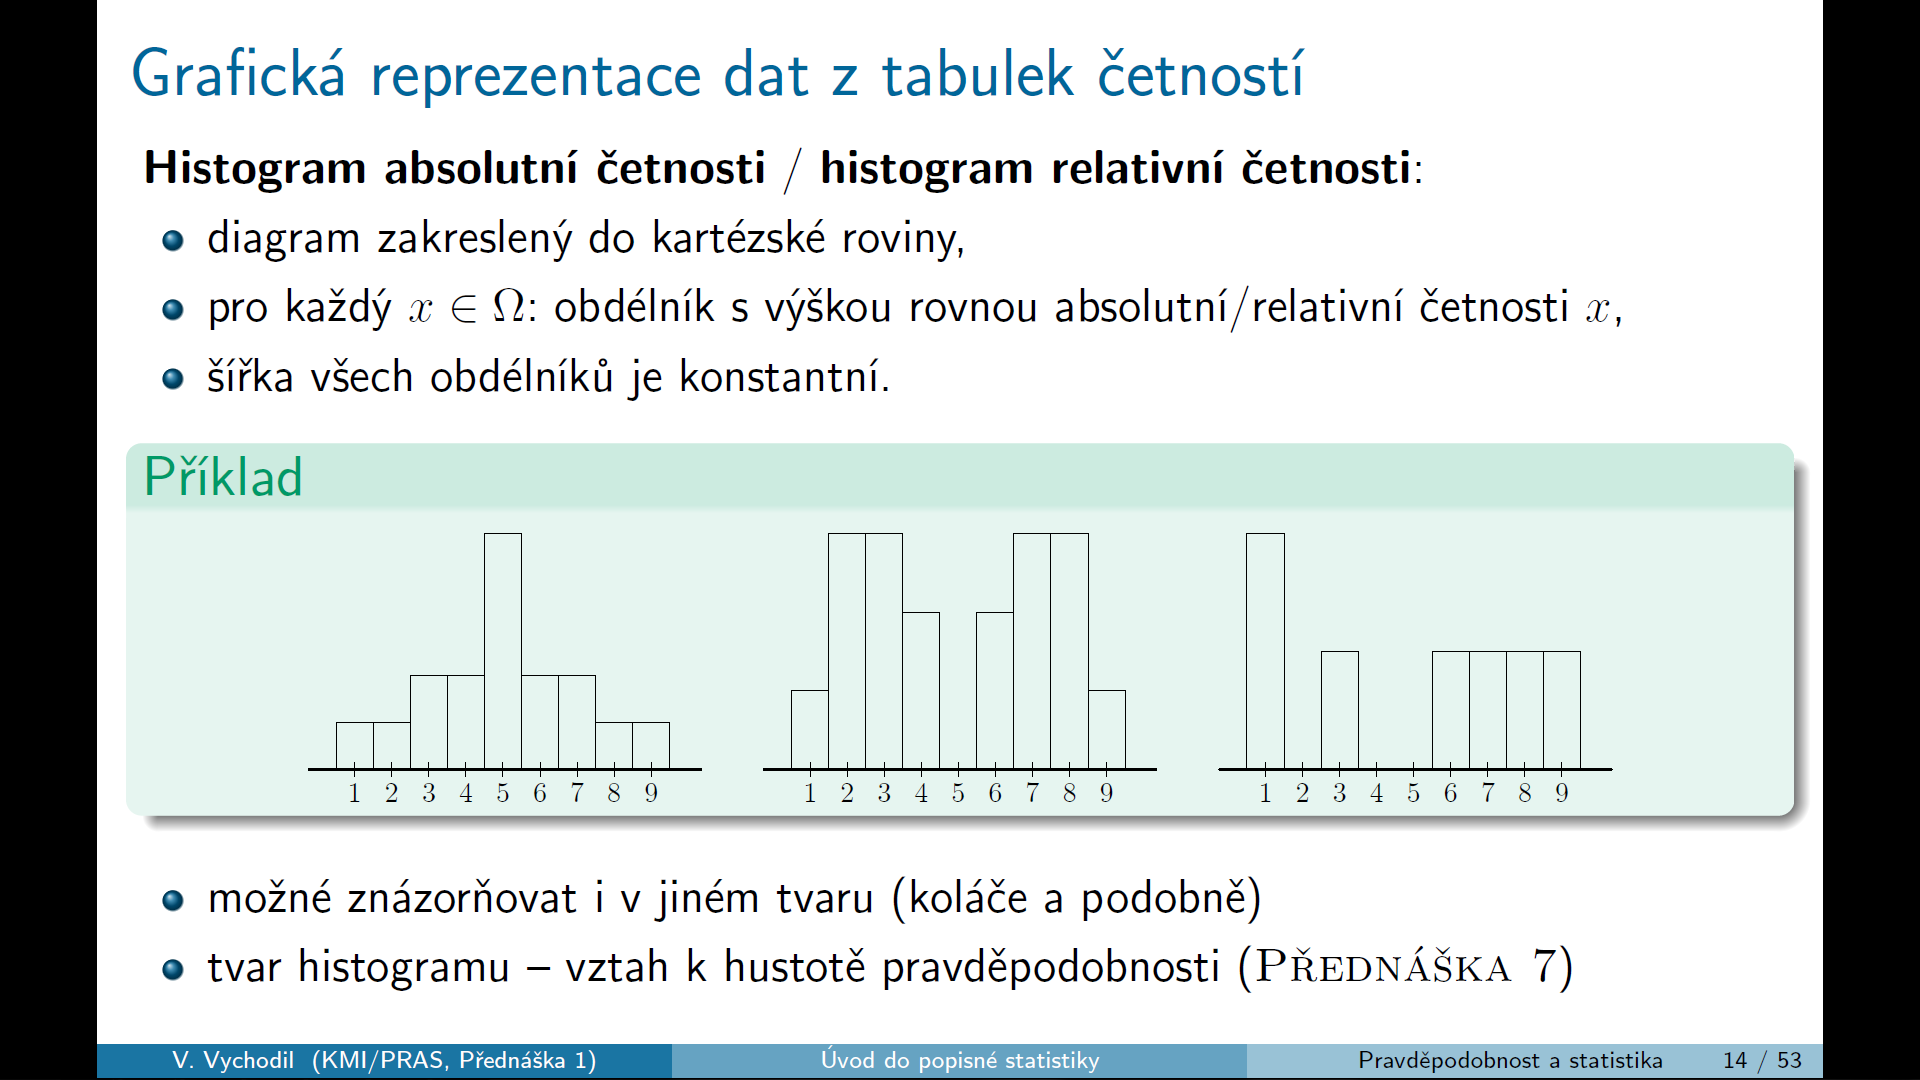
\includegraphics[scale=0.32]{img/graficke_metody_histogram}
	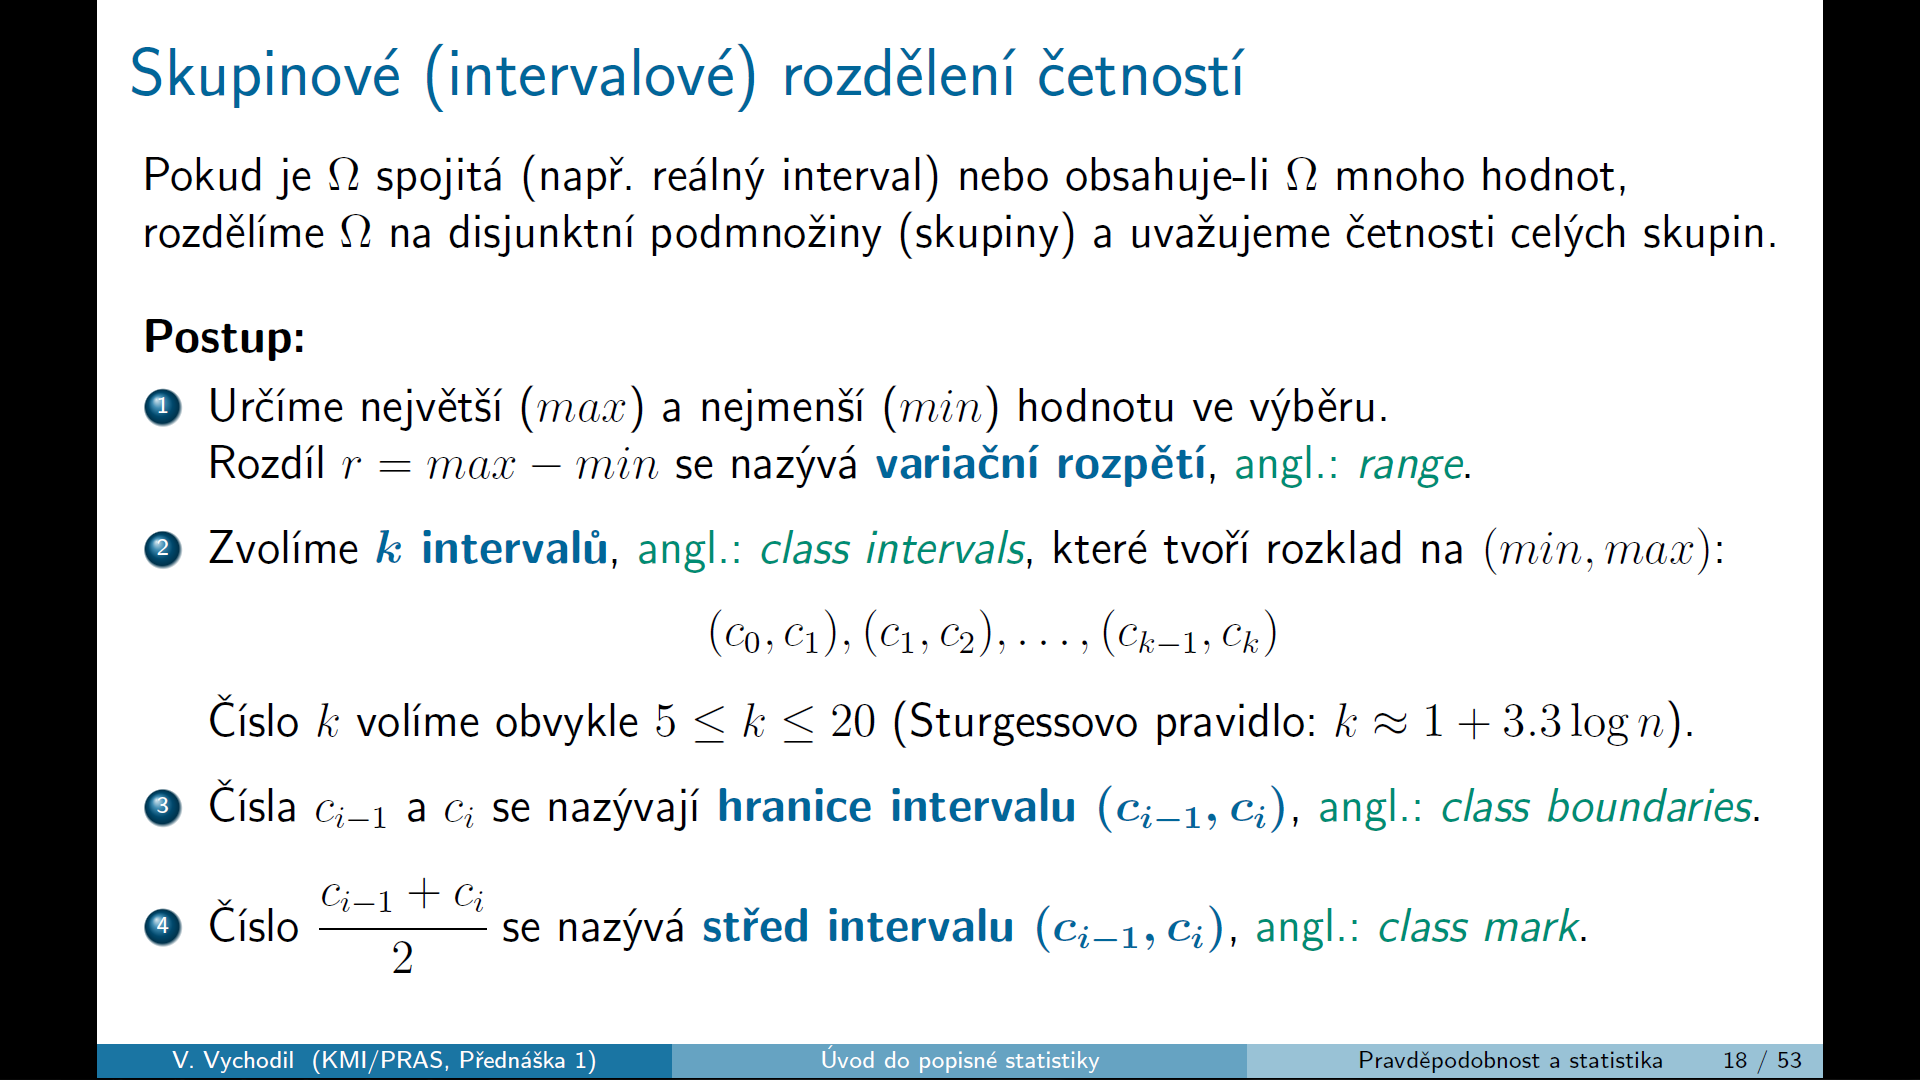
\includegraphics[scale=0.32]{img/graficke_metody_intervalove_rozdeleni}
	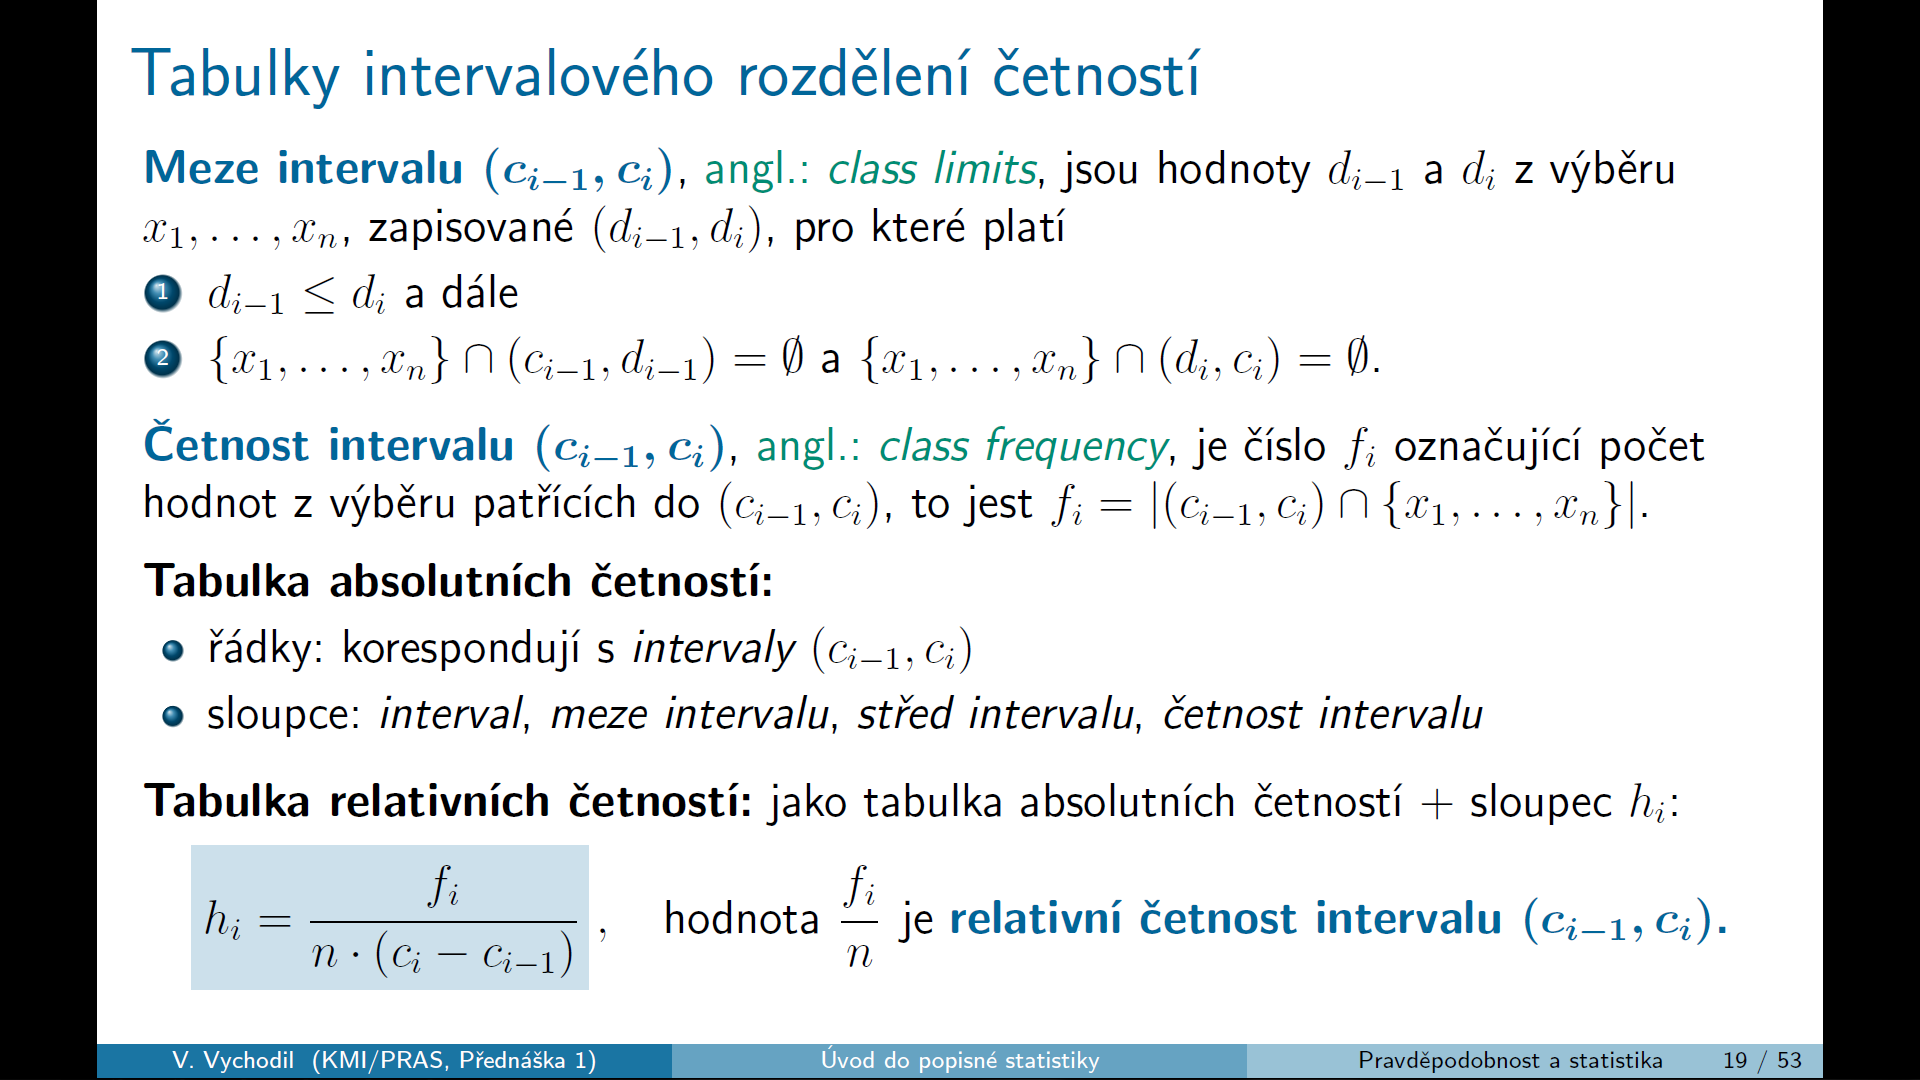
\includegraphics[scale=0.32]{img/graficke_metody_intervalove_rozdeleni_tabulky}
	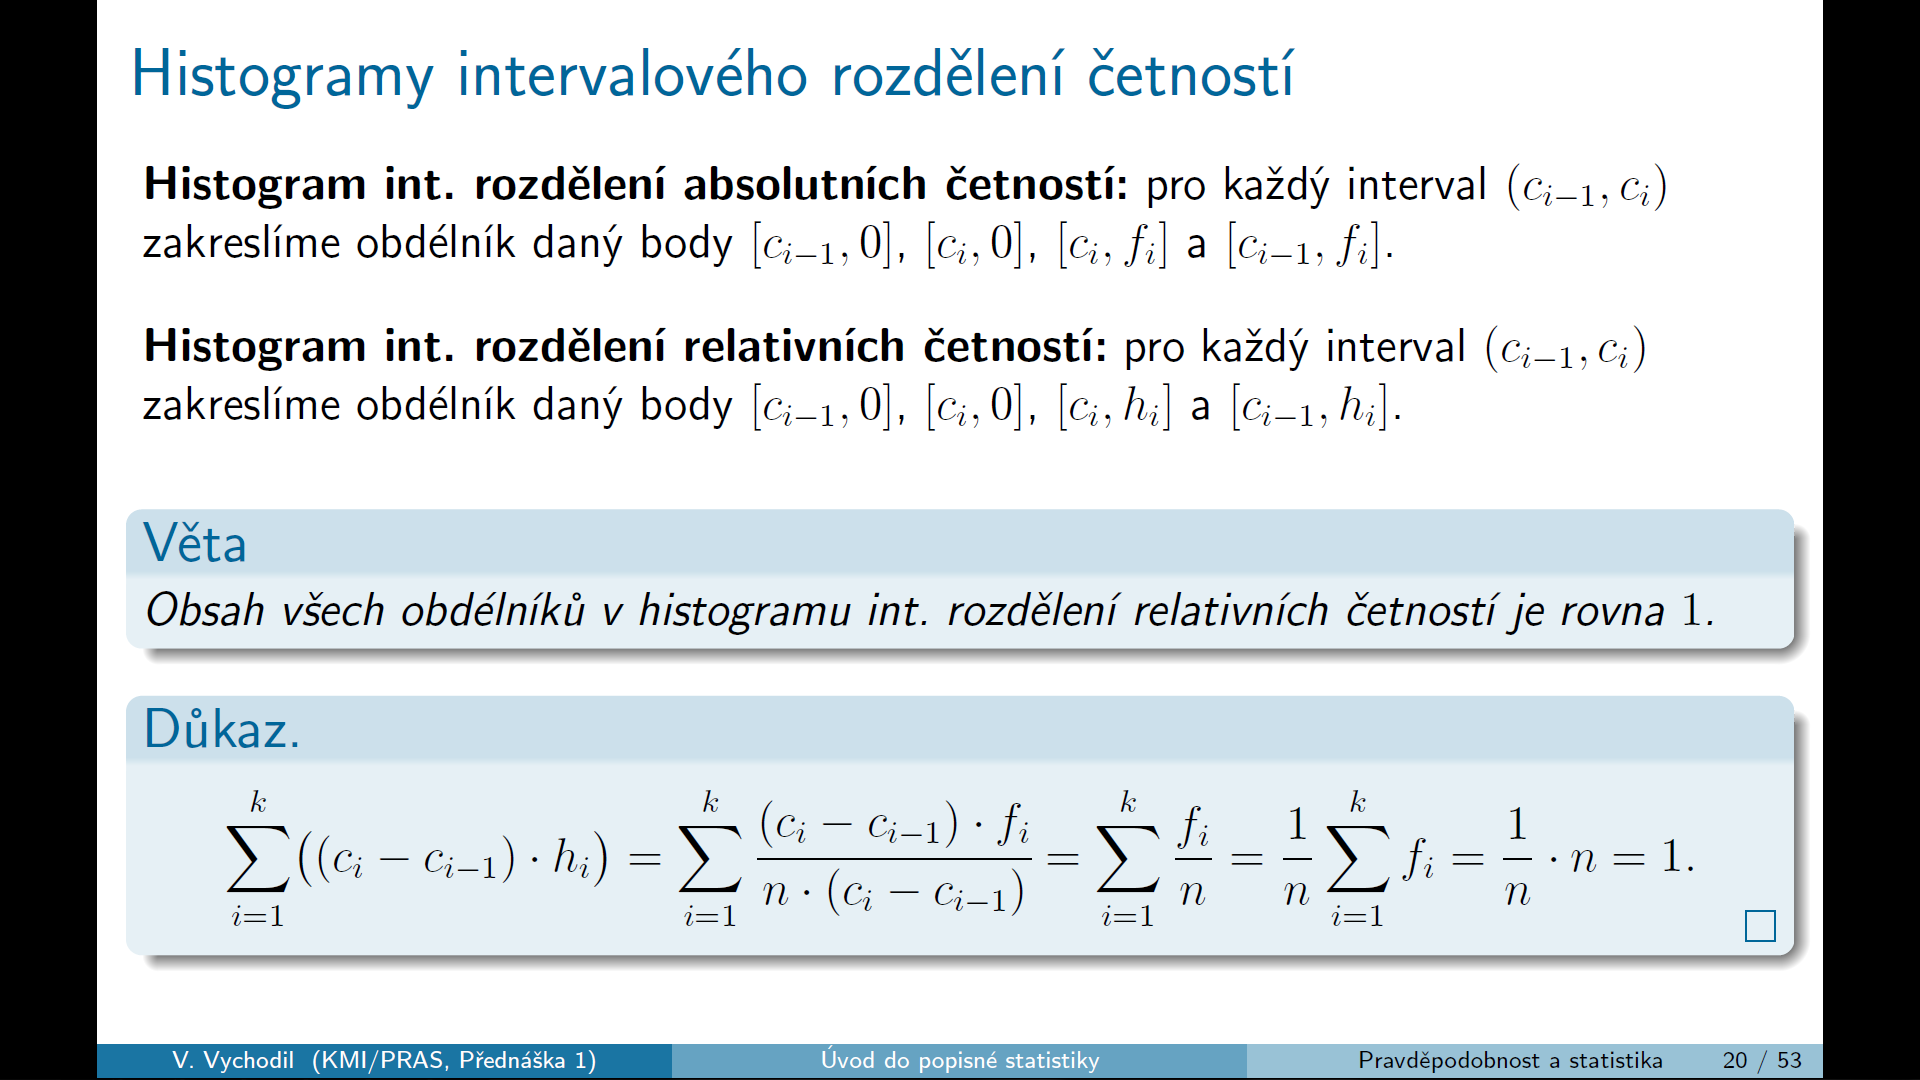
\includegraphics[scale=0.32]{img/graficke_metody_intervalove_rozdeleni_histogramy}
\end{center}
\paragraph{Poznámka.} Další metody jsou např.: sloupcový graf, koláčový graf nebo bodový graf (myslím, že k tomu není třeba nic psát)

% ---------------------------------------------------------------------------------------------------------
% --------------------------------------------- šestý odstavec ---------------------------------------------
% ---------------------------------------------------------------------------------------------------------
\newpage
\textbf{Náhodné jevy, pravděpodobnostní míra. Podmíněná pravděpodobnost, nezávislost jevů. Náhodná veličina, distribuční
funkce. Příklady rozdělení diskrétních a spojitých náhodných veličin. Náhodné vektory: sdružené a
marginální rozdělení. Bodové odhady. Základy testování hypotéz.}

\section{Pravděpodobnost}
\subsection{Náhodné jevy}
\begin{center}
	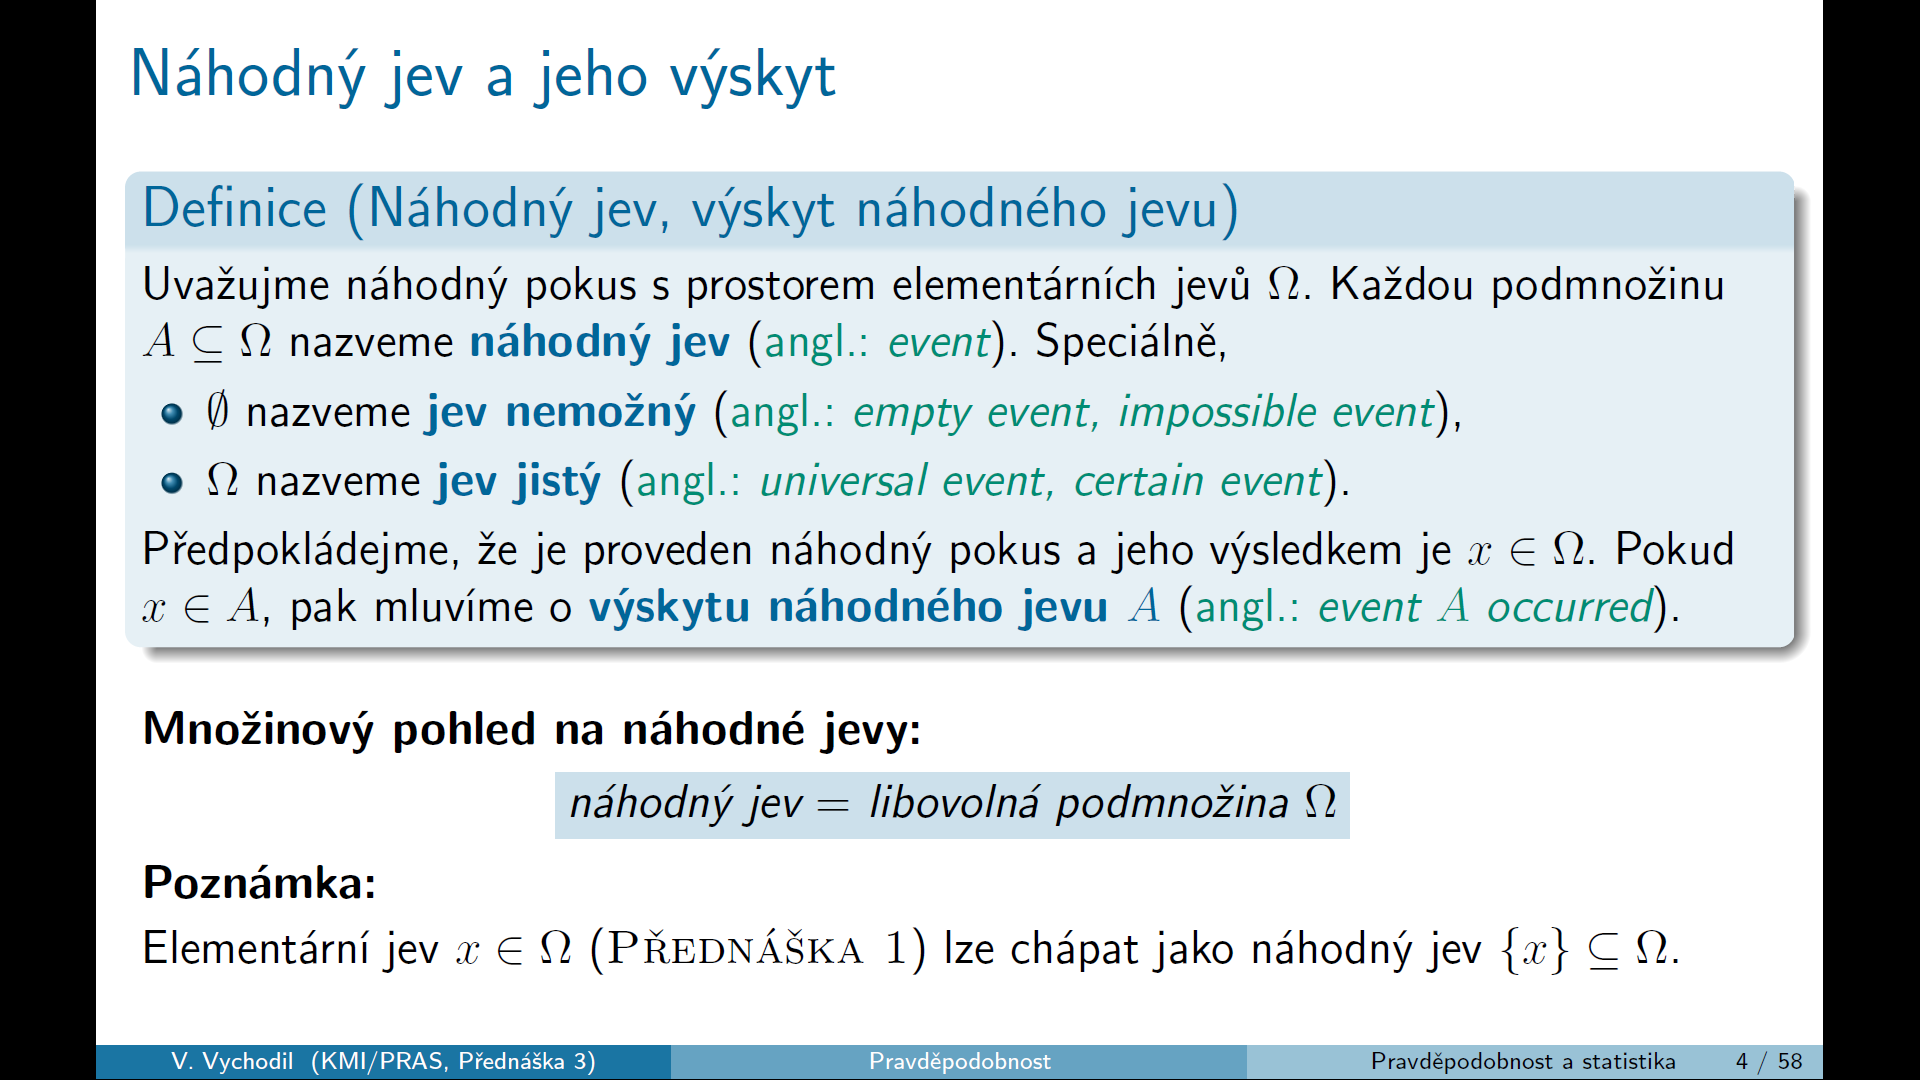
\includegraphics[scale=0.32]{img/nahodny_jev}
	\includegraphics[scale=0.32]{img/nahodny_jev_vztahy}
	\includegraphics[scale=0.32]{img/nahodny_jev_operace}
\end{center}
\newpage
\subsection{Pravděpodobnostní míra}
\begin{center}
	\includegraphics[scale=0.32]{img/pravdepod_mira}
\end{center}

\subsection{Podmíněná pravděpodobnost}
\begin{center}
	\includegraphics[scale=0.32]{img/podminena_pravdepod}
	\includegraphics[scale=0.32]{img/podminena_pravdepod_properties}
\end{center}

\subsection{Nezávislost jevů}
\begin{center}
	\includegraphics[scale=0.32]{img/nezavisle_nahod_jevy}
	\includegraphics[scale=0.32]{img/nezavisle_nahod_jevy_properties}
	\includegraphics[scale=0.32]{img/nezavisle_nahod_jevy_trivialni}
\end{center}
\newpage
\subsection{Náhodná veličina}
\begin{center}
	\includegraphics[scale=0.32]{img/nahod_velicina}
\end{center}

\subsection{Distribuční funkce}
\begin{center}
	\includegraphics[scale=0.32]{img/distribucni_fce}
\end{center}

\subsection{Rozdělení diskrétních náhodných veličin}
\subsubsection{Alternativní rozdělení}
\begin{center}
	\includegraphics[scale=0.32]{img/diskretni_rozdeleni_alternativni}
\end{center}
\newpage
\subsubsection{Binomické rozdělení}
\begin{center}
	\includegraphics[scale=0.32]{img/diskretni_rozdeleni_binomicke}
\end{center}
\paragraph{} Budeme uvažovat náhodný pokus, ve kterém určitý náhodný jev nastane s pravděpodobností $p$. Tento pokus opakujeme nezávisle $n$-krát a sledujeme výskyt sledovaného náhodného jevu v těchto $n$ nezávislých opakováních téhož náhodného pokusu, přičemž pravděpodobnost, že v každém jednotlivém opakování náhodného pokusu je sledovaný náhodný jev, je rovna $p$.
\paragraph{} Náhodná veličina X představující počet opakování daného náhodného pokusu z celkového počtu $n$ nezávislých opakování, ve kterých sledovaný náhodný jev nastane, má binomické rozdělení $b(n, p)$.
\paragraph{Poznámka.} Typickým příkladem je výběr prvku s vracením, vícenásobný hod kostkou.
\newpage
\subsubsection{Poissonovo rozdělení}
\begin{center}
	\includegraphics[scale=0.32]{img/diskretni_rozdeleni_poissonovo}
\end{center}
\paragraph{Poznámka.} Tímto rozdělením se řídí počet nějakých událostí během určitého časového intervalu. (Počet zákazníků za 1 hodinu, počet poruch za 100 hodin...)
\newpage
\subsubsection{Geometrické rozdělení}
\begin{center}
	\includegraphics[scale=0.32]{img/diskretni_rozdeleni_geometricke}
\end{center}
\paragraph{} Geometrickým rozdělením se řídí počet neúspěšných opakování náhodného pokusu předcházejících prvnímu úspěšnému opakování při nezávislých opakováních téhož náhodného pokusu, kde úspěšnost každého pokusu je $p$
\paragraph{} Počet pokusů nutných k dosažení 1. úspěchu je $x + 1$. $f_x(x)$ udává pravděpodobnost, že prvních x pokusů bude neúspěšných a $x + 1$ skončí úspěchem.
\newpage
\subsection{Rozdělení spojitých náhodných veličin}
\subsubsection{Rovnoměrné (uniformní) rozdělení}
\begin{center}
	\includegraphics[scale=0.30]{img/spojite_rozdeleni_uniformni}
	\includegraphics[scale=0.30]{img/spojite_rozdeleni_uniformni_priklad}
\end{center}
\paragraph{} Náhodné veličiny řídící se rovnoměrným rozdělením: \begin{itemize}
	\item chyba při zaokrouhlení čísla
	\item doba čekání na uskutečnění jevu, který se vyskytuje v pravidelných intervalech
\end{itemize}
\subsubsection{Normální rozdělení}
\begin{center}
	\includegraphics[scale=0.32]{img/spojite_rozdeleni_normalni}
\end{center}
\paragraph{} Normální rozdělení má zásadní význam v teorii pravděpodobnosti a v matematické statistice. Má význam tam kde je kolísání náhodné veličiny způsobeno součtem velkého počtu nepatrných vzájemně nezávislých vlivů.

\subsubsection{Exponenciální rozdělení}
\begin{center}
	\includegraphics[scale=0.32]{img/spojite_rozdeleni_exponencialni}
\end{center}
\paragraph{} Využívá se k popisu reálných dějů - životnost součástí strojů, dobu bezporuchové činnosti ...

\subsection{Náhodné vektory}
\subsubsection{Sdružené rozdělení}
\begin{center}
	\includegraphics[scale=0.32]{img/sdruzene_rozdeleni}
\end{center}
\subsubsection{Marginální rozdělení}
\begin{center}
	\includegraphics[scale=0.32]{img/marginalni_rozdeleni}
\end{center}

\section{Bodové odhady}
\begin{center}
	\includegraphics[scale=0.32]{img/bodove_odhady_1}
	\includegraphics[scale=0.32]{img/bodove_odhady_2}
	\includegraphics[scale=0.32]{img/bodove_odhady_3}
	\includegraphics[scale=0.32]{img/bodove_odhady_4}
	\includegraphics[scale=0.26]{img/bodove_odhady_5}
	\includegraphics[scale=0.26]{img/bodove_odhady_6}
	\includegraphics[scale=0.26]{img/bodove_odhady_7}
\end{center}

\section{Základy testování hypotéz}
\begin{center}
	\includegraphics[scale=0.35]{img/testovani_hypotez_1}
	\includegraphics[scale=0.5]{img/testovani_hypotez_2}
	\includegraphics[scale=0.35]{img/testovani_hypotez_3}
	\includegraphics[scale=0.55]{img/testovani_hypotez_4a}
	\includegraphics[scale=0.55]{img/testovani_hypotez_4b}
\end{center}
	\includegraphics[scale=0.4]{img/testovani_hypotez_5}
	\includegraphics[scale=0.4]{img/testovani_hypotez_6}
\begin{center}
	\includegraphics[scale=0.5]{img/testovani_hypotez_7}
\end{center}

\end{document}
